\documentclass{article}

\usepackage{amsmath}
\usepackage{graphicx}
\usepackage{color}
%\usepackage{algorithm}
%\usepackage[noend]{algpseudocode}
%\usepackage{varwidth}% http://ctan.org/pkg/varwidth
\usepackage{xspace}
\usepackage{cite}
%\usepackage{placeins}
\usepackage[margin=1in]{geometry}
\usepackage{amsfonts}
\usepackage{array,multirow}
\usepackage{amssymb,amsmath,amsthm}
\usepackage[]{algorithmicx}
\usepackage{algpseudocode} 

%============================

\newtheorem{theorem}{Theorem}[section]
\newtheorem{corollary}{Corollary}[theorem]
\newtheorem{lemma}[theorem]{Lemma}
\newtheoremstyle{case}{}{}{}{}{}{:}{ }{}
\theoremstyle{case}
\newtheorem{case}{Case}


%=======================================
% Steve's definitions for marking up
%=======================================
\usepackage[normalem]{ulem}	% For color comments

\newcommand{\new}[1]{{\color{blue}#1}}
\newcommand\hcancel[2][black]{\setbox0=\hbox{$#2$}\rlap{\raisebox{.45\ht0}{\textcolor{#1} {\rule{\wd0}{1pt}}}}#2} 
\newcommand{\replace}[2]{{\color{red}\sout{#1}\color{black}{\color{red}#2\color{black}}}} %TeX source markup.
% \newcommand{\replace}[2]{{{\color{red}#2\color{black}}}} %TeX source markup.
\newcommand{\replaceb}[2]{{\color{blue}\sout{#1}\color{black}{\color{blue}#2\color{black}}}} %TeX source markup.
\newcommand{\replacemath}[2]{{\hcancel[red]{#1}{}{\color{red}#2\color{black}}}} %TeX source markup.
% \newcommand{\replacemath}[2]{{\color{red}#2\color{black}}} %TeX source markup.
\newcommand{\replacemathb}[2]{{\hcancel[blue]{#1}{}{\color{blue}#2\color{black}}}} %TeX source markup.
\newcommand{\sbnote}[1]{\textsf{{\color{cyan}{ SCB note:}   #1} }\marginpar{{\textbf{Comment}}}}

%================================
% Other macros added by Steve
%
\newcommand{\domain}{X}
\newcommand{\real}{\mathbb R}
\newcommand{\norm}[1]{\| #1 \|}
\newcommand{\union}{\cup}
\newcommand{\intersect}{\cap}

% Added for consistency

\newcommand{\modelk}{{{m}_f}^{(k)}}
\newcommand{\modelkmone}{{{m}_f}^{(k-1)}}
\newcommand{\modelconstrainti}{{{m}_{c_i}}^{(k)}}
\newcommand{\modelconstraint}{{{m}_{c}}^{(k)}}
\newcommand{\iteratek}{{x}^{(k)}}
\newcommand{\trialk}{{s}^{(k)}}
\newcommand{\iteratekpone}{{x}^{(k+1)}}
\newcommand{\innertrk}{{T^{(k)}}_{\text{in}}}
\newcommand{\outertrk}{{T^{(k)}}_{\text{out}}}
\newcommand{\feasible}{{F}}
\newcommand{\feasiblek}{{F}^{(k)}}
\newcommand{\ellipsek}{{E^{(k)}}}
\newcommand{\chik}{{\chi^{(k)}}}



\DeclareMathOperator*{\argmin}{arg\,min}
%=========================================

\title{Derivative Free Model-Based Methods for Local Constrained Optimization}
\author{Trever Hallock}
%\date{Comments from Steve Billups, June 29, 2018}
% Remove the % from the previous line and change the date if you want a particular date to be displayed; otherwise, today's date is displayed by default.

\makeatletter
\def\BState{\State\hskip-\ALG@thistlm}
\makeatother

\let\oldref\ref
\renewcommand{\ref}[1]{(\oldref{#1})}

\begin{document}

%\documentclass{article}
%
%\usepackage{amsmath}
%\usepackage{graphicx}
%\usepackage{color}
%%\usepackage{algorithm}
%%\usepackage[noend]{algpseudocode}
%%\usepackage{varwidth}% http://ctan.org/pkg/varwidth
%\usepackage{xspace}
%%\usepackage{placeins}
%\usepackage[margin=0.5in]{geometry}
%\usepackage{amsfonts}
%%\theoremstyle{definition}
%%\newtheorem*{dfn}{A Reasonable Definition}
%
%
%
%\DeclareMathOperator*{\argmin}{arg\,min}
%
%
%\title{Derivative Free Model-Based Methods for Local Constrained Optimization}
%\author{Trever Hallock}
%%\institute{CU Denver}
%%\date{January 6, 2012}
%% Remove the % from the previous line and change the date if you want a particular date to be displayed; otherwise, today's date is displayed by default.
%
%\makeatletter
%\def\BState{\State\hskip-\ALG@thistlm}
%\makeatother
%
%\let\oldref\ref
%\renewcommand{\ref}[1]{(\oldref{#1})}
%
%\begin{document}


%\algnewcommand{\algorithmicgoto}{\textbf{go to}}%
%\algnewcommand{\Goto}{\algorithmicgoto\xspace}%
%\algnewcommand{\Label}{\State\unskip}


\maketitle

\begin{abstract}

We propose a model-based trust-region algorithm for constrained optimization problems with linear constraints in which derivatives of the objective function are not available and the objective function values outside the feasible region are not available.
In each iteration, the objective function is approximated by an interpolation model, which is then minimized over a trust region.
To ensure feasibility of all iterates, an ellipsoidal trust region is constructed at each iterate that is contained within the feasible region.
We explore several choices of trust region and compare them with different functions, and types of constraints.
Because the constraints are included within the trust region, all iterates as well as sample points are feasible.
We work within the pyomo framework and test using ipopt optimization routines. We provide global convergence analysis thoughts, some numerical results, and suggest how we will extend this to include more general constraints.

\end{abstract}

\newpage

\tableofcontents

\newpage

%\section{Where to go}
%
%want decrease the radius faster when we are critical than when we are innacurate
%
%we decrease the radius when the step size is small compared to the trust region radius
%
%I have thoughts about another strategy to decrease the radius faster
%
%use vertices of the constraints: 
%
%\begin{verbatim}
%So that I don't forget it:
%https://www.mn.uio.no/math/english/people/aca/michaelf/papers/gradbdswach3d.pdf
%\end{verbatim}
%
%Kriging seems appealing because we can add more points without hurting the poisedness.
%\begin{verbatim}
%https://www.tandfonline.com/doi/abs/10.1080/0305215X.2015.1082350?src=recsys&journalCode=geno20
%\end{verbatim}



\section{Algorithms}

\subsection{Assumptions}
% 
% We assume the following properties.
% 
% \begin{itemize}
% \item The function $f$ is differentiable and its gradient $\nabla f$ is Lipschitz continuous with constant $L > 0$ for all $x \in \domain$.
% \begin{equation}
% \label{A1}
% |f(x_1) - f(x_2)| \le L \|x_1 - x_2\| \quad \forall x_1, x_2 \in \domain
% \end{equation}
% \item \label{A2} The function $f$ is bounded below in $\domain$.
% \begin{equation}
% \label{A2}
% f(x) \ge f_{\text{min}} \quad \forall x \in \domain
% \end{equation}
% 
% \item The Hessians of each model function are uniformly bounded by a constant $\beta \ge 1$ :
% \begin{equation}
% \label{A3}
% \|\nabla^2 \modelk(\iteratek)\| \le \beta - 1 \quad \forall k \ge 0
% \end{equation}
% 
% \end{itemize}


As a first step toward solving a general derivative free problem with partially-quantifiable constraints,
we solve a simpler problem with $\domain = R^n$ and $c(x) = Ax-b$ for some $m\times n$ matrix $A$ and a vector $b\in \mathbb R^m$:

\[ \begin{array}{ccl} \min_{x \in \mathbb R^n} & f(x) \\
& Ax \le b & 
\end{array}
\]
This means that we can let the feasible region be denoted by $\feasible = \{x \in \mathbb R^n | \quad  Ax \le b \}$.
We assume that $A$ has full row rank, and that  $dim(A) = n$.

\subsection{Algorithm Template}

%Although some details depend on the particular choice of $\innertrk$, 
We follow an algorithm template described in \cite{doi:10.1080/10556788.2015.1026968}, where variations of the algorithm have different choices of $ \sampletrk $ implemented in a \emph{ConstructTrustRegion} subroutine.
The different versions are described in the remainder of this section.

% HOW ABOUT JUST MAKE $\eta > 0$?


\begin{algorithm}[H]
    \caption{Always-feasible Constrained Derivative Free Algorithm}
    \label{constrained_dfo}
    \begin{itemize}
        \item[\textbf{Step 0}] \textbf{(Initialization)} \\
            Initialize tolerance constants 
            $\tau_{\xi} \ge 0$,
            $\tau_{\Delta} \ge 0$,
            starting point $x^{(0)} \in \domain$,
            initial radius $\Delta_0 > 0$,
            iteration counter $k=0$,
            $0 < \omegadec < 1 \le \omegainc$,
            $0 < \gammasm < \gammabi \le 1$,
            $\alpha > 0$,
            $0 < \Delta_0 < \Delta_{\text{max}} < \frac 1 2 diam(\domain)$,
            $k \gets 1$,
            $0 < \omegadec < 1 \le \omegainc$,
            $0 < \gammasm < \gammabi < 1$.
            
        \item[\textbf{Step 1}] \textbf{(Construct the model)} \\
            $ \sampletrk \gets $ \Call{ConstructTrustRegion}{$\Delta_k, x^{(k)}$}.
            Ensure that the sample points are poised with respect to $ \sampletrk $ for \cref{accuracy} by calling \cref{model_improving_algorithm}.
            Construct $\modelk$ as described in \cref{reg} to construct $\modelk(x)$.
        
        \item[\textbf{Step 2}] \textbf{(Check stopping criteria)} \\
            Compute $\chi_k$ as in \cref{critical}. \begin{itemize}
                \item[] If $ \chik < \tau_{\xi} $ and $\dk <\tau_{\Delta}$ then return $\iteratek$ as the solution.
                \item[] Otherwise, if $\dk > \alpha \chik$ then 
                $\Delta_{k+1} \gets \omegadec\Delta_{k}$, 
                $x^{(k+1)} \gets \iteratek$,
                $k \gets k+1$ and go to Step 1.
            \end{itemize}
        
        \item[\textbf{Step 3}] \textbf{(Solve the trust region subproblem)} \\
            Compute $\trialk = \min_{s \in \searchtrk} \modelk(\iteratek + \trialk)$.
            % \item[] This can also be $\trialk = \min_{s \in \outertrk \cap \feasiblek} \modelk(\iteratek + \trialk)$ depending on the choice made in \cref{which_trust_region}.
            
        \item[\textbf{Step 4}] \textbf{(Test for improvement)} \\
            Evaluate $f(\iteratek + \trialk)$ and evaluate $\rho_k$ as in \cref{rho} \begin{itemize}
                \item[] If $\rho_k < \gammasm$ then $\iteratekpone=\iteratek$ (reject) and $\Delta_{k+1} = \omegadec\Delta_{k}$
                \item[] If $\rho_k \ge \gammasm$ and $\rho < \gammabi$ then $\iteratekpone=\iteratek+\trialk$ (accept), $\Delta_{k+1} = \omegadec\Delta_{k}$
                \item[] If $\rho_k > \gammabi$ then $\iteratekpone=\iteratek+\trialk$ (accept), $\Delta_{k+1} = \omegainc\Delta_{k}$
                % and either increase the radius or decrease if $\nabla \modelk(\iteratek)$ is small
            \end{itemize}
            $k \gets k+1$ and go to Step 1.
    \end{itemize}
\end{algorithm}

 

Much of the work is deferred to the \emph{ConstructTrustRegion} subroutine.
We will describe several different approaches for this subroutine.

% For convergence analysis, \cref{accuracy} must be satisfied by the trust region choice in this method.
%Not all searches for an inner trust region must guarantee this: the algorithm is allowed to try a bounded number of trust regions as long as one is gauranteed to satisfy these conditions.
% In some cases, multiple inner trust regions may be considered before returning the best trust region found.
% An efficient algorithm may first heuristically search for a good trust region if the guaranteed method is expensive.
% This may not involve constructing a model or function evaluations.


\subsection{Polyhedral Trust Region Approach}
One simple approach to handle partially-quantifiable constraints is to maintain the same trust region as the classical algorithm, but avoid letting points fall outside the feasible region within the model improvement algorithm \cref{model_improving_algorithm}.
That is, we add the constraints $\modelconstrainti(x) \le 0 \forall i \in \mathcal{I}$ and $\modelconstrainti(x) = 0 \forall i \in \mathcal{E}$ to the model improvement algorithm while selecting new points.
This constrains the new points to also lie within the current model of the trust region in \cref{model_improving_algorithm}, Step 2.
The search space for this optimization problem will be the feasible region intersect the trust region: $\feasiblek \cap \outertrk $.

The challenge lies in finding sufficiently poised sample points.
Note that \cref{model_improving_algorithm} uses a parameter $  \ximin $ as a lower bound of the pivot values of the Vandermonde matrix.
For unconstrained problems, this approach could always find a pivot value for any $ \ximin \in (0,1)$ because it optimized over a sphere.
However, when requiring points to live within $ \feasiblek \cap \outertrk $, it can happen that even after replacing a point, we still have not satisfied this bound.
In \cref{lspc}, for some values of $  \ximin $, there is no point in $ \feasiblek \cap \outertrk $ that will leave a sufficiently large pivot.

\begin{figure}[h]
    \centering
    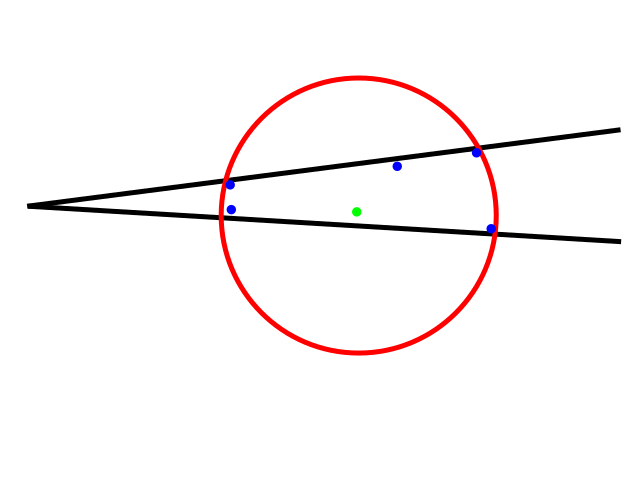
\includegraphics[scale=0.4]{images/bad_lambda.png}
    \caption{Limited sample point choice}
    \label{lspc}
\end{figure}

%As the number of dimensions grows the ratio of volume of the trust region intersect the feasible region to the feasible region can become smaller.

One way to handle this is to introduce a $\xi_{\text{cur}}$ which is allowed to decrease.
(Possibly, until a threshold is reached for maintaining a fixed $\Lambda$.)
If the new point does not improve the geometry of the set significantly, then there is no other point that would do better.
To test this, we introduce a constant $\delta_{\text{improv}}>0$ and require a new point to increase the current pivot by a factor greater than $\delta_{\text{improv}}$.
If the new point does not satisfy this test, we proceed with our current point and possibly decrease $\xi_{\text{cur}}$.
The new modified improvement algorithm is described in \cref{modified_model_improving_algorithm}:

\begin{algorithm}[H]
    \caption{Modified Model Improvement Algorithm}
    \label{modified_model_improving_algorithm}
    \begin{itemize}
        \item[\textbf{Step 0}] \textbf{(Initialization)} \\
            Initialize $i=1$.
            If the current sample set does not have $p$ points, repeat one of the current points. 
            Construct the Vandermonde matrix $V_{i,j} = \phi_j(\frac 1 {\Delta}(y^i - y^0))$.
            Initialize $0 < \ximin < \xi_{\text{desired}}$, $0 <\delta_{\text{improv}} < 1$,
            $  \xi_{\text{cur}} = \xi_{\text{desired}}$.
            
        \item[\textbf{Step 1}] \textbf{(Pivot)} \\
            Swap row $i$ with row $i_{\max} = \arg \max_{j|j\ge i} V_{j,i} $
        
        \item[\textbf{Step 2}] \textbf{(Check threshold)} \begin{itemize}
                \item[] If $|V_{i,i}| \ge \xi_{\text{cur}} $ then go to Step 3
                \item[] $ \hat y = \arg\max_{t \in \sampletrk \cap X} |\phi_i(t)|$
                \item[] If $\label{impossibly_poised} |\phi_i(\hat y)| < \ximin$ then \textbf{Stop}: the algorithm failed
                \item[] If $\xi_{\text{cur}} - |\phi_i(\hat y)| > \delta_{\text{improv}} \xi_{\text{cur}}$ then replace $V_{i,j}$ with $\phi_j(\hat y)$ and $\xi_{\text{cur}} \gets |\phi_i(\hat y)|$
            \end{itemize}
        
        \item[\textbf{Step 3}] \textbf{(LU)} \begin{itemize}
                \item[] Set $V_i \gets \frac{1}{V_{i,i}} V_i$
                \item[] Set $V_{,j} \gets V_{, j} - V_{i,j} V_{\bullet, i} \forall j=i \ldots p$
            \end{itemize}
            $i \gets i+1$
            Go to step 1 unless $i > p$
    \end{itemize}
\end{algorithm}

The \emph{ConstructTrustRegion} subroutine for this approach follows the prototype with $\sampletrk = \searchtrk = \feasiblek \cap \outertrk $.
As is usual, we may also wish to remove points larger than a certain radius from the current model center.
% If a lower bound $\kappa_{\phi}$ on the maximum value of each polynomial is known ahead of time, then the check on \cref{impossibly_poised} is not needed.
% That is, for a given set of linear constraints and largest trust region radius, it may be possible to calculate $\xi_{\text{min}} \le \kappa_{\phi} \le \max_{V}\max_{j}\max_{i}\|\phi_i(y^j)\|$.

%Another interesting approach we have not investigated is to decrease the size of the sample set when a new point cannot be computed.

%The analysis for this approach may be more difficult.




\subsection{Ellipsoidal Trust Region Approach}

If we adopt the ellipsoidal trust region approach to maintain a feasible inner trust region with a ``nice" shape we ensure of a stronger version of \cref{accuracy}.
Namely, we know from \cref{ellipsoidal_lambda} that 
\[
    \|\modelk(x) - \nabla f(x) \| \le \kappa_g \Delta_{k} \quad \forall x \in \innertrk.
\]
If we also choose our trial point with \cref{search_a_little}, we have no guarantee of satisfying the efficiency condition \cref{efficiency} because $\Delta_k$ is the outer trust region radius.
However, the model will likely be more accurate over this region.

%If bounds can be shown relating the model error of the inner trust region to the outer trust region, then we will satisfy \cref{accuracy}.
%In this case, classical methods ensure that $\|\nabla f(x^{(k)}) - \nabla m_f(x^{(k)})\| < \Delta_{inner} \le \Delta_k$.

\subsubsection{Circular Trust Region}
The simplest approach to maintaining a feasible trust region is to set the inner trust region radius sufficiently small.
Within the \emph{ConstructTrustRegion} subroutine, this method sets the trust region radius to the distance to the closest constraint:
$\outertrk = B_2(\iteratek, \min\{\Delta_k, \min_{i}\frac{|A_i\iteratek - b_i|}{\|A_i\|} \})$.
In practice, this does not work well as the radius can become too small to allow adequate progress.

Two general strategies were considered for addressing this issue as illustrated in \cref{options_basis}.
One option is to shift the center of the inner trust region as long as it remains within the outer trust region.
The second option is to elongate the trust region along the nearest constraint as discussed in the next section.
Of course, both of these can be done at the same time.


\begin{figure}[h]
    \centering
    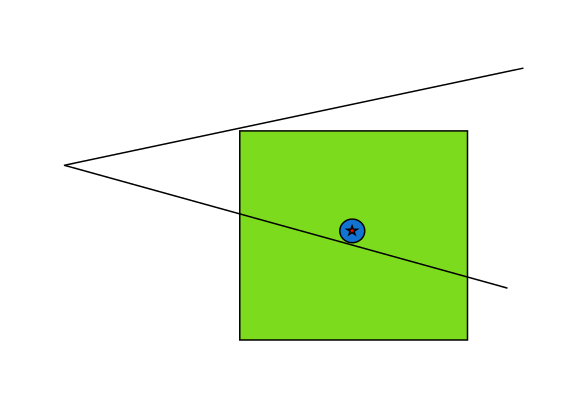
\includegraphics[width=200px]{images/small_circle.png}
    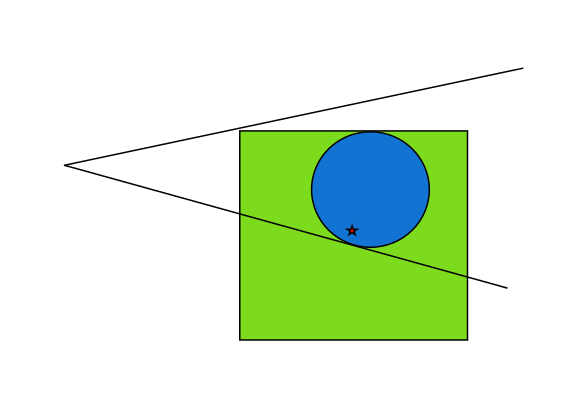
\includegraphics[width=200px]{images/shifted_center.png}
    \caption{When the current iterate is too close to a constraint, the circular trust region becomes too small. Shifting the trust region center helps remedy this. The star is the current iterate, the green is the outer trust region, and blue the inner.}
    \label{options_basis}
\end{figure}

\subsubsection{Ellipsoids}

In order to address this issue we considered using ellipsoidal trust regions.
Whereas the circle does not allow improvement when the current iterate lies along a constraint, an ellipsoid elongates along this constraint.
In figure \cref{ellipse_adv}, we have this type of iterate, but by using an ellipsoid we are still able to search towards the vertex of the feasible region.
\begin{figure}[h]
    \centering
    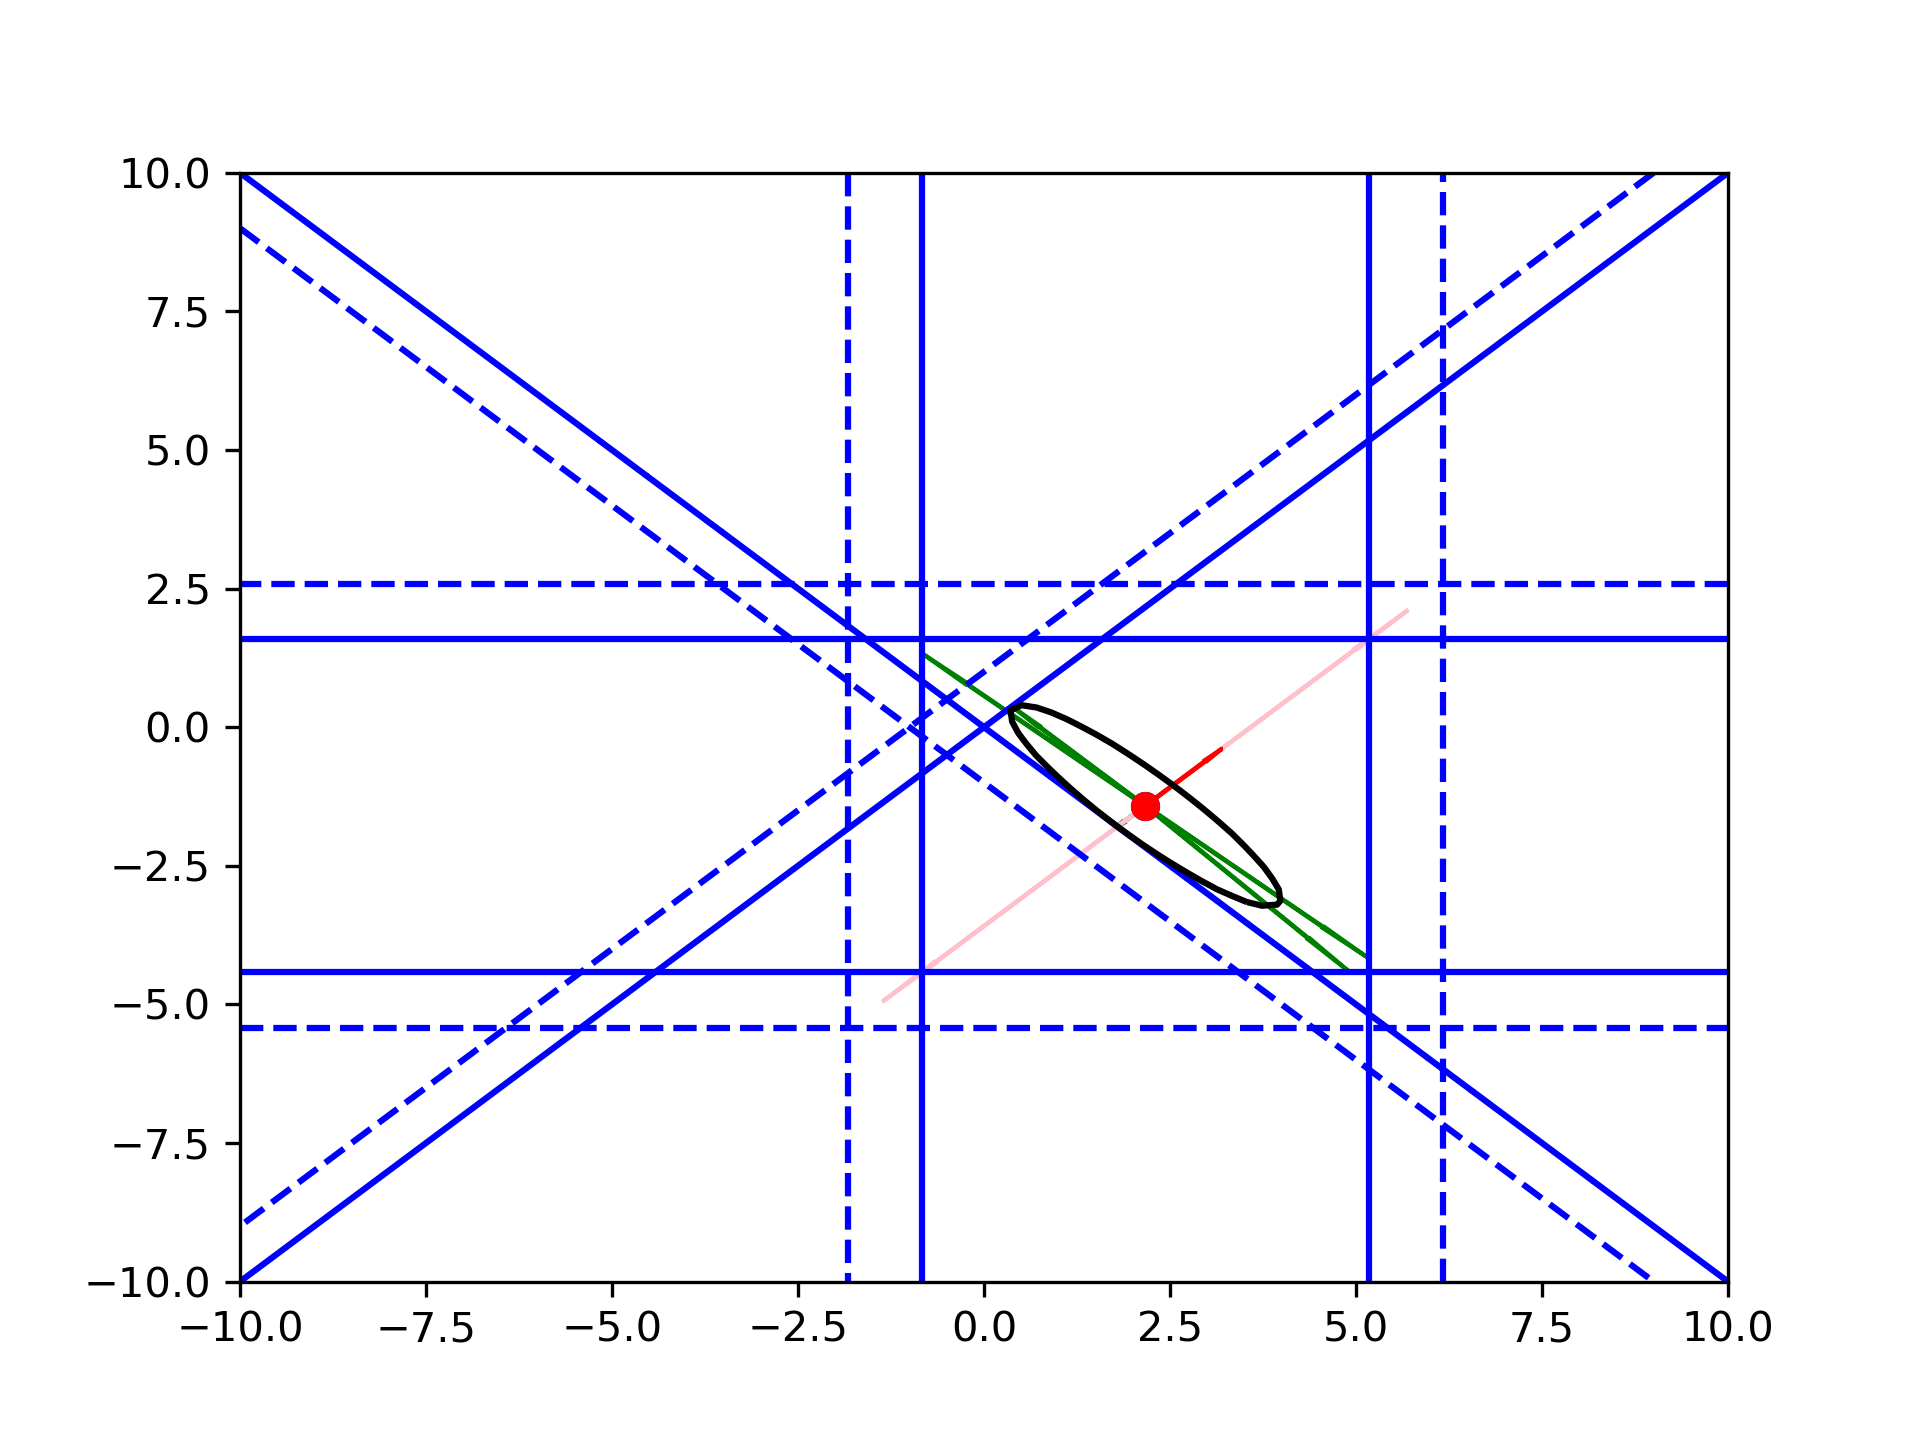
\includegraphics[scale=0.4]{images/advantage_of_ellipse_2.png}
    \caption{A nicer trust region}
    \label{ellipse_adv}
\end{figure}


More specifically, at iteration $k$, we choose a scaling factor $\pi^k$ and solve for an ellipsoid center $\mu^k$ and positive definite matrix $\qk$ to define an ellipsoid
$ \ellipsek = \{x \in \mathbb R^n \| \pi^k - \frac 1 2 (x - \mu^{k})^T\qk(x - \mu^{k}) \ge 0 \}$.
% We then map this back to the origin with the affine transformation $T : \mathbb R^n \to R$, $T(x) = \frac {\sqrt{2}}{\pi^k} L^k(x-\mu^k)$ where $L = cholesky(Q)$.
% This allows us to construct a $\Lambda$-poised set within narrow trust regions.
Of course, the simplest approach is to not change the center of the ellipsoid, but instead let $\mu^k = x^k$.


\subsubsection{Finding the Maximal $ \ellipsek $ Given $\mu^k$}

\label{ellipse_optimization}

Here, we first solve the problem of finding the maximum-volume ellipsoid given the center.
Later we perform a search over different centers of the ellipsoid.
%Because of this, we will first show how to find an ellipsoid with maximum volume given a fixed center.
We adopt a method similar to that described in \cite{Khachiyan1993}.
For now, we also let $\pi^k = 1$.

Given a polyhedron $P$ defined by an $m \times n$ matrix $A$,
\[
P = \{ x \; | \;  Ax \le b \},
\]
we wish to find the maximum-volume ellipsoid $E \subset P$ centered at a point $\mu^{k}$ within this polyhedron.

Let $\bar{b} = b - A\mu^{k}$ and $d = x - \mu^{k}$ so that the polyhedron becomes
\[
P = \{ \mu^k + d \; | \;  Ad \le \bar{b} \}
\]
The ellipsoid can then be centered at zero, and defined by a symmetric positive definite matrix $Q \succ 0$:
\[
E = \{ d \; | \; \frac 1 2 d^T Q d \le 1 \}.
\]
Our goal is to determine $Q$ to maximize the volume of $E$ such that $\mu^{k} + E \subset P$.
Define the auxiliary function 
\[
f(d) = \frac 1 2 d^T Q d
\]
so that 
\[
E = \{ d \; | \; f(d) \le 1 \}.
\]

Because $Q$ is positive definite, $f$ has a unique minimum on each hyper-plane $A_i d = b_i$.
Let this minimum be $d^{(i)} = \argmin_{d\| A_id =\bar{b}_i} f(d)$ for $i=1,\ldots,m$.
By the first order optimality conditions, there exists a $\lambda \in \mathbb R^m$ such that
\[
\nabla f(d^{(i)}) = Q d^{(i)} = \lambda_i A_i \quad \forall 1\le i\le m
\]
\[
\Longrightarrow d^{(i)} = \lambda_i Q^{-1}A_i \quad \forall 1\le i\le m
\]
We also know that 
\[
A_i^T d^{(i)} = \bar{b_i}
\]
\[
A_i^T \lambda_i Q^{-1}A_i = \bar{b_i}
\]
\[
\lambda_i = \frac {\bar{b_i}}{A_i^T  Q^{-1}A_i}
\]
so that 
\[
d^{(i)} = \lambda_i Q^{-1}A_i = \frac {\bar{b_i}}{A_i^T  Q^{-1}A_i}  Q^{-1}A_i \quad \forall 1\le i\le m.
\]

Because $E \subset P$, we also know that $f(d^{(i)}) \ge 1$ for each $i$. Thus,
\[
\frac 1 2 (d^{(i)})^{T} Q d^{(i)} \ge 1
\]
\[
\Longrightarrow \frac 1 2 \bigg(\frac {\bar{b}_i}{A_i^T  Q^{-1}A_i}  Q^{-1}A_i\bigg)^{T} Q \frac {\bar{b}_i}{A_i^T  Q^{-1}A_i}  Q^{-1}A_i \ge 1
\]
\[
\Longrightarrow \frac 1 2 \frac {1}{A_i^T  Q^{-1}A_i}  \bar{b_i} A_i^T Q^{-1} Q \frac {\bar{b_i}}{A_i^T  Q^{-1}A_i}  Q^{-1}A_i \ge 1
\]
\[
\Longrightarrow \frac 1 2 \frac {1}{A_i^T  Q^{-1}A_i}  \frac {\bar{b_i}^2}{A_i^T  Q^{-1}A_i}  A_i^T Q^{-1}A_i \ge 1
\]
\[
\Longrightarrow \frac 1 2  \frac {\bar{b_i}^2}{A_i^T  Q^{-1}A_i} \ge 1
\]
\[
\Longrightarrow \frac 1 2 \bar{b_i}^2\ge A_i^T  Q^{-1}A_i
\]
\[
\Longrightarrow A_i^T  Q^{-1}A_i \le \frac 1 2 \bar{b_i}^2
\]

Because the volume of the ellipsoid is proportional to the determinant of $Q^{-1}$, the maximal ellipsoid is defined by

\[
\qk = V(\mu^k) = \sup_{Q \succeq 0} \det(Q^{-1})
\]
\[
s.t. \quad A_i^T Q^{-1} A_i \le \frac 1 2 \bar{b_i}^2
\]


%This problem includes a maximization of a determinant.
%In order to ensure that the trust region goes to zero, we must also ensure that the maximum eigenvalue of the matrix is bounded.
%Thus, for some bound $M^k$ we define $Q^k$ as
%  & eig(Q)_i \le M^k & \forall i \in \mathcal I \cup \mathcal E \\

After shifting the center to $\mu^{k}$, this problem takes the form:

\begin{center}
\begin{align}
\label{ellipse_1}
\qk = V(\mu^k) = \sup_{Q \succ 0} & \det(Q^{-1}) & \\
  & {A^k}_i^T Q^{-1} {A^k}_i \ge \frac 1 2 (b^k - A^k\mu^{k})^T(b^k - A^k \mu^{k}) & \nonumber
\end{align}
\end{center}


%  & \pi^k - \frac 1 2 (x^k - \mu^{k})^TQ^{k}(x^k - \mu^{k}) \ge 0

%if we wish to include the original point explicitly.
%This gives rise to the trust region sub problem of
%
%$$\innertrk = \{x \in \mathbb | 1 - \frac 1 {2\pi^k} (x - \mu^{k})^T Q (x - \mu^{k}) \ge 0\} $$
%$$ \pi^k = \max \{1, \frac 1 {2} (\iteratek - \mu^{k})^T Q^k (\iteratek - \mu^{k})^T \}$$

\subsubsection{Poisedness over Ellipsoidal Trust Regions}
\label{ellipsoidal_lambda}

% TODO: Find a better reference
It is possible to show $\Lambda$-poisedness for an ellipsoidal region with a change of variables to the ball centered around the origin.
We wish to construct a model for $f(x)$ in the ellipsoidal region
$\ellipsek = \{x \in \mathbb R^n | (x - c)^T\qk(x - c) \le 1\}$ for some symmetric, positive definite
$\qk \in \mathbb R^{n\times n}$ and some center $c \in \mathbb R^n$.
We can give $\qk$ its eigen-decomposition $\qk = L D^2 L^T$, where $L^TL = I$ and $D$ is a diagonal matrix with nonnegative entries.
If we let $\delta = \max_{x\in \ellipsek}\|x-c\|$, then the transformation $T(x) = \delta DL^T(x - c)$ maps $ \ellipsek $ to the $\delta$ ball $\{u = T(x) \in \mathbb R^n \; | \; \|u\| \le \delta\}$.
Conversely, $ T^{-1}(u) = \frac 1 {\delta} LD^{-1}u + c$ maps the $\delta$ ball to the ellipsoidal region $ \ellipsek $.

% \cref{fully_quadratic}

\begin{theorem}
Let $T$ and $\delta$ be as defined above, and let $\hat m_f(u)$ be a model of the shifted objective $\hat f(u) = f(T^{-1}(u))$ in the $\delta$ ball such that
there exist constants $\kappa_{ef}, \kappa_{eg}, \kappa_{eh} > 0$ such that for all $\{u \in R^n | \;\|u\| \le \delta \}$, we have
% for all $u \in B(0 ; \delta)$ we have the following error bounds:
\begin{align*}
|\hat m_f(u) - \hat f(u)| \le \kappa_{ef} \delta^3\\
\|\nabla \hat m_f(u) - \nabla \hat f(u)\| \le \kappa_{eg}\delta^2\\
\|\nabla^2 \hat m_f(u) - \nabla^2 \hat f(u)\| \le \kappa_{eh}\delta.
\end{align*}

Then, with
\begin{align*}
\kappa_{ef}' = \kappa_{ef} \\
\kappa_{eg}' = \kappa_{eg}\sqrt{\kappa(\qk)} \\
\kappa_{eh}' = \kappa_{eh}\kappa(\qk),
\end{align*}
we have that for all $x \in \ellipsek$,
the model function $m_f(x) = \hat m_f(T(x))$ will satisfy
\begin{align*}
| m(x) - f(x)| \le \kappa_{ef}'\delta^3 \\
\|\nabla  m(x) - \nabla  f(x)\| \le \kappa_{eg}'\delta^2 \\
\|\nabla^2 m(x) - \nabla^2 f(x)\| \le \kappa_{eh}'\delta.
\end{align*}
\end{theorem}

\begin{proof}

% Notice  that for all $x\in \ellipsek$ we have 
% \begin{align*}
% \|x-c\| \le \delta \\
% \|T(x-c)\| \le \delta \\
% \end{align*}
% so that $\frac{\|T(x-c)\|}{\|x-c\|} \le 

We know that $\delta = \frac 1 {\sqrt{\lambda_{\text{min}}(\qk)}} = \frac 1 {\min_{i} D_{i, i}}$.
This means,
\begin{align*}
\kappa(\qk) = \kappa(D^2) = \frac{\max_{i}D_{i,i}^2}{\min_{i}D_{i,i}^2} = \delta^2 \max_{i}D_{i,i}^2 = \delta^2 \|D\|^2 \\
\|D\| = \frac 1 {\delta} \sqrt{\kappa(\qk)} \le \frac{\kappa_{\lambda}}{\delta}.
\end{align*}

Also, $\delta \le \dk$ as the ellipse is constructed within the outer trust region.
\color{red}
% For all $x \in  \ellipsek$, we have that
% \begin{align*}
% \delta^2 \lambda_{\text{min}}(Q) \le \lambda_{\text{min}}(Q) (x-c)^T(x-c) \le (x-c)^TQ(x-c) \le 1 \\
% \lambda_{\text{max}} x^T x\le 1 \\
% \|x\|^2 \le \frac 1 {\lambda_{\text{max}}} \\
% \|x\| \le \frac 1 {\sqrt{\lambda_{\text{max}}}} \\
% \end{align*}


% Notice that because $\ellipsek \subset T(\ellipsek)$ and $\|T(x-c)\| = \|x-c\|$ along the major axis, we must have $\lambda_{\text{min}}(T) = 1$.
% This means that $\delta min_{i} D_{i,i} = 1 \Longrightarrow \delta = \frac{1}{\min_{i}D_{i,i}}$.
% Because the major axis of the ellipse is preserved, we also
% smallest eigenvalue of $T$ is $1$.
% \begin{align*}
% \kappa(Q) = \kappa(D^2) = \frac{\max_{i}D_{i,i}^2}{\min_{i}D_{i,i}^2} \ge \delta^2 \max_{i}D_{i,i}^2 = \delta^2\|D\|^2
% \end{align*}

\color{black}

Then, we have for all $\{u = T(x) \; | \; \|u\| \le \delta \} \Leftrightarrow x \in \ellipsek$

%\Leftrightarrow \{x = T^{-1}(u) \; | \; \|T^{-1}(u)\| \le 1 \} 

% \begin{align*}
% \delta^2\kappa(Q) = \|D\|
% \end{align*}
% smallest eigenvalue of t is one
% 

\begin{align*}
 | m_f(x) - f(x)| = |\hat m(u) - \hat f(u)| \le \kappa_{ef}'\dk^3.
\end{align*}

Similarily, for the gradient we find:

\begin{align*}
\| \nabla m_f(x) - \nabla f(x)\| = \delta\left\|DL^T\left(\nabla\hat m_f(u) - \nabla \hat f(u)\right)\right\| \le \delta \|DL^T\|\|\nabla \hat m_f(u) - \nabla \hat f(u)\| \le \sqrt{\kappa(\qk)}\kappa_{eg} \delta^2 \\
\end{align*}

% \begin{align*}
% \|\nabla \hat m_f(u) - \nabla \hat f(u)\| \le \Lambda \kappa_{eg} \delta^2\\
% \|\nabla ( m_f(T^{-1}(u))) - \nabla ( f(T^{-1}(u)))\| \le \Lambda \kappa_{eg} \delta^2\\
% \|\nabla \left( m_f(\frac 1 {\delta} D^{-T}L^Tu + c)\right) - \nabla \left( f(\frac 1 {\delta} D^{-T}L^Tu + c)\right)\| \le \Lambda \kappa_{eg} \delta^2\\
% \|\frac 1 {\delta} LD^{-1} \nabla  m_f(\frac 1 {\delta} D^{-T}L^Tu + c) - \frac 1 {\delta} LD^{-1} \nabla  f(\frac 1 {\delta} D^{-T}L^Tu + c)\| \le \Lambda \kappa_{eg} \delta^2\\
% \|LD^{-1} \left(\nabla  m_f(x) - \nabla  f(x)\right)\| \le \Lambda \kappa_{eg} \delta^3\\
% \|DL^T\|\|LD^{-1} \left(\nabla  m_f(x) - \nabla  f(x)\right)\| \le \Lambda \kappa_{eg} \delta^3 \left(\frac {\kappa_{\lambda}} {\delta}\right) \\
% \|\nabla  m(x) - \nabla  f(x)\| \le \Lambda \kappa_{eg}' \delta^2 \le \Lambda \kappa_{eg}' \dk^2. \\
% \end{align*}
Finally, we show that for the Hessian:

\begin{align*}
\| \nabla^2 m_f(x) - \nabla^2 f(x)\| = \delta^2\left\|DL^T\left(\nabla\hat m_f(u) - \nabla \hat f(u)\right)LD^T\right\| \le \delta^2 \|D\|^2\|\nabla \hat m_f(u) - \nabla \hat f(u)\| \le \kappa(\qk)\kappa_{eh} \delta \\
\end{align*}

% \begin{align*}
% \|\nabla^2 \hat m_f(u) - \nabla^2 \hat f(u)\| \le \Lambda \kappa_{eh} \delta\\
% \|\nabla^2 \left(m_f(\frac 1 {\delta} D^{-T}L^Tu + c)\right) - \nabla^2 \left(f(\frac 1 {\delta} D^{-T}L^Tu + c)\right)\| \le \Lambda \kappa_{eh} \delta\\
% \frac 1 {\delta^2} \|LD^{-1} \nabla^2 m_f(\frac 1 {\delta} D^{-T}L^Tu + c) D^{-T}L^T - LD^{-1} \nabla^2 f(\frac 1 {\delta} D^{-T}L^Tu + c) D^{-T}L^T\| \le \Lambda \kappa_{eh} \delta\\
% \|LD^{-1} \left(\nabla^2 m_f(x) - \nabla^2 f(x) \right) D^{-T}L^T\| \le \Lambda \kappa_{eh} \delta^3 \\
% \|DL^T\|\|LD^{-1} \left(\nabla^2 m_f(x) - \nabla^2 f(x) \right) D^{-T}L^T\|\|LD\| \le \Lambda \kappa_{eh}\delta^3\left(\frac {1}{\delta^2}\kappa(\qk)\right)  \\
% \|\nabla^2 m_f(x) - \nabla^2 f(x)\| \le \Lambda \kappa_{eh}' \delta \le \Lambda \kappa_{eh}' \dk\\
% \end{align*}




% \begin{align*}
% \min_{i}D_{i,i} = \frac{\dk }{\text{length longest axis of ellipse}} \\
% \frac{1}{\min_{i}D_{i,i}} = \frac{\text{length longest axis of ellipse}}{\dk } \le 1\\
% \frac{1}{\min_{i}D_{i,i}^2} = \bigg(\frac{\text{length longest axis of ellipse}}{\dk }\bigg)^2 \le 1\\
% \kappa(Q) = \max_i D_{i,i}^2 \bigg(\frac{\text{length longest axis of ellipse}}{\dk }\bigg)^2 \le \max_i D_{i,i}^2\\
% \kappa(Q) = \frac{\max_{i}D_{i,i}^2}{\min_{i}D_{i,i}^2} = \|D\|\delta \le \kappa_{\lambda} \\
% \|DL^T\| \le \frac{\kappa_{\lambda}}{\delta}\\
% \end{align*}

\end{proof}

This shows that in order to have strongly quadratic model functions, we need only bound the condition number of $\qk$.
For the purposes of a convergence proof, we need only satisfy the weaker accuracy condition \cref{accuracy}.
Notice that in practice the model functions do not need to be mapped to the $\delta$ ball, because $\Lambda$-poisedness is scale invariant \cite{DUMMY:intro_book}.
The implications of this proof are discussed futher in the convergence discussion \cref{convergence_discussion}.

% After constructing a $\Lambda$-poised set on the unit ball, we can construct a shifted model function
%  that accurately models a shifted objective  over a ball.
% Namely, from , we know that for some constants , we have that for all :
 

% Letting $\delta = \frac 1 {\min_i D_{i,i}^2}$, and forcing the condition number of $Q$ to be less than or equal to a fixed constant $\kappa_{\lambda}$, we see that
%\color{red}
%We notice that the length of the largest axis of the ellipsoid is bounded by $\dk$, so that $\min_{i}D_{i,i}^2 \le \dk$.
%\color{black}

%Given a constant $\kappa_{\lambda} > 0$, we force 
%so that


% right hand sides are one
% little delta is the max|x-c|, x \in  E
% T(x) = little delta DL^T(x - c)
% smallest eigenvalue of t is one
% \kappa(little delta ^2 Q) = \|D\|
% mapping onto little delta



%These new constants $\kappa_{ef}', \kappa_{eg}', \kappa_{eh}'$ depend only on the largest eigenvalue of $Q$.

\subsubsection{Ellipsoid Choices}

There are a number of issues to be solved to define this ellipsoid:
\begin{itemize}
\item How do we ensure that $\iteratek \in \ellipsek $?
\item How do we choose $\ellipsek$ in such a way that it does not limit travel along a decent direction?
\item How do we choose the center of the ellipsoid $\mu^k$?
\end{itemize}

% \item How do we choose $\ellipsek$ to make the  ellipsoid as large as possible while ensuring that $ \ellipsek \subset \outertrk \cap \feasiblek $?

If $\iteratek \not \in \searchtrk $, the ellipse may not even contain a point with any reduction.
Thus, we have implemented a few ways of ensuring the current iterate is within the search trust region.
This can be done by either of the following two options:
\begin{itemize}
\item Adding a constraint to the ellipsoid problem to include the original point.
\item Expand the size of the ellipsoid.
\end{itemize}

%IMAGES GO HERE

\paragraph{Adding a constraint.}
In order to include the original point as a constraint, we add a constraint to the definition of the ellipsoid of the following form:
$$ \pi^k - \frac 1 2 (x^k - \mu^{k})^T\qk(x^k - \mu^{k}) \ge 0. $$
Constraints of this nature make finding the ellipsoid much more expensive.
This is because the optimization problem we construct uses ${\qk}^{-1}$ as decision variables, so that constraints in terms of $\qk$ must model matrix inversion.

\paragraph{Increase the size.}
An alternative is to scale $\qk$ by a constant.
We use the scaling factor $\pi^k$ defined by

$$\pi^{(k)} = \max \{1, \frac 1 {2} (x^{k} - \mu^{k})^T \qk (x^{k} - \mu^{k})^T \}$$

and let the ellipsoid be:
$$\ellipsek = \{x \in \mathbb | 1 - \frac 1 {2\pi^k} (x - \mu^{k})^T \qk (x - \mu^{k}) \ge 0\} $$
However, this means that in general $\ellipsek \not \subset \feasiblek$ so that the trust region subproblem must contain constraints for both the ellipsoid and the feasible region: $\searchtrk = \ellipsek \cap \domain$.

To help mitigate the second issue, we maximize the volume of the ellipsoid.
However, the choice of ellipsoid center can still limit travel along a decent direction.
Choosing the best center is the topic of the next section.

\paragraph{One theoretical concern}

%The are some other concerns to be considered while defining the ellipsoid.
% While choosing $\ellipsek$, 

%We also want consecutive ellipsoid to share volume, in order to avoid evaluating as many points as possible.
%(So far, we have been re-evaluating the set of trial points each iteration.)


Lastly, when $\ellipsek \subset \feasiblek$, we may not be able find a second order solution.
This is becase the ellipsoid can only be tangent to the constraint, and some decent paths may be missed.
In \cref{fbns}, the red line represents a path in the feasible region that is always decreasing.
However, if the trust regions decrease without intersecting this path, the algorithm will not be aware of this descent path.
However, scaling the trust region to the outer green radius may allow the algorithm to ensure global convergence to second order critical points.

\begin{figure}[h]
    \centering
    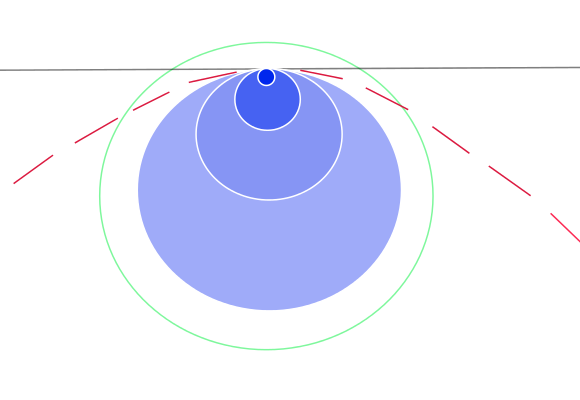
\includegraphics[width=200px]{images/second_order_critical_point.png}
    \caption{Potential issue with a second order critical point.}
    \label{fbns}
\end{figure}



% Finally, we have the problem of computing the ellipsoid once given a suitable definition.


\subsection{Searches for the Center}

We consider several different approaches for determining the trust region center $\mu^k$.
In this case, our \emph{ConstructTrustRegion} subroutine searches over multiple centers of the ellipsoid, however it may not need to construct the model functions for each until it has found a desirable ellipsoid.




%For now, we maximize the volume of $E_k$, .

%For now, we have simply used the heurstic $H(E_k) \to \text{Vol}(E_k)$.
%Given a huristic $H : \innertrk \to \Theta$, where $\Theta$ is a set of comparable elements, the \emph{ConstructTrustRegion} routine follows the following template:

%\begin{algorithm}[H]
%    \caption{Heuristic Search}
%    \label{heuristic_search}
%    \begin{itemize}
%        \item[] \textbf{Initialization} Initialize $T_{\text{best}} = \emptyset$, $\theta_{\text{best}} = H(T_{\text{best}})$
%            
%        \item[] \textbf{For all $\mu \in$ search space do:} \begin{itemize}
%                \item[] $T_{\text{trial}} \gets \arg\max_{E_k \text{centered at} \mu} \text{Vol}(E_k)$
%                \item[] $\theta_{\text{trial}} = H(T_{\text{trial}})$
%                \item[] If $\theta_{\text{trial}} \le \theta_{\text{best}}$ then continue
%                \item[] $T_{\text{best}} = T_{\text{trial}}$
%                \item[] $\theta_{\text{best}} = \theta_{\text{trial}}$
%            \end{itemize}
%    \end{itemize}
%\end{algorithm}


\subsubsection{Search Everything}

One approach is to search all possible centers within $ \feasiblek \cap \outertrk $.
That is, we solve:
$$\mu^k = \sup_{\mu \in \feasiblek \cap \outertrk} V(\mu)$$
where $V(\mu)$ is the volume of the ellipsoid defined in \cref{ellipse_1}.
%The search within the \emph{ConstructTrustRegion} is allowed to go anywhere within $ \feasiblek \cap \outertrk$.
This has the advantage that it captures much of the feasible region.
However, one problem with this search is that it can force the trust region away from the desired direction.
Notice that in \cref{ellipse_runs_away}, although the ellipsoid found has larger volume than before being shifted, this ellipsoid contains points farther from the corner containing the minimizer.

\begin{figure}[h]
    \centering
    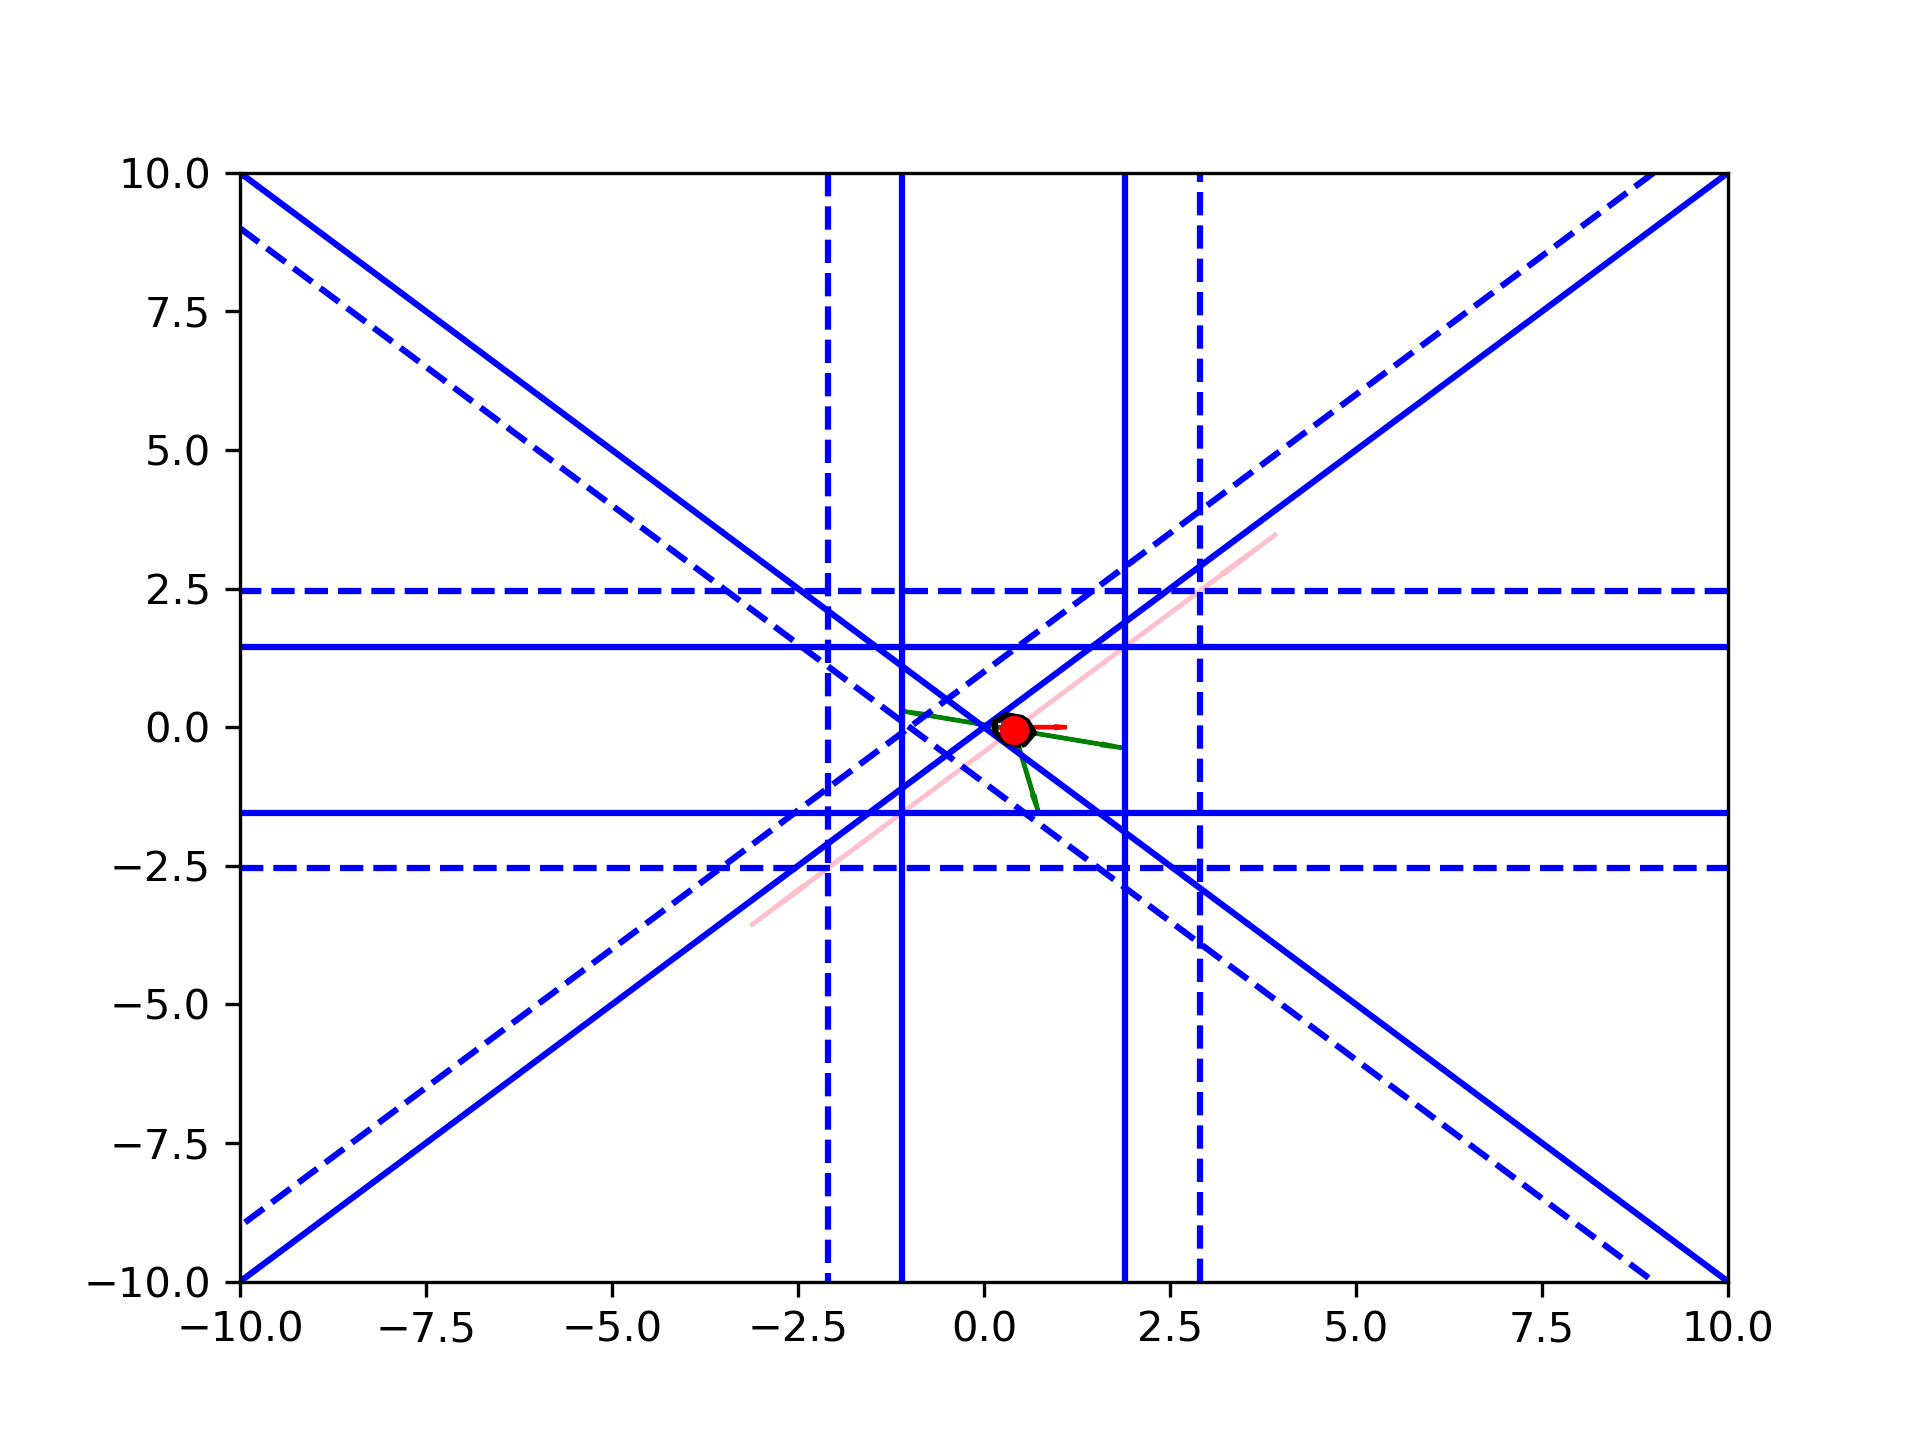
\includegraphics[scale=0.4]{images/everything_runs_1.png}
    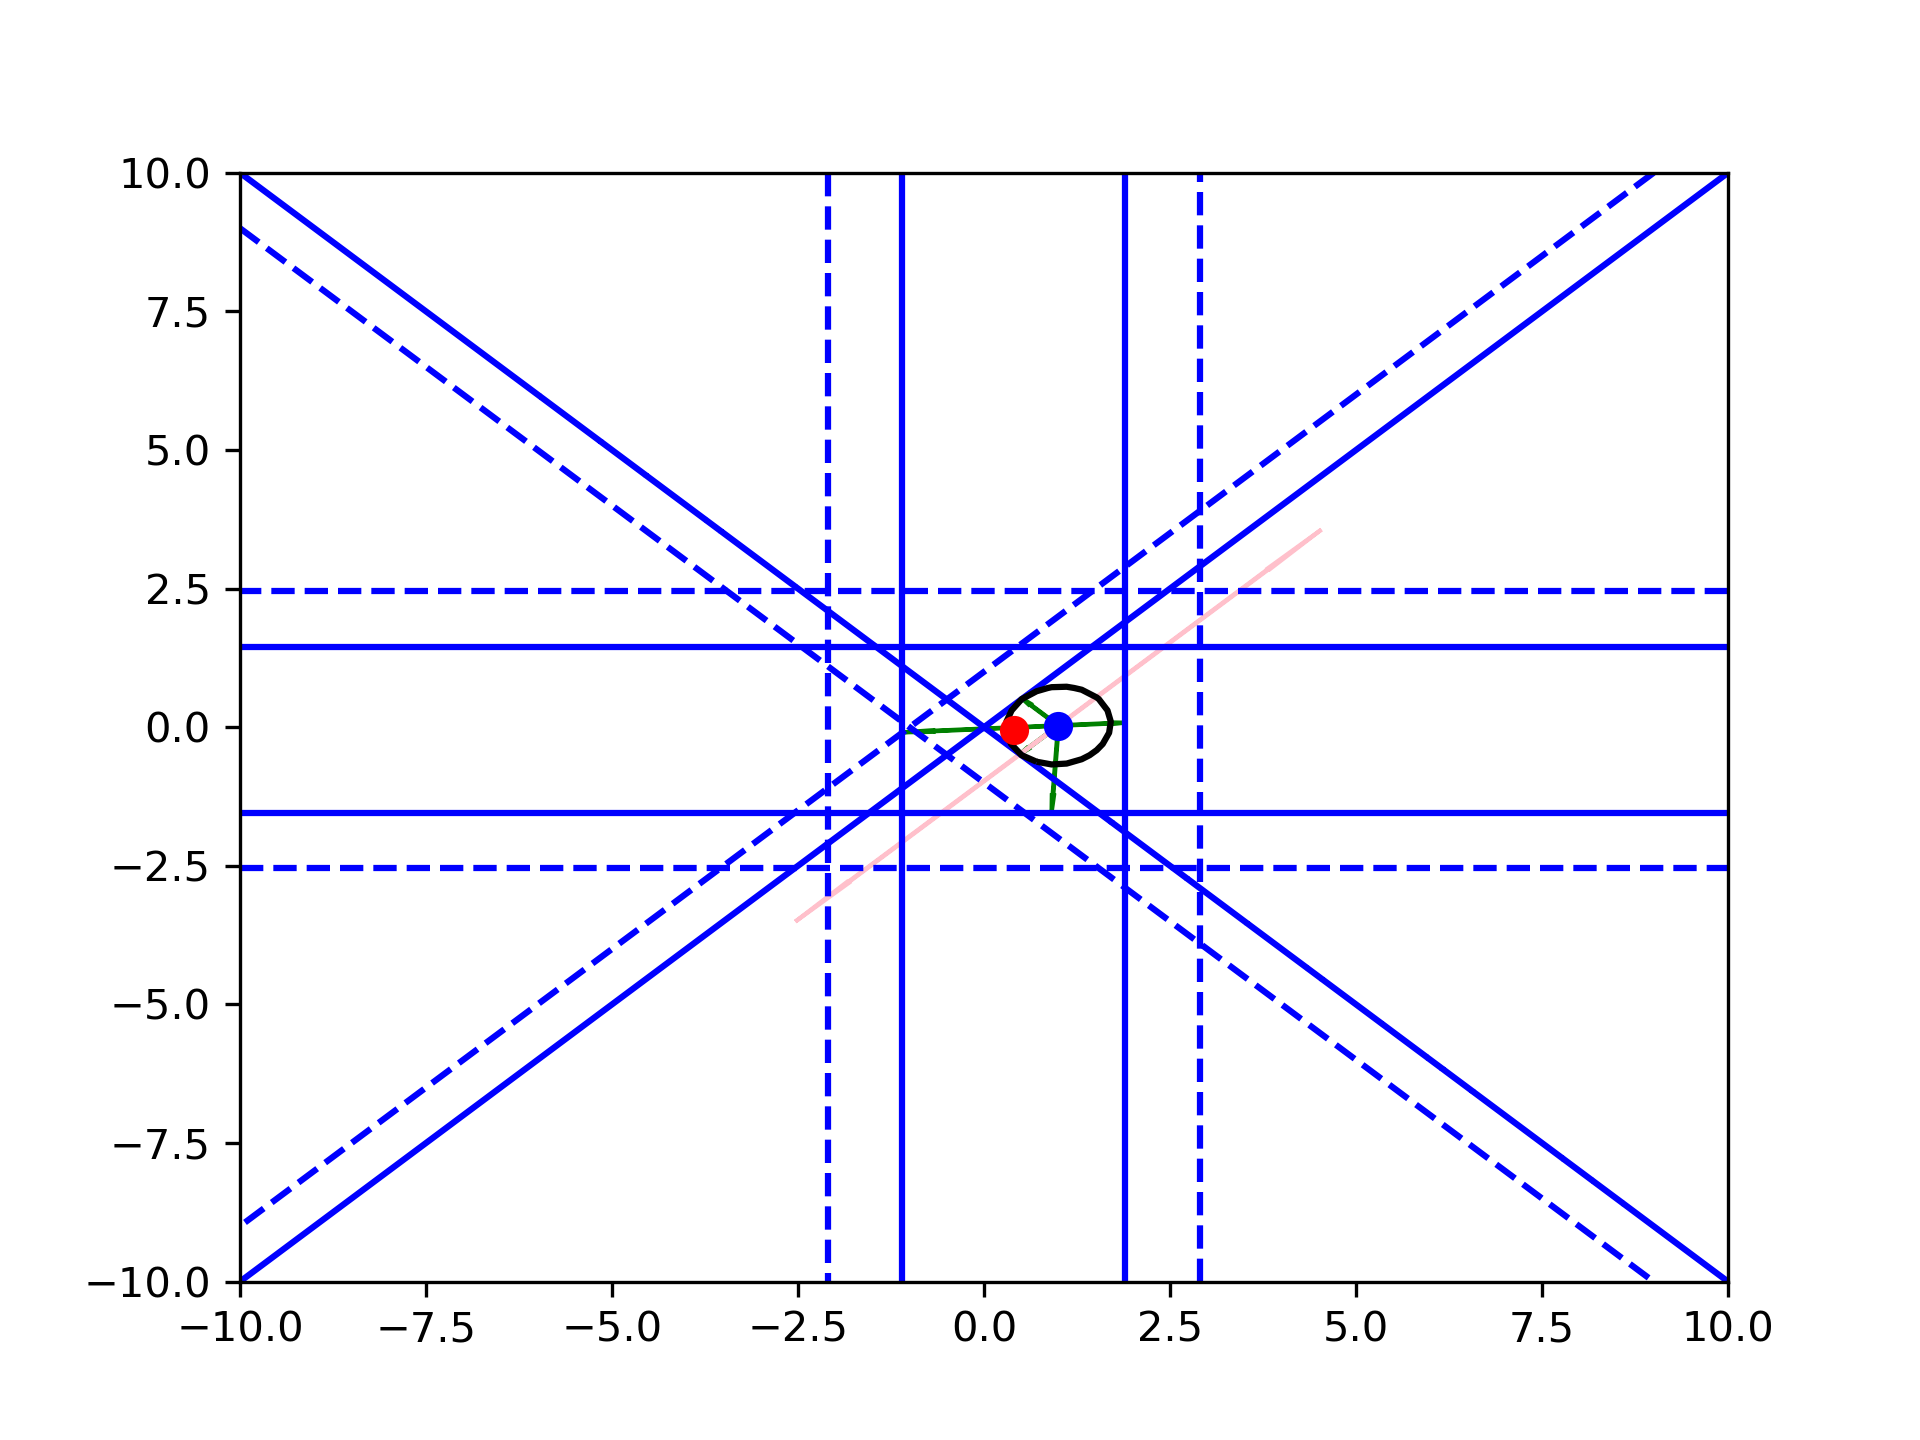
\includegraphics[scale=0.4]{images/everything_runs_2.png}
    \caption{Searching $\feasiblek$}
    \label{ellipse_runs_away}
\end{figure}


One attempt to fix this problem is by limiting the search direction for the center of the ellipsoid.


\subsubsection{Line Searches}
Although $\modelk$'s minimizer over $\outertrk$  can appear anywhere, there are some reasons for expecting it to be at a ``vertex."
If it lies in the interior, there is little need for using constrained approaches once near the solution.

%The ellipsoid with maximum volume, however, tends to lead $ \sampletrk $ away from vertices.
One way of trying to ensure a feasible direction towards a vertex, while still allowing a larger volume ellipsoid, is by limiting the search for the new center to lie on line segments starting at the current iterate $\iteratek$.

For example, our first attempt was to simply search a line directed orthogonally away from the closest constraint.
This has obvious problems as shown in \cref{first_line_search}, as we should avoid letting the new center get closer to another constraint:

\begin{figure}[h]
    \centering
    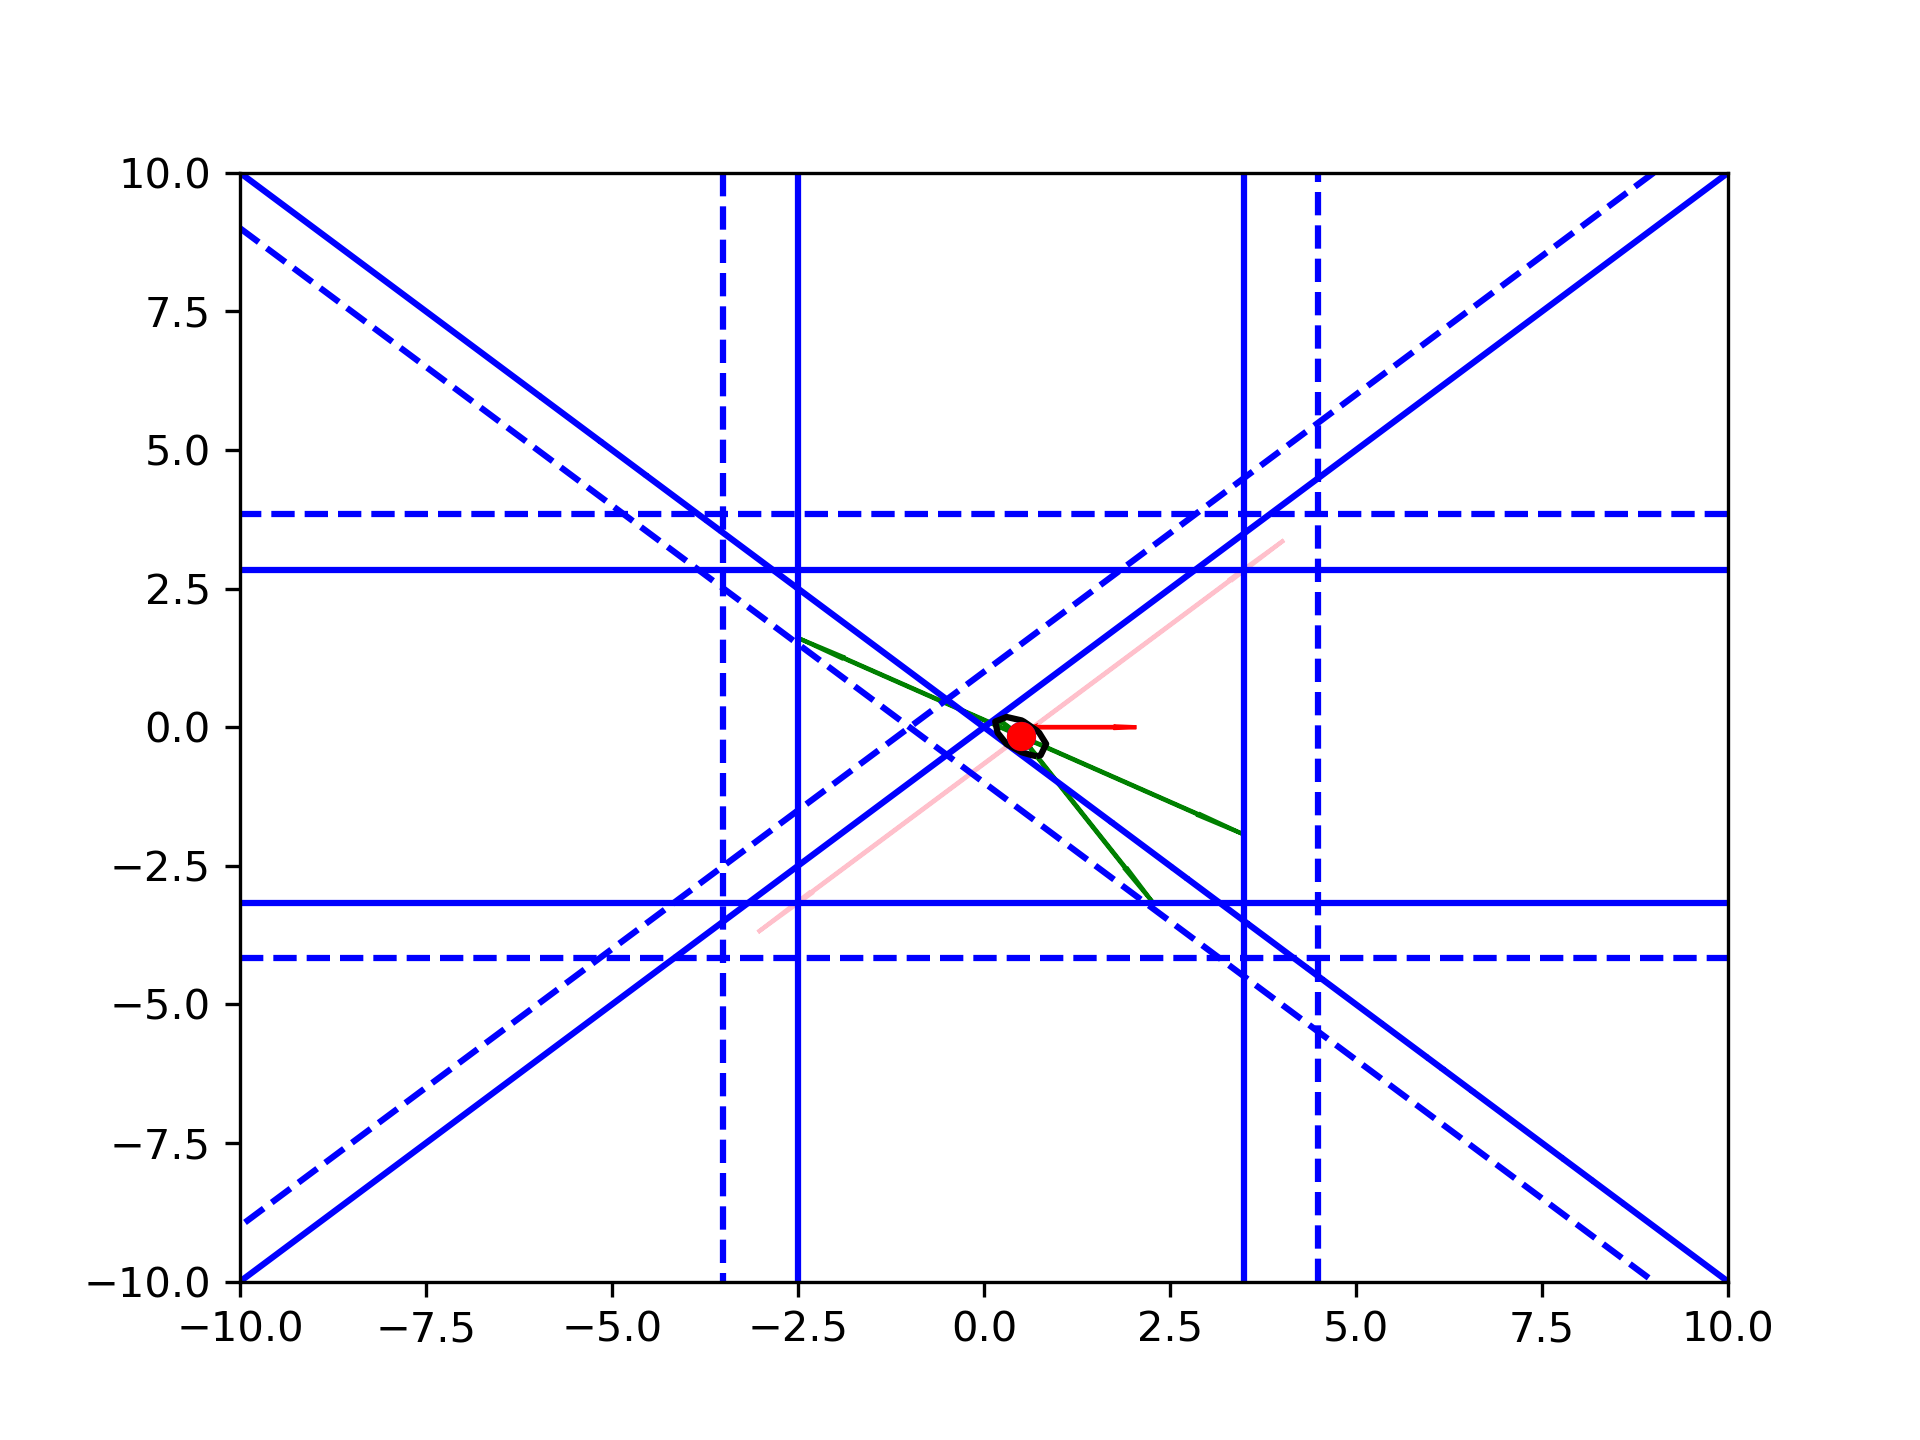
\includegraphics[scale=0.4]{images/line_1.png}
    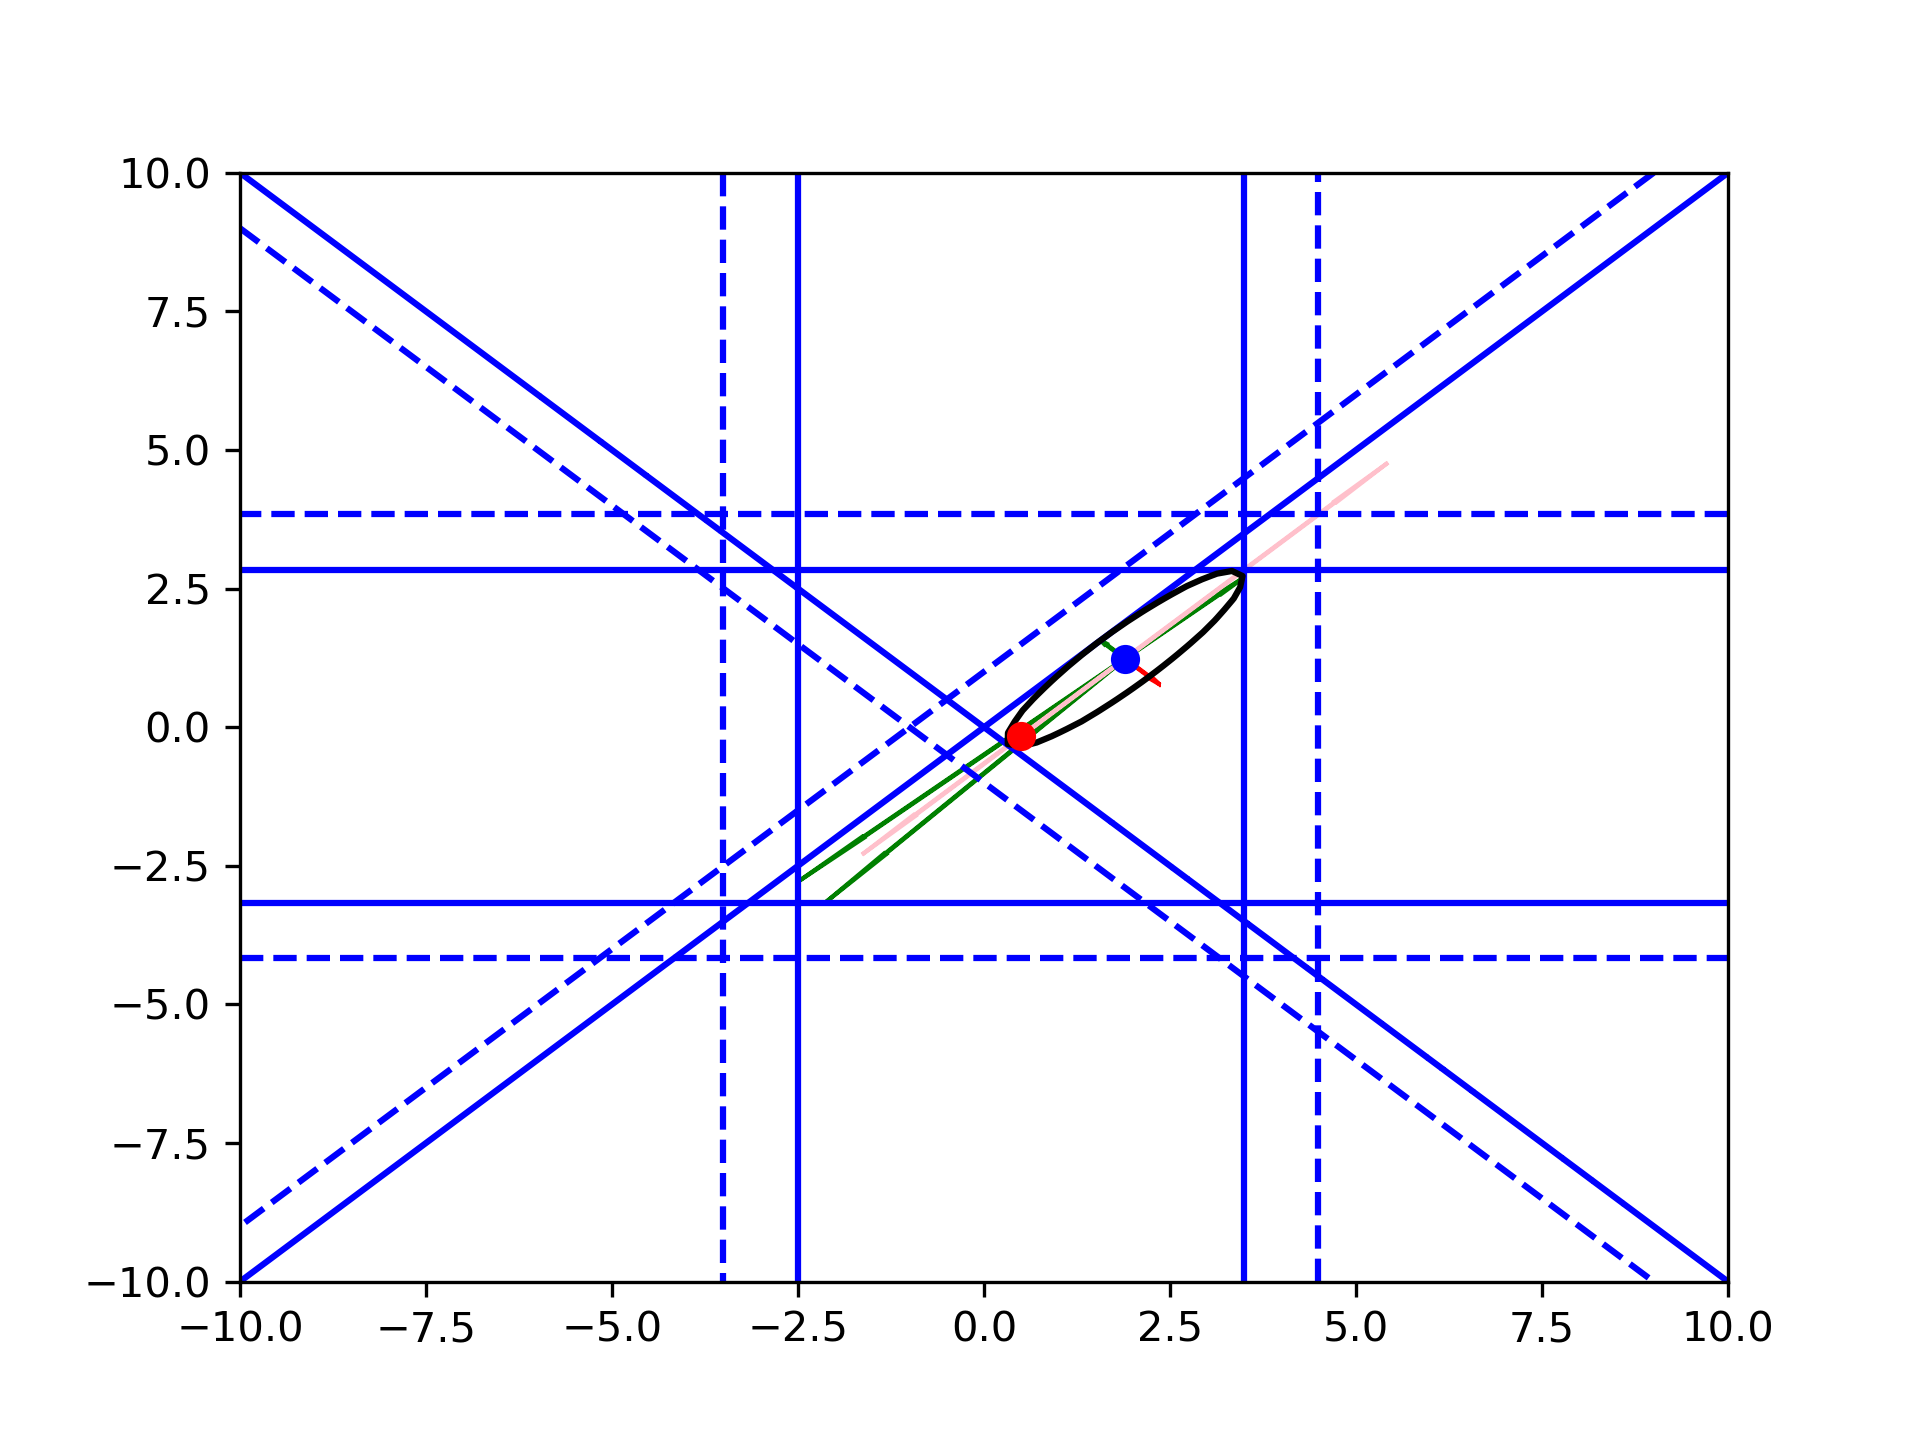
\includegraphics[scale=0.4]{images/line_2.png}
    \caption{Line searches}
    \label{first_line_search}
\end{figure}


For a given distance $d$, let the indices $i$ for which $\frac {|A_i x - b|}{\|A_i\|} \le d$


To fix this, we break the search space within the \emph{ConstrucTtrustRegion} subroutine into segments based on the nearest constraints.
The algorithm works by choosing a set of up to $n_{\text{points}}$ points $s_1, s_2, \ldots, s_{n_{\text{points}}}$ that are each equidistant to a subset of the constraint's faces.
The center search then considers points along the line segments between these points.
% Namely, it starts at the current iterate and travels along a ray away from all the closest constraints until it reaches a point equidistant to yet another constraint.

More precisely, the first point is chosen to be the current iterate: $s_1 = \iteratek$.
The algorithm then repeats the following process for $i$ from $1$ to $n_{\text{points}}$.
First, compute the set of nearest constraints, where the distance from a point $x$ to a constraint $A_i$ is given by $d(A_i, x) = \frac {|A_i x - b|}{\|A_i\|}$.
While finding the next point $s_{i+1}$, let  $A_E$ be a normalized array of the equidistant faces $\{\frac{A_i}{\|A_i\|} | d(A_i, s_i) = \min_j d(A_j, s_i), i = 1, 2, \ldots, m\}$ and $b_E$ be the rows' corresponding values of $b$.
All other faces are called the remaining faces, and construct the matrix $A_R$ and vector $b_R$.
It then finds a search direction $p  = r{A_E}^T$ as a linear combination of the normal vectors to the equidistant faces.
%When the constraint violation of $s_i$ is non-zero, this search ray can be found by finding the point that doubles the current slack ${A_E}s_i-{b_E}$.
%This is given by $r{A_E}^T$ where $r$ solves the linear system ${A_E}(s_i + r{A_E}^T) - b_E = 2 ({A_E}n_i - b_E)$.
%If the current violation is zero, then the right hand side can be set to a vector of all ones to ensure that all slacks violations are the same: $A_E(s_i + r{A_E}^T) - b_E = 1$.
This search ray can be found by setting the slack to each equidistant face to a vector of all ones: $A_E(s_i + r{A_E}^T) - b_E = 1$.
We can travel along this ray until we reach a point that is the same distance to a remaining face.
Specifically, we can travel by 
\begin{align}
t = \argmin_j {\frac{d({A_E}_0, s_i) - d({A_R}_j, s_i)}{ {A_R}_j - d({A_E}_0) p} | ({A_R}_j - d({A_E}_0) p > 0 }. 
\end{align}

We can then set $s_{i+1} = s_{i} + t p$.

Of course, $n_{\text{points}}$ must be less than or equal to $n + 1$ in order for this to be defined.
Also, the algorithm must stop early if $A_E$ contains parallel faces.

% if we let $\nabla \modelconstrainti(\iteratek) = A_i$ be the $i$th row of $A$, then we define the distance from a search point $s$ so the $i$th constraint to be


This means that we can define a class of searches that each limit the number of line segments to search $n_{\text{points}}$.

In figure \cref{line_can_run}, the red line shows the line segments equidistant their closest constraints.
Notice that with two line segments, the algorithm can already choose new centers further from the vertex.

% TODO: REPLACE PICTURES
\begin{figure}[h]
    \centering
    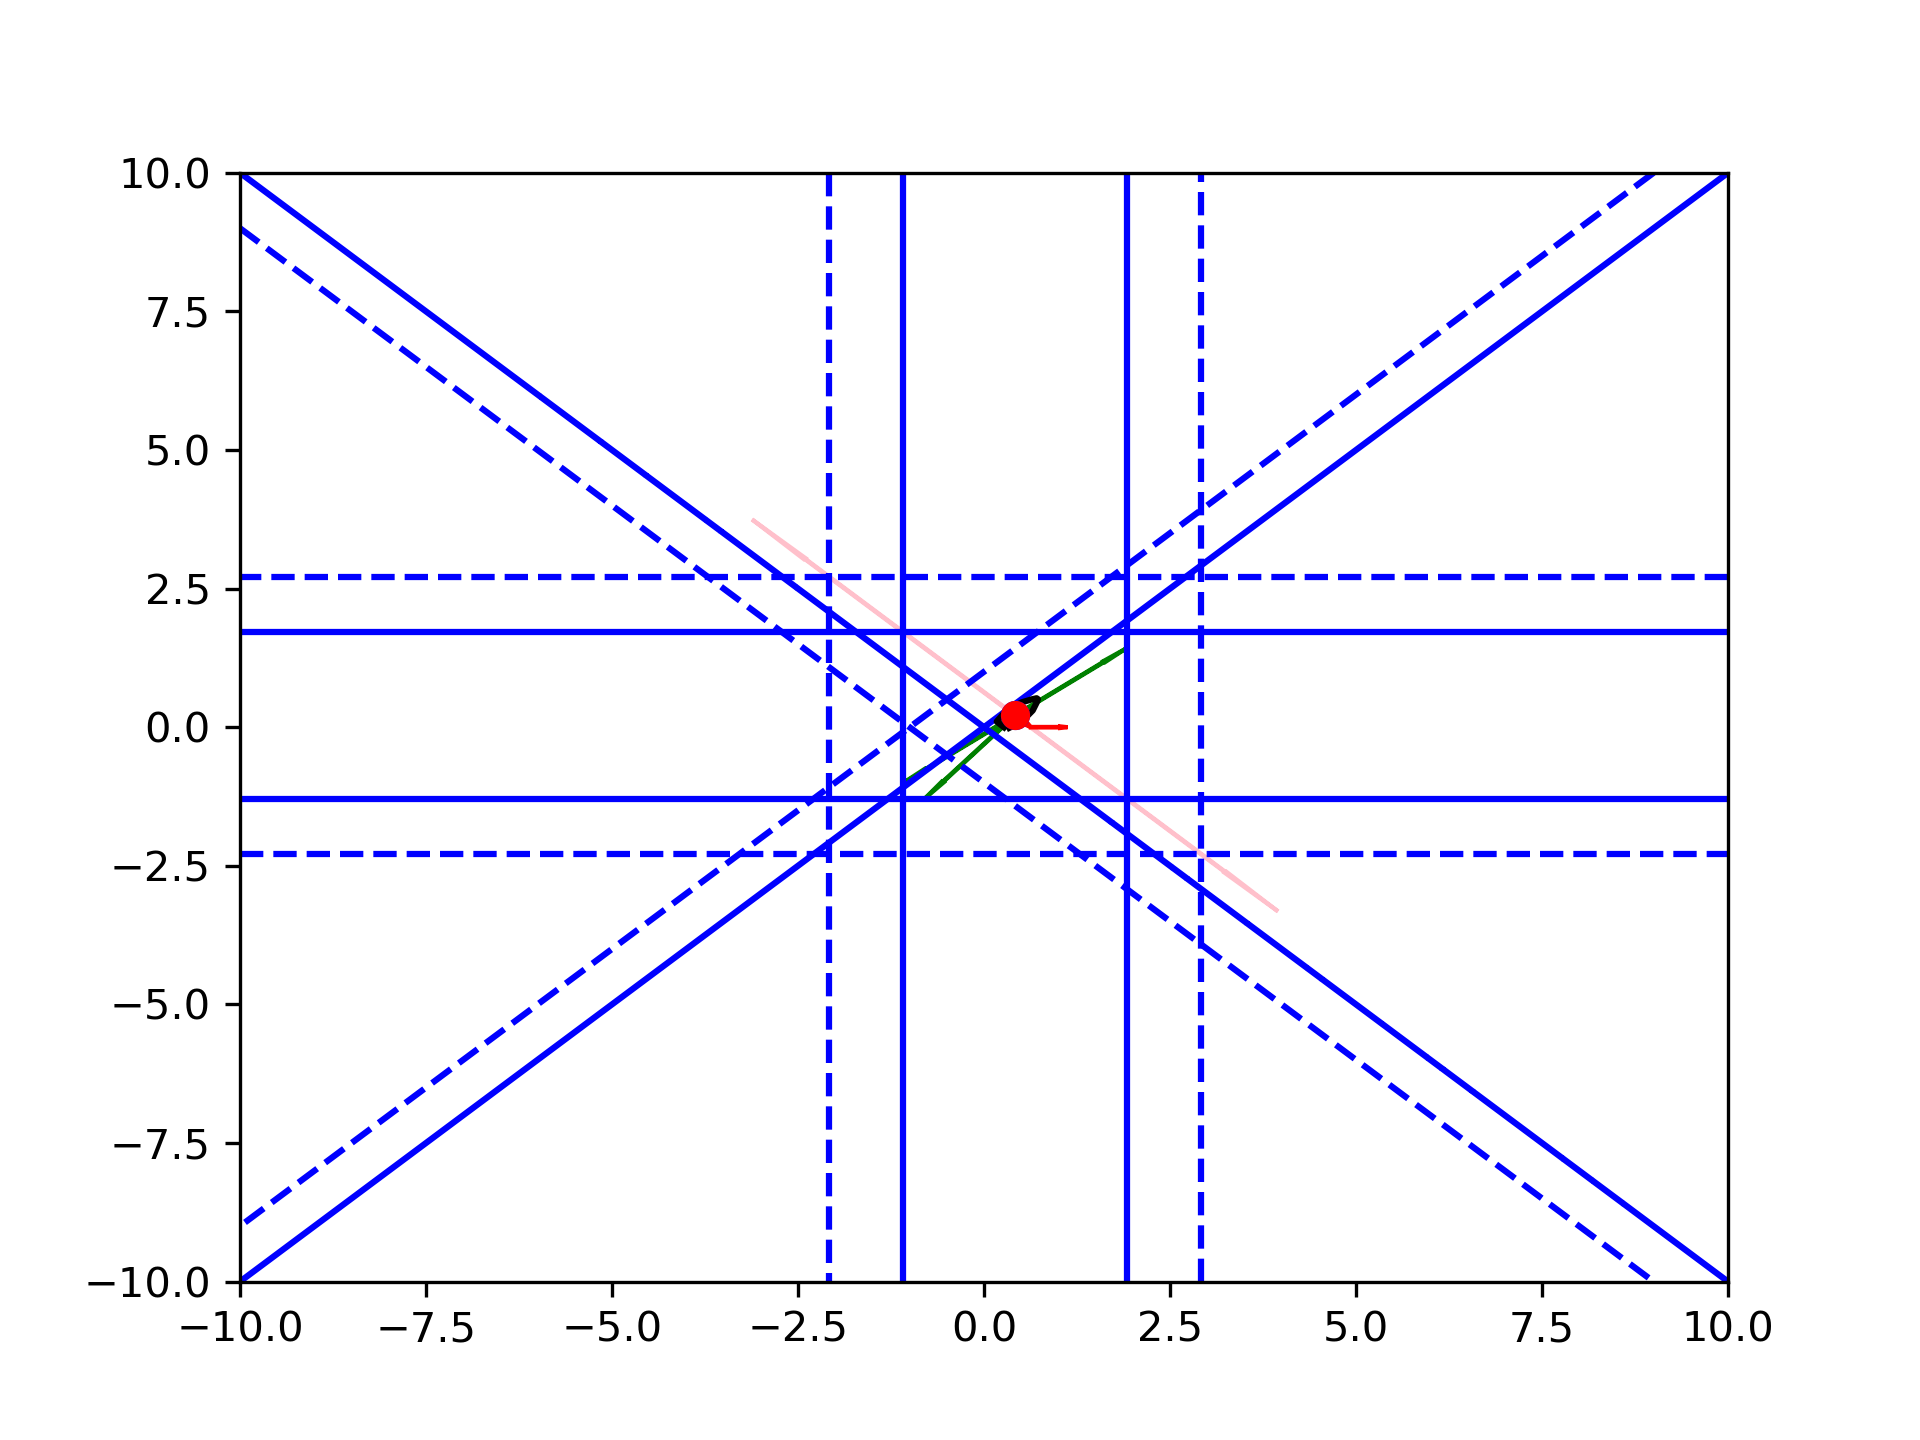
\includegraphics[scale=0.4]{images/run_away_1.png}
    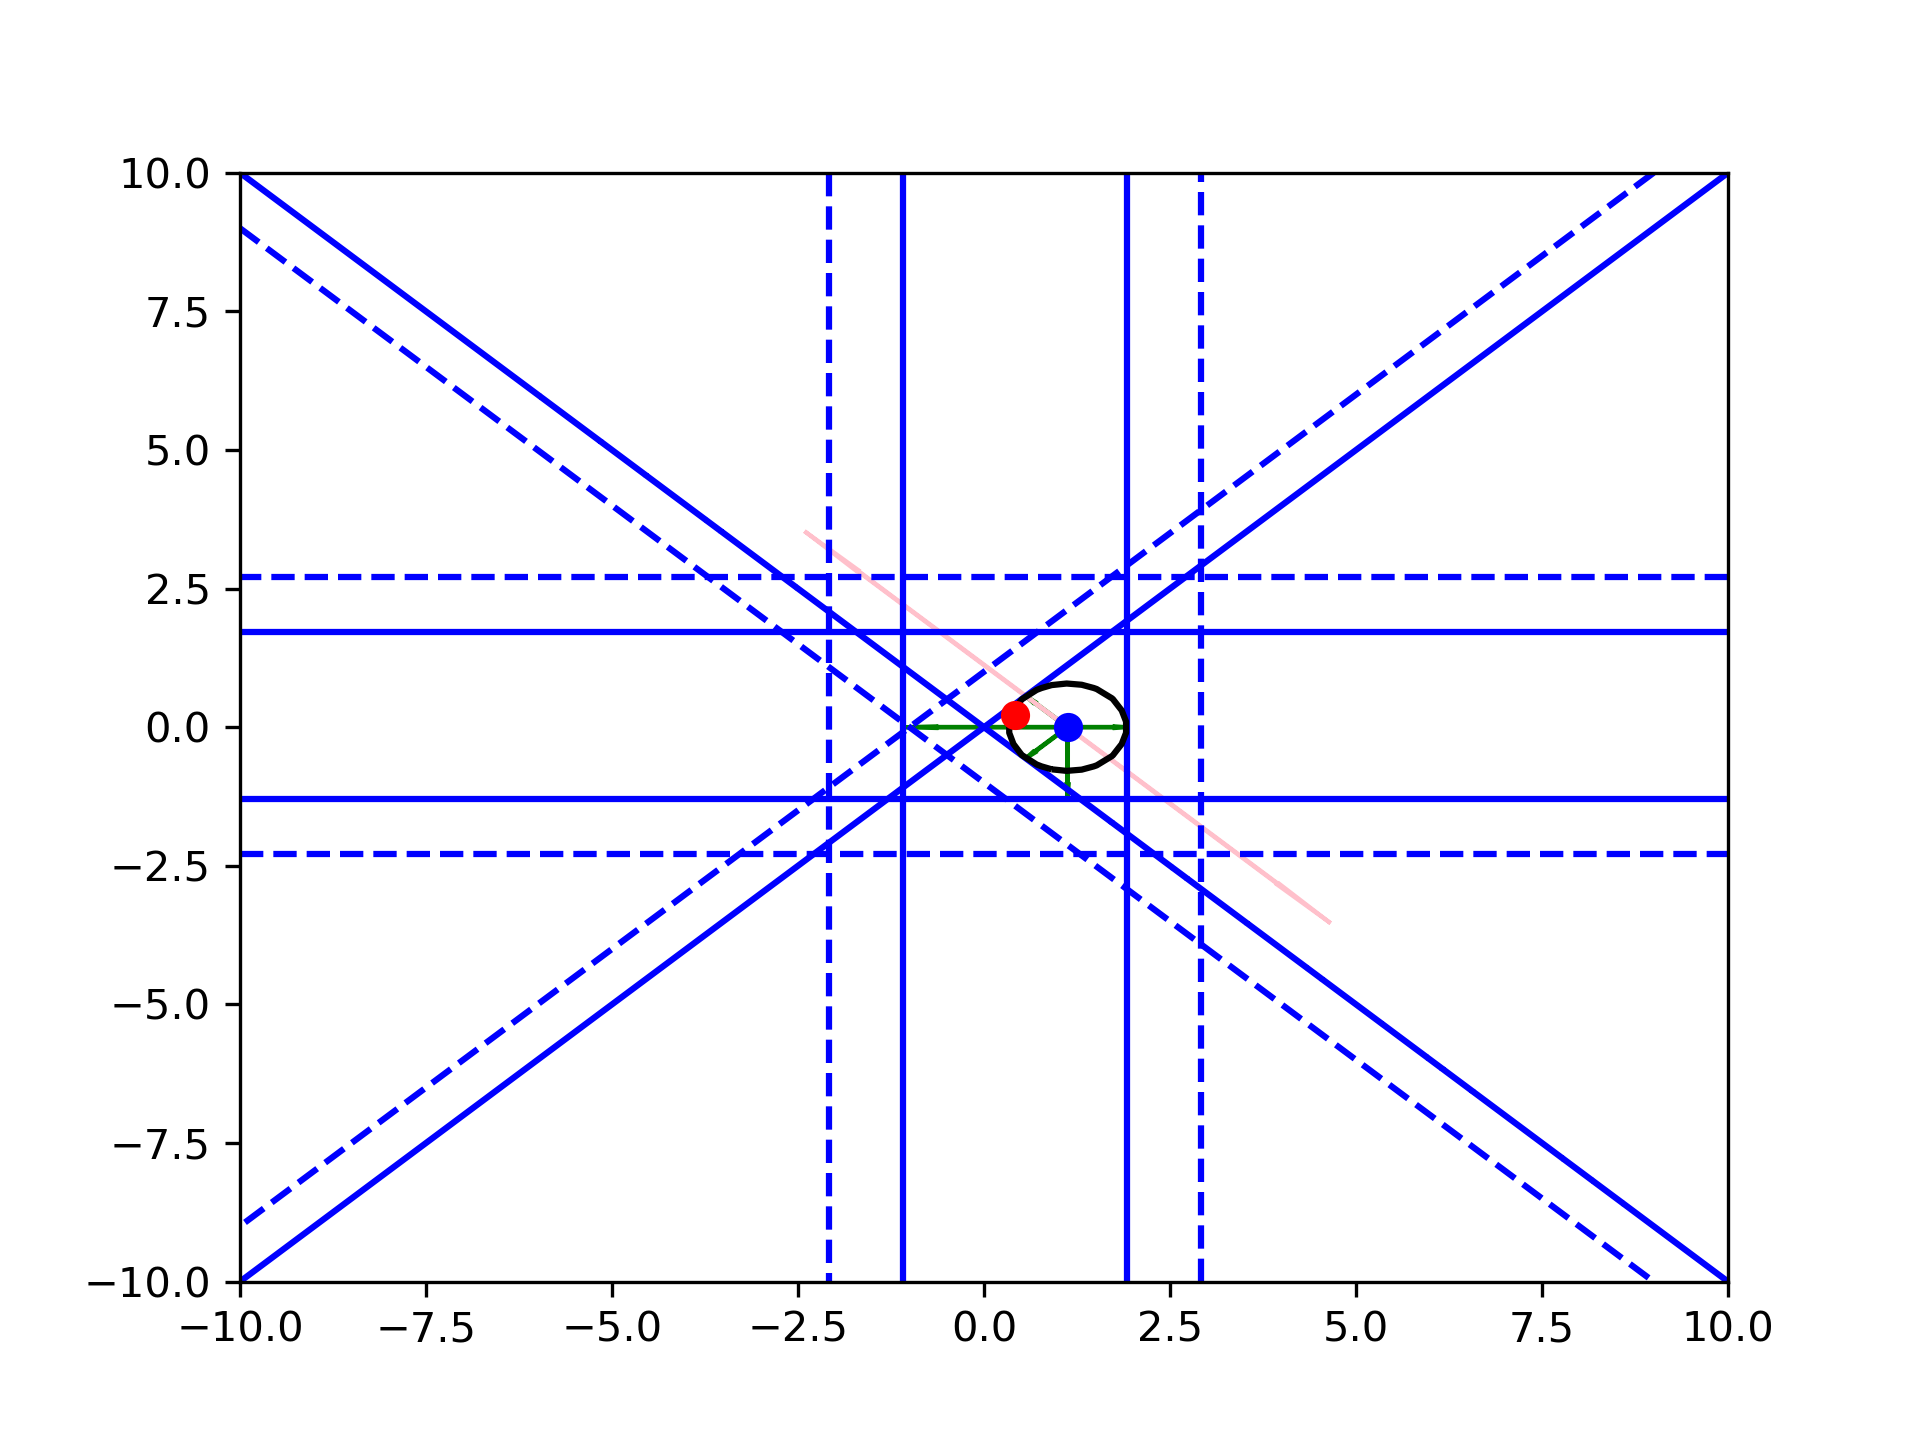
\includegraphics[scale=0.4]{images/run_away_2.png}
    \caption{Ellipse runs away from the optimizer}
    \label{line_can_run}
\end{figure}




\section{Convergence Discussion}
\label{convergence_discussion}

If the tolerances $\tau_{\chi} = 0$ and $\tau_{\Delta} = 0$ are set to zero, the algorithm presented here is a particular implementation of the algorithm presented in \cite{doi:10.1080/10556788.2015.1026968}.
Thus, five hypothesis are required for the convergence analysis:

\begin{itemize}
\item[H0] The trial point during each iterate satisfies the efficiency condition \cref{efficiency}.
\item[H1] The function $f$ is differentiable and its gradient $\nabla f$ is Lipschitz continuous over $\domain$.
\item[H2] The function $f$ is bounded below over $\domain$.
\item[H3] The Hessian's of $f$ are uniformly bounded at each iterate.
\item[H4] The accuracy condition \cref{accuracy}.
\end{itemize}

Hypothesis H1, H2, and H3 are kept as assumptions within our algorithm.
Hypothesis 0 is satisfied by the Generalized Cauchy Point \cite{Conn:2000:TM:357813} if we set $\searchtrk = \outertrk \cap \feasible$ as discussed in \cref{search_a_lot}.
As discussed in \cref{ellipsoidal_lambda}, Hypothesis H4 is satisfied by letting $\sampletrk$ have an ellipsoidal shape as discussed within \cref{bluepill} as long as the condition number of $\qk$ is bounded.

However, we must ensure that we are always able to find a feasible ellipsoid.
Although it is not always possible to find a feasible ellipsoid that contains the current iterate,
we can find a feasible ellipse that needs only be scaled by a constant to do so.
It is shown in \cite{Billups_Larson_2013} that a lambda poised set over a sphere remains lambda poised over a larger sphere (with a larger lambda).

The following proof shows that such a feasible ellipse exists, and provides the required equations for constructing the ellipse.

\begin{theorem}
Given a polyhedron $P = \{x | Ax \le b \}$, where the rows of $A$ are linearly independent, and a point $\xk \in P$,
there exists an ellipsoid $E = \{x | (x - c)^TQ(x - c) \le \frac 1 2 \epsilon \}$ within the polyhedron $E \subset P$,
such that $(\xk - c)^TQ(\xk - c) \le \epsilon$.
Furthermore, letting $\mathcal A(x) = \{1\le i\le n | A_ix = b_i\}$, $
\alpha = \max_{x \in P, i \in \mathcal A(x)} -A_i\frac{A_{\mathcal A}^T(A_{\mathcal A}A_{\mathcal A}^T)^{-1} e}{\|A_{\mathcal A}^T(A_{\mathcal A}A_{\mathcal A}^T)^{-1} e\|}$ we have that

\begin{align*}
\sigma(Q) = \frac{\max\{1, \alpha^{-2}\}}{\min\{1, \alpha^{-2}\}}.
\end{align*}

\end{theorem}

\begin{proof}
Assume without loss of generality that $A$ and $b$ have been normalized so that $\|A_i\| = 1$.
Let $\mathcal A$ be the set of active constraints at $\xk$: $\mathcal A = \mathcal A(\xk) = \{ i | A_i\xk = b_i\}$.
If $\mathcal A = \emptyset$, then we are free to select $c = \xk, Q = I$, and $ \epsilon $ sufficiently small.
Otherwise, compute $u = -A_{\mathcal A}^T(A_{\mathcal A}A_{\mathcal A}^T)^{-1} e$, $\hat u = \frac {u} {\| u\|} $, $\alpha = -\max_{i \in \mathcal A} A_i \hat u$, and define the cones
\begin{align}
C_1 = \{x \in \mathbb R^n | \quad x = \xk + t\hat u + s, s^T\hat u = 0, t > 0, \|s\| \le \alpha t\} \label{s_less_t} \\
C_2 = \{x = (t, s)^T \in \mathbb R^n, t \in \mathbb R, s \in \mathbb R^{n-1} |\quad \|s\| \le a t \}.
\end{align}

First, we show that $C_1$ is feasible with respect to the active constraints at $\xk$,
by letting $y = \xk + t\hat u + s\in C_1$ as in \ref{s_less_t} and $i \in \mathcal A$ be arbitrary.
With these definitions, the active constraints are satisified at $y$:
\begin{align*}
A_{i}y - b_{i} = A_{i}(t\hat u + s) = A_{i}s + t A_{i}n \le \|s\| - \alpha t \le 0.
\end{align*}

Now, for an arbitrary $\delta > 0$, let 
$f(x): \mathbb R^n \to \mathbb R$ be defined by 
\begin{align*}
f(x) = (x - \delta e_1)^T\begin{bmatrix}
1 & \boldsymbol0^T \\
\boldsymbol 0 & \alpha^{-2} \boldsymbol I \\
\end{bmatrix}(x - \delta e_1) - \frac 1 2 \delta^2,
\end{align*} 
and consider the ellipsoid $E_1 = \{x | f(x) \le 0\}$.
We will show that $E_1 \subseteq C_2$.
Letting $t \in \mathbb R$ be arbitrary, we see that
\begin{align*}
2\big(t - \frac {\delta} 2\big)^2 \ge 0
\Longrightarrow 2t\delta - \frac 1 2 \delta^2 \le 2t^2 
\Longrightarrow \frac 1 2 \delta^2 - (t - \delta)^2 \le t^2. 
\end{align*}

% \Longrightarrow \frac 1 2 \delta^2 -t^2  + 2t\delta - \delta^2 \le t^2 \\
% \Longrightarrow 0 \le t^2 - t\delta + \frac 1 4 \delta^2
%  \Longrightarrow 0 \le 2t^2 - 2t\delta + \frac 1 2 \delta^2\\
If we further suppose that $x = (t, s)^T \in E_1$ for some $s \in \mathbb R^{n-1}$, we see that
\begin{align*}
(x - \delta e_1)^T\begin{bmatrix}
1 & \boldsymbol0^T \\
\boldsymbol 0 & \alpha^{-2} \boldsymbol I \\
\end{bmatrix}(x - \delta e_1) \le \frac 1 2 \delta^2 \\
\Longrightarrow (t - \delta)^2 + \frac {1} {\alpha^2} \|s\|^2 \le \frac 1 2 \delta^2 \\
\Longrightarrow \|s\|^2 \le \alpha^2 \big(\frac 1 2 \delta^2 - (t - \delta)^2\big) \le \alpha^2t^2\\
\Longrightarrow \|s\| \le \alpha t\\
\end{align*}
so that $x \in C_2$.
Also, note that by scaling the ellipse by a factor of $2$, the ellipsoid

\begin{align*}
\bigg \{x \bigg | (x - \delta e_1)^T\begin{bmatrix}
1 & \boldsymbol0^T \\
\boldsymbol 0 & \alpha^{-2} \boldsymbol I \\
\end{bmatrix}(x - \delta e_1) \le \delta^2 \bigg\},
\end{align*}
includes the origin:
\begin{align*}
(0 - \delta e_1)^T\begin{bmatrix}
1 & \boldsymbol0^T \\
\boldsymbol 0 & \alpha^{-2} \boldsymbol I \\
\end{bmatrix}(0 - \delta e_1) = \delta^2 \le \delta^2.
\end{align*}

All that remains is to translate this ellipsoid by $\xk$ and rotate $\hat u$ into $e_1$ with the rotation matrix $R \in SO(n)$:
\begin{align*}
R = 2\frac{(e_1 + \hat u)(e_1 + \hat u)^T}{(e_1 + \hat u)^T(e_1 + \hat u)} - \boldsymbol I
\end{align*}
which satisfies
\begin{align*}
Re_1 = \hat u, \quad
R\hat u = e_1, \quad
\det(R) = 1.
\end{align*}


Thus, with $Q = R^T\begin{bmatrix}
1 & \boldsymbol0^T \\
\boldsymbol 0 & \alpha^{-2} \boldsymbol I \\
\end{bmatrix}R$, $c = \xk - \delta \hat u$, $\epsilon = \delta^2$ we have constructed a feasible ellipse
\begin{align*}
E_2 = \bigg \{x \bigg | (x - \xk - \delta \hat u)^T\bigg(R^T\begin{bmatrix}
1 & \boldsymbol0^T \\
\boldsymbol 0 & \alpha^{-2} \boldsymbol I \\
\end{bmatrix}R\bigg)(x - \xk - \delta \hat u) \le \frac 1 2 \delta^2 \bigg\},
\end{align*}
for sufficiently small $\delta$, that can be scaled by $2$ to include $\xk$.
Note that the condition number of this matrix is $\sigma(Q) = \frac{\max\{1, \alpha^{-2}\}}{\min\{1, \alpha^{-2}\}}$,
as the condition number is not affected by rotations.
% The value of $\alpha$ only depends on the polyhedron, and is therefore bounded given a problem.


\end{proof}


% \paragraph{}
% While including a center search and only using a sphere for $\sampletrk$ ensures that this will be the case as long as there is an interior point to the feasible region.
% However, for more complicated ellipsoid searches must be able to find an ellipse.
% One strategy that ensures the ellipse can be constructed for all of our ellipse searches is to find an ball containing the current iterate and running a local search optimization routine with this initial ball as input.


% 
% \paragraph{}
% Another strategy is to add a check within the \emph{ConstructTrustRegion} routine that decreases the trust region radius whenever a suitable ellipse is not found.
% The presented convergence analysis will still hold as $S$ can contain only finitely many terms not in $\bar S$.

% \paragraph{}
% \color{red}
% For convex constraints, there will exist a bound on the condition numer of $\qk$ as long as $\outertrk$ is bounded.
% An argument for this might be as follows:
% Maybe, by increasing the outer trust region radius, we can only increase the condition number of $\qk$.
% \color{black}






\section{Introduction}

Derivative free optimization (DFO) refers to mathematical programs involving functions for which derivative information is not explicitly available.
Such problems arise, for example, when the functions are evaluated by simulations or by laboratory experiments.
In such applications, function evaluations are expensive, so it is sensible to invest significant computational resources to minimize the number of function evaluations.

This work is aimed at developing algorithms to solve constrained optimization problems of the form 

\[ \begin{array}{ccl} \min_{x \in \domain} & f(x) \\
\mbox{subject to} & c_i(x) \le 0 & i \in \mathcal{I} \\
& c_i(x) = 0 & i \in \mathcal{E},
\end{array}
\]
where $\domain$ is a subset of $\real^n$, and $f$ and $c_i, i \in \mathcal{I} \cup \mathcal{E}$ are real-valued functions on $X$ with at least one of these functions being a {\em black-box} function, meaning that derivatives cannot be evaluated directly.

%%%%%%%%%%%%%%%%%%%%%%%%%%%%%%%%%%%%%%%%%%%%%%%%%%%%%%%%%%%%%%%%%%%%%%%%%%%%%%%%%%%%%%%%%%%%%%%%%%%%%%%%%%%%%%%%%%%%%%%%%%%%%%%%%%%%
% We consider two variations of this problem.
% In the first variation, we assume that the constraints are fully quantifiable.
%%%%%%%%%%%%%%%%%%%%%%%%%%%%%%%%%%%%%%%%%%%%%%%%%%%%%%%%%%%%%%%%%%%%%%%%%%%%%%%%%%%%%%%%%%%%%%%%%%%%%%%%%%%%%%%%%%%%%%%%%%%%%%%%%%%%
As in \cite{DUMMY:typesofconstraints}, partially quantifiable means that all of the functions can be evaluated at any point in $X$ and that the values returned for the constraint functions provide meaningful information about how close the point is to a constraint boundary.
We assume that the black-box functions return meaningful numerical values only when evaluated at feasible points. In this case, the constraints are called {\em partially quantifiable}.   

We are interested in developing {\em model-based} trust-region algorithms for solving these problems.
Model-based methods work by constructing model functions to approximate the black box functions at each iteration.
The model functions are determined by fitting previously evaluated function values on a set of sample points.
In trust-region methods, the model-functions are used to define a trust-region subproblem, whose solution determines the next iterate.
For example, the trust-region subproblem might have the form

\[ \begin{array}{ccl} \min_{\norm{s} \le \Delta_k}
 & \modelk (\iteratek+s) \\
\mbox{subject to} & \modelconstrainti(\iteratek + s) \le 0 & i \in \mathcal{I} \\
& \modelconstrainti(\iteratek + s) = 0 & i \in \mathcal{E},
\end{array}
\]
where $\iteratek$ is the current iterate, $\modelk$ is the model function approximating $f$,  and $\modelconstrainti$ are the model functions approximating the constraint $c_i \forall i \in \mathcal{I} \union \mathcal{E}$, and $\Delta_k$ is the radius of the trust-region.
The key differences between this problem and the original is that all functions are replaced with their model functions, and a trust region constraint has been added.
Conceptually, the model functions are ``trusted'' only within a distance $\Delta_k$ of the current iterate $\iteratek$; so the trust-region subproblem restricts the length of step $s$ to be no larger than $\Delta_k$.
To ensure that the model functions are good approximations of the true functions over the trust region, the sample points are typically chosen to lie within, or at least near, the trust-region.
In our work, we require all sample points to be within the trust region.


An important consideration in fitting the model functions is the ``geometry'' of the sample set.
This will be discussed in more detail in Section \ref{geometry}, but the key point is that the relative positions of the sample points within the trust region have a significant effect on the accuracy of the model functions over the trust region.
When the geometry of the sample set is poor, it is sometimes necessary to evaluate the functions at new points within the trust region to improve the geometry of the sample set.

In the case of partially quantifiable constraints, all of the sample points must lie within the feasible region.
This poses some interesting challenges for the geometry of the sample set.
As a first step toward developing an algorithm to solve such problems, we consider a simplified problem where all of the constraints are linear, but we impose the restriction that all sample points must lie within the feasible region.

%%%%%%%%%%%%%%%%%%%%%%%%%%%%%%%%%%%%%%%%%%%%%%%%%%%%%%%%%%%%%%%%%%%%%%%%%%%%%%%%%%%%%%%%%%%%%%%%%%%%%%%%%%%%%%%%%%%%%%%%%%%%%%%%%%%%
% In the case of fully quantifiable constraints, there is no difficulty in using sample points outside of the feasible region.  
% In Chapter \ref{chap:Filter}, we describe a Trust-Region SQP Filter method for solving this class of problems.
%%%%%%%%%%%%%%%%%%%%%%%%%%%%%%%%%%%%%%%%%%%%%%%%%%%%%%%%%%%%%%%%%%%%%%%%%%%%%%%%%%%%%%%%%%%%%%%%%%%%%%%%%%%%%%%%%%%%%%%%%%%%%%%%%%%%
  

\subsection{Always Feasible Motivation}

Algorithms that maintain feasibility in both the iterates and sample points provide some useful qualities.
Firstly, they are able to solve problems with \emph{partially-quantifiable} constraints.
One scenario in which partially-quantifiable constrains may arise is within the problem of minimizing an expensive simulation.

%\begin{center}
%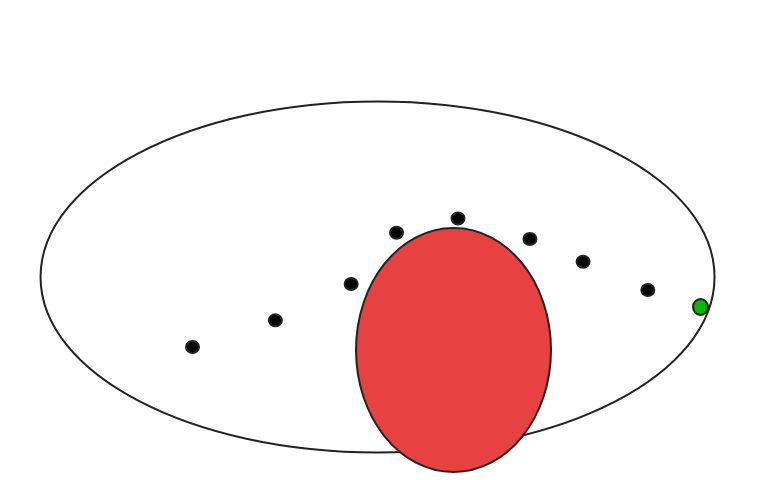
\includegraphics[width=200px]{images/infeasible_constraint.png}
%\end{center}

If the runtime of the simulation depends on its inputs, and the simulation is not allowed to finish when a runtime threshold is met, the runtime will force some inputs to be infeasible.
However, when the simulation does complete, its runtime is quantifiable, and can be used to construct a model of the infeasible region.
An algorithm that wishes to minimize this simulation is forced to account for this constraint.


Additionally, an always feasible algorithm is also an \emph{any-time} algorithm.
Anytime algorithms are a class of algorithms that can conveniently be run as long as desired and return the best solution found so far if interrupted.
These algorithm are of practical importance when problems have encertain time complexity.


\section{Derivative Free Background}
% 
% \subsection{Strategy}
% A reasonable approach to DFO is to modify classical algorithms that rely on derivatives by using the derivatives of the model functions whenever a derivative is needed in the algorithm.
% However, the lack of explicit derivatives pose several challenges, which necessitate changes in the classical algorithms.
% First, care must be taken to ensure that the model functions are sufficiently accurate approximations to the true functions.
% This means that geometry of the sample points must be considered.
% It also means that the trust-region radius must get arbitrarily small.
% 
% The transition to the derivative-free setting also provides some interesting research opportunities.
% In particular, because function evaluations are so costly, there is potential for significant gains by considering more complex optimization paradigms.
% For example, Sequential Quadratic Programming (SQP) methods use subproblems involving quadratic approximations of the objective function $f$ and linear approximations of the constraint functions.
% In the derivative-free setting, it may be worthwhile to explore other variations of the classical algorithms.
% For example, it might be worthwhile to construct quadratic models of the constraint functions, which might result in fewer iterations overall.
% 
% It might also be worthwhile to consider using different sample sets for fitting different functions.  
% For example, the SQP trust-region filter method involves constructing a quadratic model of the objective function and linear models of the constraint functions.  But this raises an interesting question, since a good sample set for constructing a quadratic model may not be ideal for fitting the linear functions modeling the constraints.  

\subsection{Recent Work}
\paragraph{Applications}
Recently, there has been a growth in applications of derivative free optimization.
Such applications include photinjector optimization \cite{1742-6596-874-1-012062}, circuitry arrangements \cite{PLOSKAS201816}, machine learning \cite{KS2018}, volume optimization \cite{Cheng2017}, and reliability based optimization \cite{Gao2017}.

\paragraph{Constrained derivative free algorithms}
To address the rise in these applications, new algorithms are being developed such as \cite{doi:10.1080/10556788.2015.1026968} which is an algorithm similar to the one presented here, but the sample points are not always feasible.
\cite{Tröltzsch2016} presents another similar algorithm for equality based constraints.
\cite{infeasiblestarting} presents an algorithm which accepts an infeasible starting point.
\cite{Gao2018} also presents an algorithm for linearly constrained derivative free optimization that uses a backtracking technique to minimize the number of evaluations required.

\paragraph{Subproblems}
Some work has been done within trust region algorithms to improve the update policy \cite{Kamandi2017}.
Also, \cite{Verdério2017} and \cite{doi:10.1080/10556780802409296} discuss geometric conditions of the sample points required for global convergence.
Finally, \cite{AMAIOUA201813} uses a mesh adaptive search to solve quadratic subproblems.


\paragraph{Complexity Analysis}

A derivation is found in \cite{doi:10.1137/151005683} which shows that to driver the norm of the gradient less than $\epsilon$, the number of function evaluations can be bounded by $O(\epsilon^{-2})$ 
%and $O(n^2\epsilon^{-2})$ 
function evaluations for derivative free model based approaches. Also, cubic over estimation with finite differences can acheive $O(\epsilon^{-1.5})$. \cite{doi:10.1093/imanum/drx043} is another recent paper presenting complexity analysis using probabilistic methods.


\paragraph{Reviews}
Within \cite{DUMMY:intro_book} derivative-free methods are developed in detail.
This is the first text book devoted to derivative free optimization.
It contains a good explanation of ensuring geometry of the current set with poisedness for unconstrained problems and also covers other derivative-free methods including direct-search and line search.

A good review of derivative free algorithms and software libraries can be found in \cite{DUMMY:review}.
This compares several software libraries, and reviews the development of derivative free optimization since it started.
Another recent review can be found in \cite{DUMMY:review2}.

% TODOOOOOOOOOOOOOOOOOOOOOOOOOOOOOOOOOOOOOOOOOOOOOOOOOOOOOOOOOOOOOOOOOOOOOOOOOOOOOOOOOOOOOOOOOOOOOOOOOOOOOOOOOOOO
% READ THIS

\subsubsection{Sampling issues}
Derivative free trust region algorithms can choose sampling points to construct their model functions.
When this is done, care must be taken to avoid issues with two important aspects: their \emph{geometry} and \emph{proximity}.

\paragraph{Interpolation}
\label{geometry}
The term \emph{geometry} describes how the ``shape" of any $p+1$ sample points $Y = \{y^0, y^1, \ldots, y^p\}$ affects the model's accuracy.
We desire a method to choose new sample points that provides error bounds on not only the function values, but also on several orders of derivatives in some region around the current iterate.
The model is constructed to agree with the original functions on at least the sample points: we evaluate the objective here, so that we know the true function values at these points.
For the objective, this becomes
\begin{align}
\label{interpolation_condition}
\modelk(y^i) = f(y^i) \quad \forall \quad 0 \le i \le p.
\end{align}
This is known as the \emph{interpolation condition}.

It is convenient to write the model as a linear combination of basis polynomials $\{\phi_0, \phi_2, \ldots, \phi_p\}$.
To satisfy the interpolation condition \ref{interpolation_condition}, we then chose this linear combination by selecting coefficients $\alpha_0, \ldots, \alpha_p$ to satisfy
\[
    \modelk(y^i) = \sum^p_{j=0}\alpha_j\phi_j(y^i) = f(y^i) \quad \forall \quad 0 \le i \le p.
\]

We can also write this equation in matrix form.
If we define the Vandermode matrix as
\begin{align}
\label{vandermonde}
V=
\begin{bmatrix}
    \phi_1(y^0)      & \phi_2(y^0)       & \ldots & \phi_{p}(y^0)      \\
    \phi_1(y^1)      & \phi_2(y^1)       & \dots  & \phi_{p}(y^1)      \\
                     &                   & \vdots &                    \\
    \phi_1(y^{p})    & \phi_2(y^{p})     & \ldots & \phi_{p}(y^{p})
\end{bmatrix},
\end{align}

the interpolation condition becomes:
\begin{align}
V
\begin{bmatrix}
    \alpha_0     \\
    \alpha_1     \\
    \vdots       \\
    \alpha_p
\end{bmatrix}
=
\begin{bmatrix}
    f(y^0)     \\
    f(y^2)     \\
    \vdots     \\
    f(y^p)
\end{bmatrix}
\end{align}

\paragraph{Geometry}
This system has a unique solution if and only if $V$ is nonsingular, so that we are able to solve this system of equations to determine our model functions.
However, even when $V$ is nonsingular but ``close" to singular, as measured by its condition number, the model's approximation may become less accurate.
% The condition number of $V$ measures how far the current Vandermode matrix is from being illpoised.
Algorithms must be careful to avoid choices of sample points $Y$ that cause the condition number of this matrix to be poor.

This system becomes trivial after a change of basis to the \emph{Lagrange polynomials} for the sample set $Y$.
The Lagrange polynomials $l_0, l_1, \ldots, l_p$ for the sample set $Y$ are set of lowest degree polynomials such that
\[
l_i(y^j) = \delta_{i,j}
\]
where $\delta_{i,j} = \{0 \;\text{if}\; i\ne j,\quad 1 \;\text{if} \; i = j $ is the Kronecker-delta function defined in table \ref{tab:TableOfNotation}.
For example, after this change of basis, note that the Vandermode matrix becomes the identity matrix.
Thus, we can conveniently write
\[
\label{reg}
\modelk(x) = \sum^p_{j=0}f(y^i)l_i(x).
\]
Note that this implies computing the change of basis to the Lagrange polynomials amounts to inverting this Vandermode matrix.
This relationship allows us to use properties of the Vandermode matrix and these lagrange polynomials to find conditions on our sample points that ensure nice geometry.

In particular, we say that a set $Y$ is $\Lambda$-poised for a fixed constant $\Lambda$ with respect to a bases $\phi$ on the ball 
$B_2(0, 1)$ (defined in table \ref{tab:TableOfNotation}) if and only if for the lagrange polynomials $l_i$ associated with $Y$
\begin{align}
\Lambda \ge \max_{0\le i\le p}\max_{x\in B_2(0, 1)}|l_i(x)|
\end{align}

This can be shown to be equivalent to the following condition \cite{DUMMY:intro_book}.
For any $x \in B_2(0, 1)$ there is a $\lambda \in \mathbb R ^ {p+1}$ such that 
\begin{align}
\sum_{i=0}^p\lambda_i\phi_i(y^i) = \phi(x) \\
\|\lambda\|_{\infty} \le \Lambda.
\end{align}

This ensures that the Vandermonde matrix is well conditioned.
Note that in practice, the sample points are shifted by $y^0$.
In fact, if we assume that $f$ is continuously differentiable in an open domain containing $B_2(y^0, \Delta)$ and is Lipschitz continuous, and restrict ourselves to quadratic interpolating functions we have the following results for any $y \in B_2(y^0, \Delta)$:
\begin{align}
 \|f(y) - \modelk(y)\| \le \kappa_{ef} \Lambda \Delta^3 \\
 \|\nabla f(y) - \nabla \modelk(y)\| \le \kappa_{eg} \Lambda \Delta^2 \\
 \|\nabla^2 f(y) - \nabla^2 \modelk(y)\| \le \kappa_{eh}\Lambda \Delta \\
\end{align}
where
$\kappa_{ef}, \kappa_{ef}$, and $\kappa_{ef}$ are constants depending only on the dimension and Lipschitz constant of $f$.

%used to find the coefficients $\lambda$ to express the model function in terms of a basis of Lagrange polynomials $l_i$
Problems become apparent when comparing the Lagrange polynomials associated with a poised set with those of an ill poised set.

In figure \ref{pvip}, a set of quadratic polynomials used to interpolate the function $f(x) = 5 + x + y + (x + y) ^ 2 - \frac 1 {250} y ^ 4$.
We can see that the difference between the model and $f$ are much larger when the points are chosen to be nearly colinear resulting in a much higher $\Lambda$.

\begin{figure}[h]
    \centering
    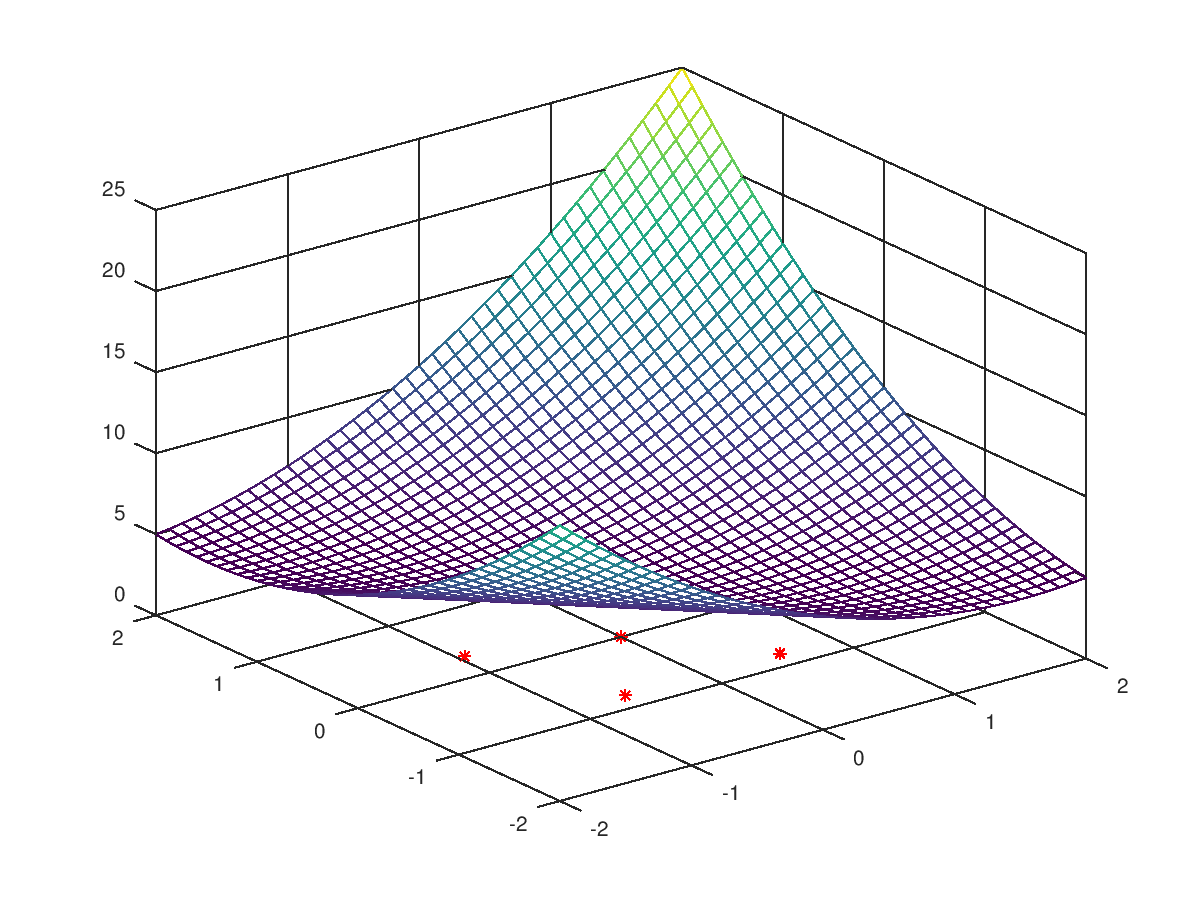
\includegraphics[width=200px]{images/poised_good.png}
    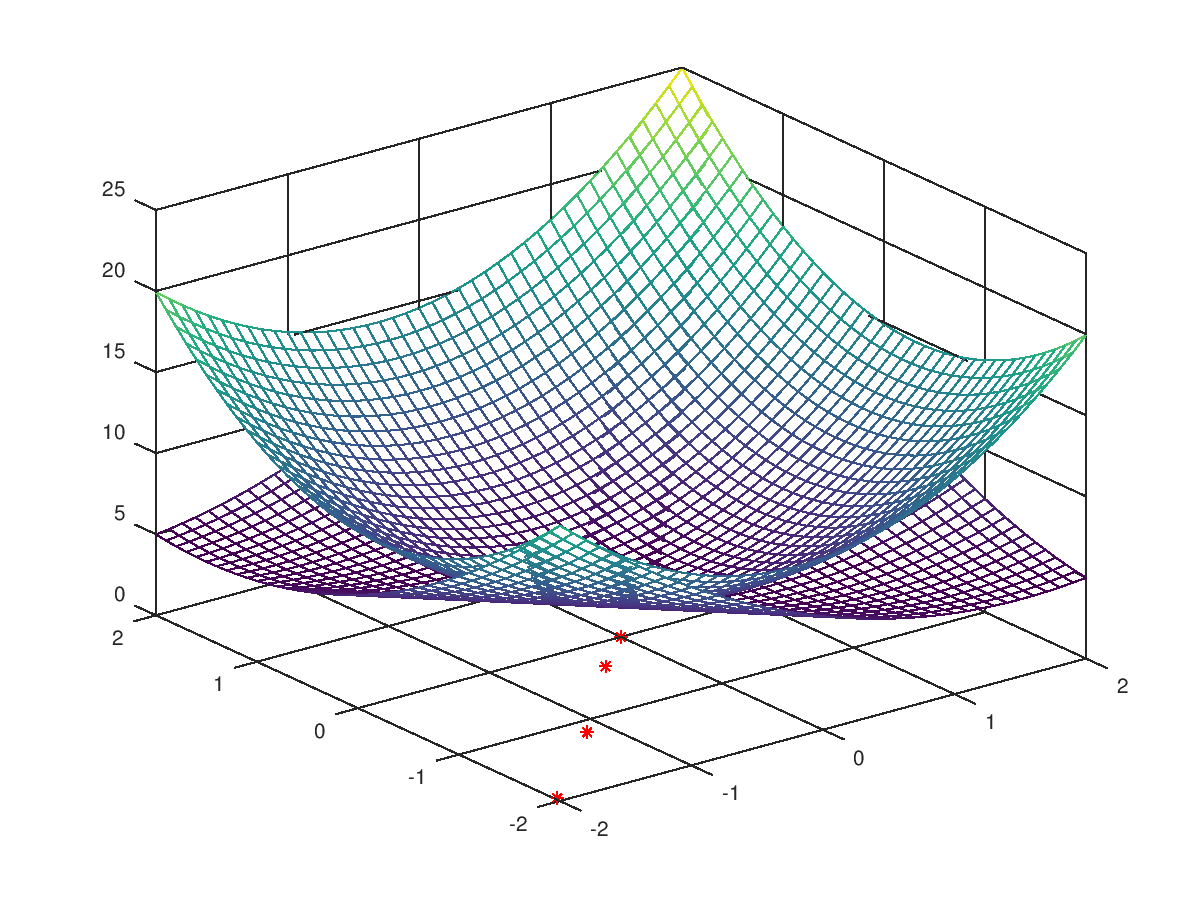
\includegraphics[width=200px]{images/poised_bad.png}
    \caption{Poised vs Ill poised}
    \label{pvip}
\end{figure}


\begin{center}

\end{center}

A more detailed discussion can be found in \cite{doi:10.1080/10556780802409296}, but a step to ensure geometry is required for convergence analysis although it may come at the expense of function evaluations.

\paragraph{Proximity}

Proximity refers to the trust region radius.
The trust region must go to zero if we are to be sure that we have reached a critical point.
In general, the smaller the trust region, the closer to linear or quadratic the original function will look.
This is because the model's error term given is proportional to the trust region radius.

In classical trust region algorithms, there is no need for the trust region radius to go to zero.
Therefore, extra care must be taken to ensure this while modifying these algorithms.

\subsubsection{Assessing model accuracy and radius management}

Each iteration that evaluates a trial point must also test the accuracy of the model functions.
To perform this test, we calculate a quantity
\begin{equation}
\label{rho}
\rho_k = \frac{f(\iteratek) - f(\iteratek+\trialk)}{\modelk(\iteratek) - \modelk(\iteratek+\trialk)}
\end{equation}
which measures the actual improvement over predicted improvement.
A small $\rho$ implies the model functions are not sufficiently accurate, while a large implies that progress torwards minimizing the objective.
This has been widely used within trust region frameworks such as \cite{Conn:2000:TM:357813} and within a derivative free context \cite{DUMMY:intro_book}.
Generally speaking, fixed constants $0 < \gamma_1 \le \gamma_2 \le 1$ and $0 < \omega_{\text{dec}} < 1 \le \omega_{\text{inc}}$ are supplied by the user and determine the trust region update policy.
The update policy frequently follows the following pattern:

\begin{algorithmic}
\If{$\rho < \gamma_1$}
    \State $\iteratekpone \gets \iteratek$ (reject)
    \State $\Delta_{k+1} \gets \omega_{\text{dec}} \Delta_k$
\ElsIf{$\gamma_1 \le \rho \le \gamma_2$}
    \State $\iteratekpone\gets \gets \iteratek + \trialk$ (accept)
    \State $\Delta_{k+1} \gets \omega_{\text{dec}} \Delta_k$
\ElsIf {$\rho > \gamma_2$}
    \State $\iteratekpone \gets \iteratek + \trialk$ (accept)
    \If
        \State $\Delta_{k+1} \gets \omega_{\text{dec}} \Delta_k$
    \Else
        \State $\Delta_{k+1} \gets \omega_{\text{inc}} \Delta_k$
    \EndIf
\EndIf
\end{algorithmic}


\subsection{Model-based Trust Region Methods}

We will be modifying the following classical, trust region algorithm.
%A set of poised points are chosen for some radius $\Delta_k>0$ about the current iterate.
The objective value and derivatives are evaluated at the current iterate to construct its function.
Next, this model function is minimized over the trust region and the minimum argument becomes the trial point.
The objective is evaluated at the trial point and a measure of reduction $\rho$ is computed.
If $\rho$ implies that sufficient reduction has been made and that the model approximates the function well, the trial point is accepted as the new iterate.
Otherwise, the trust region is reduced to increase model accuracy.


For unconstrained optimization, the algorithmic framework can be described with these steps:

\begin{enumerate}
	\item Create a model function $\modelk(x)$.
	\begin {itemize}
		\item In classical trust region methods, the following quadratic model function is used:
		\[
		\modelk(x) = f(\iteratek) + \nabla f(\iteratek)^T (x-\iteratek) + \frac 1 2 (x-\iteratek)^T\nabla^2f(\iteratek)(x-\iteratek)
		\]
	\end{itemize}
	%\begin{itemize}
		% \item $\nabla f(\iteratek)$ and $\nabla^2 f(\iteratek)$ must be approximated
		%\item Geometric properties of the sample set must be satisfied
	%\end{itemize}
	
	\item If $\nabla f(\iteratek) < \tau$ stop, where $\tau$ is some tolerance
	
	\item Solve the Trust region subproblem: $s^{(k)} = \argmin_{s\in B_2(0; \Delta_k)} \modelk (\iteratek + s)$ where $B_2$ is the ball of radius $\Delta_k$ defined in table \ref{tab:TableOfNotation}.
	
	\item Test for improvement
	\begin{itemize}
		\item Compute a measure of model accuracy $\rho$ see \ref{rho}
		\item If $\rho$ is small, $\iteratekpone=\iteratek$ (reject) and decrease radius
		\item If $\rho$ is intermediate, $\iteratekpone=\iteratek+\trialk$ (accept) and decrease radius
		\item If $\rho$ is large, $\iteratekpone=\iteratek+\trialk$ (accept) and either increase the radius or decrease if $\nabla \modelk(\iteratek)$ is small
	\end{itemize}
	
	\item Go to step 1
\end{enumerate}

Our goal is to generalize this framework to handle constraints, where we must ensure no constraint violation while ensuring the accuracy of the models of the constraints.
Two challenges while adopting this framework to derivative free optimization are
\begin{enumerate}
    \item Taylor approximations are not available
    \item We must ensure $\Delta_k \to 0$
\end{enumerate}
Because explicit derivatives are not available, Taylor approximations cannot be used.
The alternative to Taylor approximations that we employ is interpolation.
Also, classical trust region methods do not require $\Delta_k \to 0$, but the bounds on model accuracy in derivative free optimization depend on the trust region radius.
This means that in order to ensure $\nabla f < c\tau$ using the approximation  $\nabla \modelk < \tau$, the trust region must be sufficiently small.
  
%\subsection{Constrained DFO}
%Derivative free optimization problems can be broken into several categories based on the form of functions within the program.
%Several of these categories are described nicely in \cite{DUMMY:typesofconstraints}.
%For example, a typical constrained program within DFO is given by:
%\[ \begin{array}{ccl} \min & f(x) \\
%\mbox{subject to} & c_i(x) \le 0 & i \in \mathcal{I} \\
%& c_i(x) = 0 & i \in \mathcal{E}
%\end{array}
%\]
%where at least one of the functions $f, c_i, i \in \mathcal{I} \cup \mathcal{E}$ is a black box function,
%meaning that we have no information about its derivatives.
% If $c(x, S(x)) = c(x)$, then 

%A well studied case is when the derivatives of $c$ are known, so the objective is the only derivative free function.
%For example, there several libraries exist for Box Constrained DFO (BCDFO) where the constraints take the form $b_{L} \le x \le b_{U}$ for some $b_{L} < b_{U}$.
%However, the problem becomes more difficult in our case where no derivative information of $c$ or $f$ is known.






















%\paragraph{Types of constraints}
%%Regression based methods work by evaluating model functions on a set of sample points to construct local models of the functions.
%%This at least allows the algorithm to minimize these easier model functions over a trust region, rather than working with the original function.

%One distinction important to the choice of sample points is fully quantifiable constraints versus partially-quantifiable constraints.
%If the constraints are fully quantifiable, they can be evaluated anywhere and present no restriction to the sample points.
%However, partially-quantifiable constraints only produce meaningful values within the feasible region.

%If the constraints are fully-quantifiable, a trust-region filter method can be used.
%We describe this approach in \ref{}.
%When the constraints are partially-quantifiable, the goal is to modify the trust region to avoid evaluating the simulation function outside of the feasible region.
%This is described in \ref{}.
%
%For the first step towards developing this algorithm, we develop develop an algorithm that uses linear constraints to model a linearly constrained region.
%This is described in \ref{feasiblemethod}





%We work within a trust region, sequential quadratic programming framework with interpolating model functions.
%For our algorithm, we assume that all functions are derivative-free: all functions are evaluated by a single call to a black box function:
%$S(x) = (f(x), c_{\mathcal {I}}(x)^T, c_{\mathcal {E}}(x)^T)^T$.

%\color{blue}
%We also assume that we are not able to evaluate points outside the feasible region.
%This introduces a new type of constraint: it is not quite a hidden constraint because we do observe function values within the feasible region.
%However, it does implies similar difficulty to construct the model function near the boundary of the feasible region because we have limited sampling ability.
%\color{black}
%\color{red}

%\subsubsection{Interpolation/regression models}
%Within interpolation model-based methods, we construct our model by regressing basis functions onto a set of sampled points.
%For example, given a function $f(x) : \mathbb R^n \to \mathbb R$ we can use a set of basis functions $\phi_i : \mathbb R^n \to \mathbb R \quad \forall 1 \le i \le d_1$ to %construct a model function $m(x) = \sum_{i=1}^{d_1} \lambda_i \phi_i(x)$ approximating $f(x)$ by selecting appropriate $\lambda_i \in \mathbb R$.
%This is done by choosing a set of sample points
%$Y = \{y^1, y^2, \ldots, y^{d_2}\}$,
%evaluating $f = (f_1 = f(y^1), f_2 = f(y^2), \ldots, f_d = f(y^{d_2}))^T$
%and forcing model agreement with the original function $f(x)$ by ensuring

%\begin{equation}
%\label{reg}
%\begin{bmatrix}
%    \phi_1(y^1)      & \phi_2(y^1)       & \ldots & \phi_{d_1}(y^1)      \\
%    \phi_1(y^2)      & \phi_2(y^2)       & \dots  & \phi_{d_1}(y^2)      \\
%                     &                   & \vdots &                      \\
%    \phi_1(y^{d_2})  & \phi_2(y^{d_2})   & \ldots & \phi_{d_1}(y^{d_2})
%\end{bmatrix}
%\begin{bmatrix}
%    \lambda_1      \\
%    \lambda_2      \\
%    \vdots         \\            
%    \lambda_{d_1}
%\end{bmatrix}
%\approx
%\begin{bmatrix}
%    f_1      \\
%    f_2      \\
%    \vdots         \\            
%    f_{d_2}
%\end{bmatrix}.
%\end{equation}

%The matrix on the left hand side is called the Vandermonde matrix defined in \ref{vandermonde} and the set $y^i, i=1\ldots d_2$ are the sample points.
%When $d_1 = d_2$ this is called interpolation and equality is desired within \ref{reg}.
% It could be important to discusss this, because we may use different orders for the constraints than the objective.
%When $d_1 < d_2$ this is called underdetermined interpolation, 
%This can be handled by requesting and a minimum norm solution.
%Finally, when $d_1 > d_2$ this is called regression and only a least squares solution can be requested.
%Note that in practice, the set $Y$ is shifted and scaled.
%\color{black}


%It is not enough to simply ask for decrease in the objective every iteration.
%We also require \emph{sufficient} reduction, so that any accumulation point of the sequences of iterates is feasible.
%o this end, we introduce constants $0 < \kappa_{\theta} < 1$ and $\psi > \frac{1}{1+\mu}$ and require

%\begin{equation}
%\label{predicted_decrease}
%m_k(x_k) - m_k(x_k+s_k) \ge \kappa_{\theta} \theta_k^{\psi}.
%\end{equation}
%\color{black}

%\color{red}
%Although this only references the model functions, we ensure accuracy by computing $\rho$.
%\color{black}


\section{Algorithms}

\subsection{Assumptions}

We assume the following properties.

\begin{itemize}
\item The function $f$ is differentiable and its gradient $\nabla f$ is Lipschitz continuous with constant $L > 0$ for all $x \in \domain$.
\begin{equation}
\label{A1}
|f(x_1) - f(x_2)| \le L \|x_1 - x_2\| \quad \forall x_1, x_2 \in \domain
\end{equation}
\item \label{A2} The function $f$ is bounded below in $\domain$.
\begin{equation}
\label{A2}
f(x) \ge f_{\text{min}} \quad \forall x \in \domain
\end{equation}

\item The Hessians of each model function are uniformly bounded by a constant $\beta \ge 1$ :
\begin{equation}
\label{A3}
\|\nabla^2 \modelk(\iteratek)\| \le \beta - 1 \quad \forall k \ge 0
\end{equation}

\end{itemize}




% Within iteration $k$, we first construct a model function $m_f^k(x)$ that we use to approximate the first and second derivatives of $f(x)$.
% We also construct $m_{\mathcal{I}}^k(x)$ and $m_{\mathcal{E}}^k(x)$ to approximate the first derivatives of $c(x)$.
% Namely, at an iterate $x^k$, we let $f^k = f(x^k)$, $g^k = \nabla m_f^k(x^k)$. %be the gradient of the objective's model at $x^k$.
% We also define the $c_{{\mathcal{I}}}^k = c^k_{\mathcal{I}}(x^k)$, 
% $A_{{\mathcal{I}}}^k = \nabla m_{\mathcal{I}}^k(x^k)$,
% $c_{{\mathcal{E}}}^k = c_{\mathcal{E}}(x^k)$, and
% $A_{{\mathcal{E}}}^k = \nabla m_{\mathcal{E}}^k(x^k)$.


As a first step toward solving a general convex derivative free problem with partially-quantifiable constraints,
we are solving a restricted problem with $\domain = R^n$ and $c(x) = Ax-b$ for some $A$ and $b$.
This means that we can let the feasible region be denoted $\feasible = \{x \in \mathbb R^n | \quad  Ax \le b \}$.

\[ \begin{array}{ccl} \min_{x \in \mathbb R^n} & f(x) \\
& Ax \le b & 
\end{array}
\]
We assume that $A$ has full row rank, and that  $dim(\domain) = n$.


%For convenience, we let
%\begin{align}
%f_k &= f(x^{(k)}) = m_f(x^{(k)}) \\
%g_k &= \nabla m_f(x^{(k)})
%\end{align}


\subsection{Components}

We will discuss several building blocks of the algorithm before going into the algorithm's detail.


\subsubsection{Criticality Measure}

In order to construct stopping criteria, we introduce a criticality measure $\chi$ which goes to zero as the iterates approach a first order critical point.
When the criticallity measure is small, we must also decrease the trust region radius.
Once this has reached a small enough threshold $\tau_{\chi}$ and the trust region is small enough ($\Delta_k < \tau_f$), we can terminate the algorithm.
For now, our algorithm is designed to work with convex constraints, so we employ a classic criticality measure of

\[
\chik = \|x - \text{Proj}_{\feasiblek}(x - \nabla \modelk(x))\|
\]

Here, we let the feasible region be denoted as $\feasiblek = \{x \in X | c_i(x) \le 0 \quad \forall i \in \mathcal I \wedge c_i(x) = 0 \quad \forall i \in \mathcal E \}$.
This can be computed as 
\begin{align}
\label{critical}
\trialk = \min_{s \in \feasiblek} \|\iteratek - \nabla \modelk(\iteratek) - s\|^2 \\
\chik = \|\iteratek - \trialk \|^2 \\
\end{align}

This remains large while there is feasible search space along a descent direction, but small otherwise or if the gradient goes to zero.
The criticality measure measures how far a point is from satisfying the first order optimality conditions that the gradient lies within the iterate's normal cone with respect to $\feasiblek$.
Namely, when $ \chik(x) = 0$, we have $x = \text{Proj}_{\feasiblek}(x - \nabla \modelk(x))$ so that there is no decent direction along $\nabla \modelk(x)$ as it points away from the feasible region.
As $\Delta_k$ gets smaller, we also have that $\modelk$ better represents $\nabla f$, so that $\nabla f$ will also either be zero or lie in the iterate's normal cone.

%In the following illustrations, the green arrow is the negative gradient, the blue arrow is the projection, and the red arrow has length of $\chi$.
%The point in the second image is critical, because there is no room for improvement along the negative gradient.

%\begin{center}
%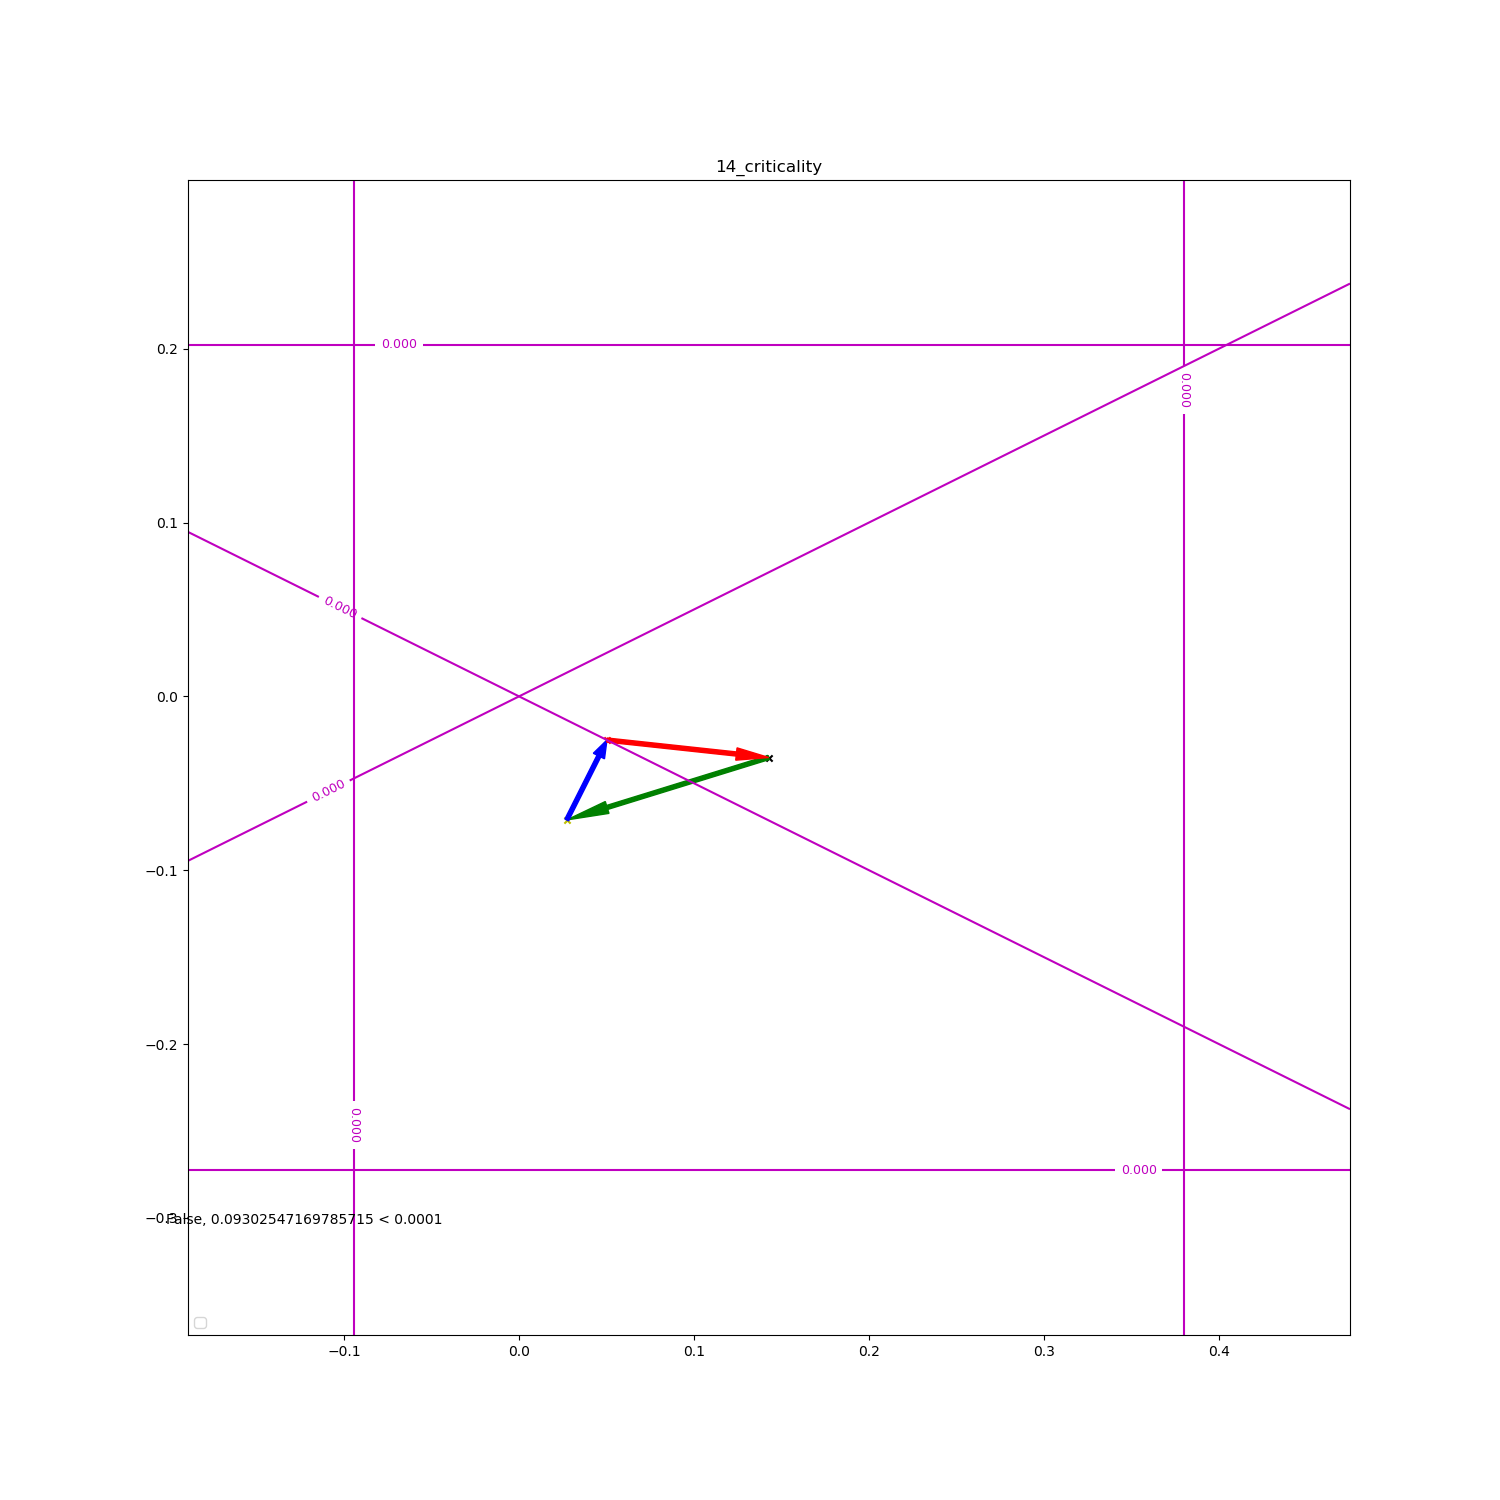
\includegraphics[width=200px]{images/algorithm_iterations/criticality_measure.png}
%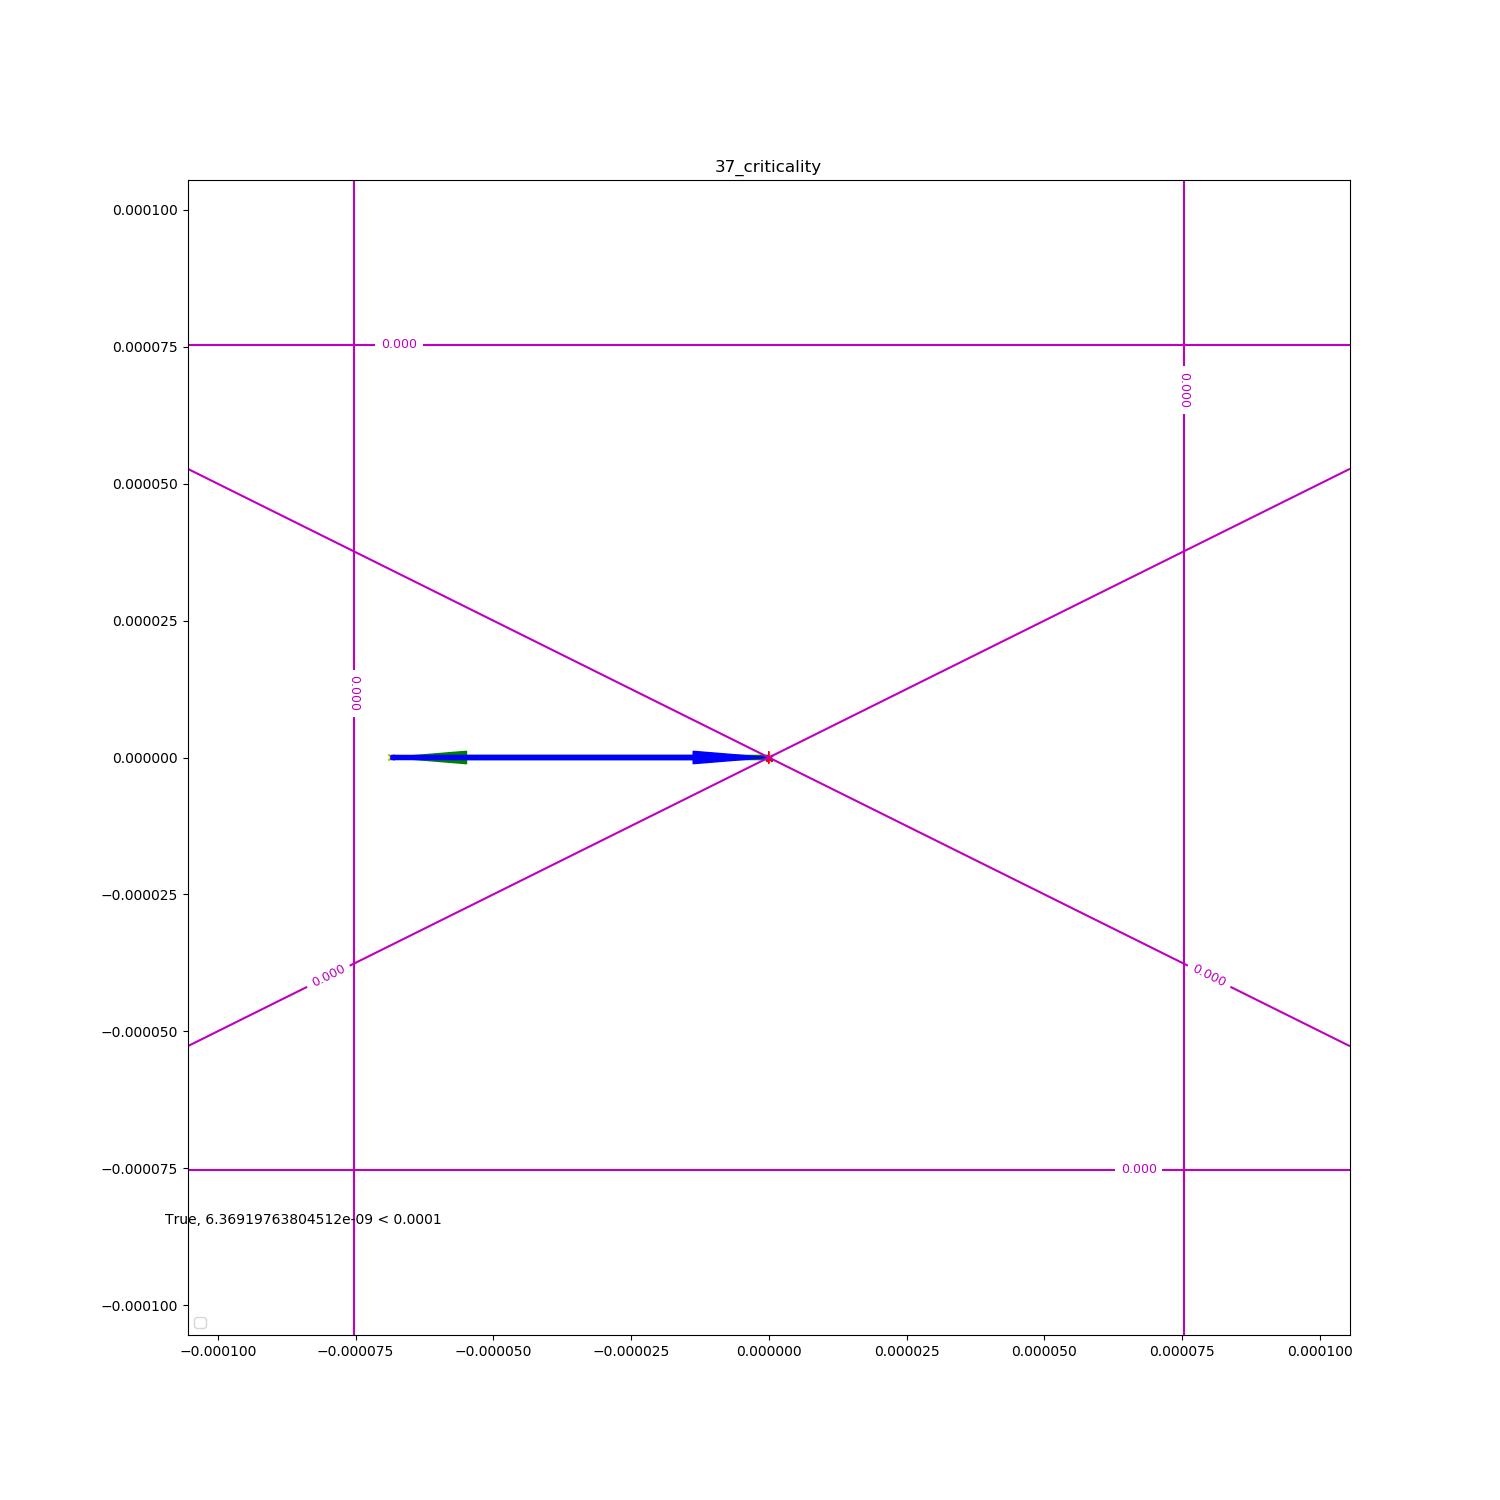
\includegraphics[width=200px]{images/algorithm_iterations/criticality_measure_critical.png}
%\end{center}

%That is, if $x^{\star}$ is a first order critical point satisfying

%\begin{align*}
%\nabla f(x^{\star}) + \sum_{i\in\mathcal I} \lambda_i \nabla c_i(x^{\star}) + \sum_{i\in \mathcal E} \mu_i \nabla c_i(x^{\star})  = 0 \\
%c(x^{\star})_i \mu_i = 0 & \quad \forall i\in\mathcal I \\
%c(x^{\star}) \le 0 & \quad \forall i\in\mathcal I\\
%c(x^{\star}) = 0 & \quad \forall i\in\mathcal E
%\end{align*}
%for some $\lambda_i \in \mathbb R$, and $\mu_i \ge 0$, then we need $\lim_{x\to x^{\star}} \chi(x) = 0$.

%This suggests the following definition:
%\begin{align}
%\label{critical}
%\chi & = & |\min_t \langle g_k + H_kn_k, t\rangle| \\
%& A_{\mathcal {E}}t &=& \; 0 \\
%& c_{\mathcal {I}} + A_{\mathcal {I}}t &\le& \; 0 \\
%& \| t \| &\le& \; 1
%\end{align}

%Notice that this must be computed after the normal step $n^k$ has been computed.

%\color{red}
\subsubsection{Sufficient reduction of model}

Within each iteration, it will be convenient to ensure sufficient reduction of the objective's model function.
We adopt the following condition:
\begin{equation}
\label{efficiency}
\modelk(\iteratek) - \modelk(\iteratek + \trialk) \ge \kappa_f \chi_k \min\{ \frac{\chi_k}{1+\|\nabla^2 \modelk(\iteratek)\|}, \Delta_k, 1 \}
\end{equation}
where $\kappa_f$ as a constant independent of $k$.
Our algorithm must ensure that this efficiency condition is satisfied.

This is widely used within trust region frameworks such as \cite{Conejo:2013:GCT:2620806.2621814} and \cite{Conn:2000:TM:357813}.
It can be shown that the \emph{generalized Cauchy point} satisifies this condition.

%The generalized Cauchy point extends the Cauchy point of following a line search along the gradient, but projects this line search onto the feasible region.
%To define the generalized Cauchy point, we first define 
%$P_X$ to be the projection operator on to the convex set $X$
%\[ p(t,x) = P_{\feasiblek}[x-t\nabla \modelk(x)] \]
%\[ \trialk(t) = p(t,\iteratek)-\iteratek \].

%If we parameterize this projected line search with a parameter $t$,
%the generalized Cauchy point is found at $t=t_j$ where the following conditions hold
%for some chosen fixed constants
%\begin{align}
%0 < \kappa_{ubs} < \kappa_{lbs} < 1, \quad \kappa_{frd} \in (0, 1), \quad \text{and} \quad\kappa_{epp} \in (0, \frac 1 2 ):
%\end{align}

%\begin{align}
%\label{too_big_1}
%\|\trialk(t_j)\|\le \Delta_k
%\end{align}
%\begin{center}and\end{center}
%\begin{align}
%\label{too_big_2}
%\modelk(p(t_j, \iteratek)) \le \modelk(\iteratek) + \kappa_{ubs}\langle \nabla\modelk(\iteratek), \trialk(t_j)\rangle
%\end{align}
%and at least one of
%\begin{align}
%\label{too_small_1}
%\|\trialk(t_j)\| \ge \kappa_{trd}\Delta_k
%\end{align}
%\begin{center}or\end{center}
% \begin{align}
% \label{too_small_2}
% \modelk(p(t_j, \iteratek)) \ge \modelk(\iteratek) + \kappa_{lbs}\langle \nabla\modelk(\iteratek), s_k(t_j)\rangle
% \end{align}
% \begin{center}or\end{center}
% \begin{align}
% \label{too_small_3}
% \|P_{\mathcal T(p(t_j, \iteratek))}[-\nabla\modelk(\iteratek)]\| \le \kappa_{epp} \frac{\langle \nabla\modelk(\iteratek), s_k(t_j) \rangle}{\Delta_k}
% \end{align}
% where $\mathcal T(x)$ is the tangent cone at $x$ with respect to $\feasiblek$.
% 
% 
% \color{red}
% It can be computed with the following algorithm:
% 
% \begin{algorithmic}
% \State $t_{\text{min}} \gets 0$
% \State $t_{\text{max}} \gets \infty$
% \State $t_{0} \gets \frac{\Delta_k}{\|g_k\|}$
% \State $j=0$
% \While{true}
%     \State{$p(t_j, x_k) \gets Proj_{X}(x_k-t_jg_k)$}
%     \State{$s_k(t_j) \gets p(t_j, x_k) - x_k$}
%     \State Evaluate $m_k(p(t_j, x_k))$
%     \If{\ref{too_big_1} or \ref{too_big_2} is violated}
%         \State{$t_{\text{max}} \gets t_j$}
%     \ElsIf{\ref{too_small_1} and \ref{too_small_2} and \ref{too_small_3} are violated}
%         \State{$t_{\text{min}} \gets t_j$}
%     \Else
%         \State \textbf{return}  $p(t_j, x_k)$
%     \EndIf
%     \If{$t_{\text{max}} = \infty$}
%         \State{$t_{j+1} \gets 2t_{j}$}
%     \Else
%         \State{$t_{j+1} \gets \frac 1 2 (t_{\text{min}} + t_{\text{max}})$}
%     \EndIf
%     \State{$j \gets j+1$}
% \EndWhile
% \end{algorithmic}
% 
% \color{black}

\subsubsection{Trust regions}
Our algorithm maintains two trust regions.
The outer trust region is an $L_1$ ball of radius $\Delta_k$ defined by
\begin{equation}
\label{trust_region}
\outertrk = B_{\infty}(\iteratek,\Delta_k) = \{x\in \mathbb R^n | \; {\iteratek}_i - \Delta_k \le x_i \le {\iteratek}_i + \Delta_k \quad \forall 1\le i \le n\}.
\end{equation}

Within iteration $k$, the first step is to construct the inner trust region $\innertrk$ which can take many different forms.
Note that regardless of the choice of inner trust region, we always seek
$\innertrk \subseteq \outertrk $, and $\iteratek \in \innertrk$.


We have considered two general strategies to solve this problem.

\begin{itemize}
\item Force $\label{bluepill} \innertrk \subseteq \outertrk \cap \feasiblek$ to have an ellipsoidal shape.
\item Take $\label{redpill} \innertrk = \outertrk \cap \feasiblek$ and ensure model accuracy over a polyhedral domain.
\end{itemize}

The advantage of the first approach is that we can reuse classical methods for ensuring good geometry.
We can choose $\innertrk$ to be ellipsoidal and use efficient algorithms within \cite{DUMMY:intro_book} to satisfy \ref{accuracy}.
However, we must be careful to choose $\innertrk$ to allow sufficient reduction when we solve the trust region subproblem using the inner trust region.


We have two choices for this trust region subproblem:
\begin{align}
\trialk = \min_{\trialk \in \innertrk \subset \feasiblek} \modelk(\iteratek + \trialk) \\
\trialk = \min_{\trialk \in \outertrk \cap \feasiblek} \modelk(\iteratek + \trialk)
\end{align}

In either case, work to find a point satisfisfying \ref{efficiency} and 
\begin{equation}
\label{accuracy}
\|\nabla \modelk(\iteratek) - \nabla f(\iteratek) \| \le \kappa_g \Delta_k
\end{equation}
 for some fixed constant $\kappa_g$ is a fixed constant independent of $k$.

 

To complete the second approach $\innertrk = \outertrk \cap \feasiblek$, we need some redefinition of poisedness for polyhedral shapes.
However, since the trust region is larger, it is easier to find sufficient reduction.
This strategy also has the drawback that it will force sample points close to the boundary of the feasible region.
If we only model the boundary, this may mean more infeasible evaluation attempts.

The classical methods for ensuring good geometry require an optimization call to the model functions over the entire trust region.
This is no longer possible in the second strategy.
However, the bounds produced over the entire trust region may also be stronger than required as the models will only be used on the feasible region.
This may mean the geometric requirements can be reduced.
Looking again at the ill-poised set, the set of nearly colinear sample points actually does appear to be accurate over a smaller trust region:


\begin{figure}[h]
    \centering
    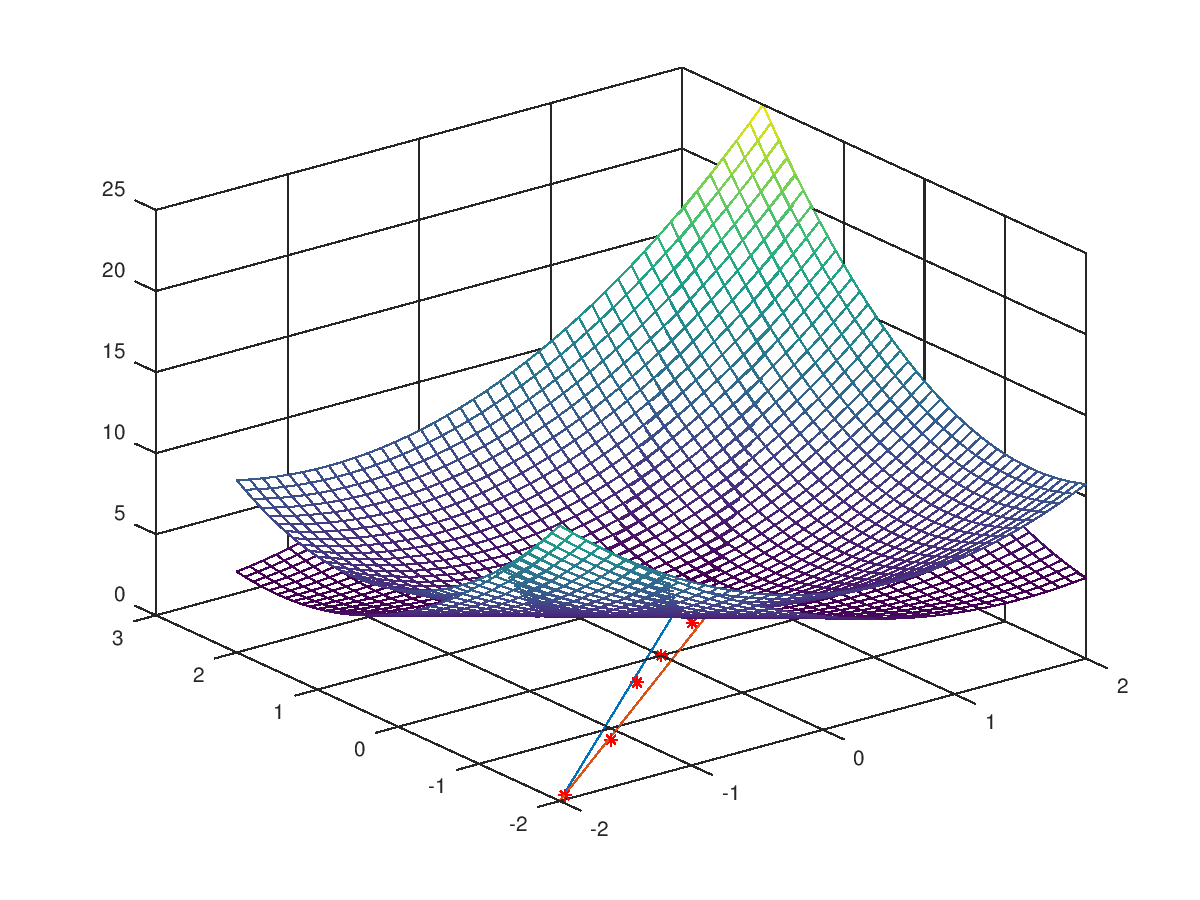
\includegraphics[width=200px]{images/poised_bad_but_good.png}
    \caption{Accurate model over thin trust region from illpoised set}
    \label{aoip}
\end{figure}


Within our algorithm, when $ \outertrk \subseteq \feasiblek$ we can default the trust region to the ellipsoid sphere.
This saves the computation of $\innertrk$ when it is not needed, as there are no nearby constraints.

\subsection{Algorithm Template}

Although some details depend on the particular choice of $\innertrk$, we follow an algorithm template described in \cite{doi:10.1080/10556788.2015.1026968}.

% HOW ABOUT JUST MAKE $\eta > 0$?

\begin{algorithmic}

\State $x^{(0)} \in \domain$
\State $\alpha > 0, 0 < \Delta_0 < \Delta_{\text{max}} < \frac 1 2 diam(\domain), 0 < \gamma_{0} < 1 \le \gamma_{1}, \eta_1 \in (0,1), 0 \le \eta < \eta_1 \le \eta_2$
\State $k \gets 0$
\Loop
    \State $\innertrk\gets $ \Call{ConstructTrustRegion}{$\Delta_k, x^{(k)}$}
    \State Ensure that the sample points are poised with respect to $\innertrk$ for \ref{accuracy}
    \State Construct $\modelk$ as in \ref{reg}
    \State Compute $\chi_k$ as in \ref{critical}
    \If{$\Delta_k > \alpha \chi_k$}
        \State $\Delta_{k+1} \gets \gamma_1 \Delta_{k}, x^{(k+1)} \gets \iteratek$
    \Else
        \State $\trialk = \min_{s \in \outertrk \cap \domain} \modelk(\iteratek + \trialk)$
        \State Evaluate $f(\iteratek + \trialk)$ and construct $\rho_k$ as in \ref{rho}
        \If{$\rho_k > \eta$}
            \State $ \iteratekpone \gets \iteratek + \trialk$
        \Else
            \State $\iteratekpone \gets \iteratek $
        \EndIf
        \If{$\rho_k < \eta_1$}
            \State $\Delta_{k+1} \gets \gamma_1\Delta_k$
        \Else
            \If{$\rho_k > \eta_2 \wedge \|\trialk\| = \Delta_k$}
                \State $\Delta_{k+1} \gets \gamma_1\Delta_k$
            \Else
                \State $\Delta_{k+1} \gets \Delta_{k}$
            \EndIf
        \EndIf
    \EndIf
    \State $k \gets k+1$
\EndLoop
\end{algorithmic}

Much of the work is defered to the ConstructTrustRegion subroutine.
We will describe several different approaches we have taken for this subroutine.
For convergence analysis, \ref{accuracy} must be satisfied by the trust region choice in this method.
Not all searches for an inner trust region must guarantee this: the algorithm is allowed to try a bounded number of trust regions as long as one is gauranteed to satisfy these conditions.
In some cases, multiple inner trust regions may be considered before returning the best trust region found.
An efficient algorithm may first heuristically search for a good trust region if the garaunteed method is expensive.
This may not involve constructing a model or function evaluations.





%
%The following example shows a prototypical subroutine implementation:
%
%\begin{algorithmic}
%\Procedure{ConstructTrustRegion}{}
%    \State $T_{\text{in}} \gets \empty$
%    \ForAll{$T_{\text{trial}$}
%        \State check heuristic
%    \EndFor
%\EndProcedure
%\end{algorithmic}



\noindent\makebox[\linewidth]{\rule{\paperwidth}{0.4pt}}

MORE SIMILAR TO WHAT I HAVE CODED:

REPLACE $\gamma$ with $\eta$.
\begin{enumerate}
    \item Initialize $k=0$, $0<\gamma_1<\gamma_2<1$,$\tau_{\chi}>0$,$\tau_{\Delta}>0$, $\Delta_0 > 0$, $x_0$ a feasible starting point, $0<\omega_{\text{dec}} < 1 \le \omega_{\text{inc}}$, $\gamma_{\Delta}$
    \item Compute the inner trust region.
    \begin{itemize}
        \item This may mean maximizing an ellipse as in \ref{ellipse_optimization}
    \end{itemize}
	\item Ensure poisedness, and create the model functions ${m_f}_k(x)$, ${c_i}_k(x), i \in \mathcal I \cup \mathcal E$ as described in \ref{reg}
	\item Compute criticality measure $\chi_k = \chi(x_k)$ as described in \ref{critical}
    \begin{itemize}
        \item If $\chi_k < \tau_{\chi}$ and $\Delta_k \le \tau_{\Delta}$, return as converged
        \item If $\chi_k < \tau_{\chi}$ and $\Delta_k > \tau_{\Delta}$, then $\Delta_{k+1} \leftarrow \omega_{\text{dec}} \Delta_k$, $k \leftarrow k + 1$
    \end{itemize}
	
	\item Solve the Trust region subproblem: $s^{(k)} = \argmin_{s\in B(x^{(k)};\Delta_k)} m_k(x^{(k)} + s)$
	
	\item Test for improvement
	\begin{itemize}
		\item Compute $\rho_k$ using \ref{rho}
    \item Update the outer trust region $\Delta_k$
		\item If $\rho < \gamma_1$, then $x^{(k+1)}=x^{(k)}$ (reject) $\Delta_{k+1} \leftarrow \omega_{\text{dec}} \Delta_k$
		\item If $\gamma_1 \le \rho \le \gamma_2$, then $x^{(k+1)}=x^{(k)}+s^{(k)}$ (accept) and $\Delta_{k+1} \leftarrow \omega_{\text{dec}} \Delta_k$
		\item If $\rho > \gamma_2$, then $x^{(k+1)}=x^{(k)}+s^{(k)}$ (accept)
		\begin{itemize}
            \item If $\|x^{(k)} - s^{(k)} \| < \gamma_{\Delta} \Delta_k$ then $\Delta_{k+1} \leftarrow \omega_{\text{dec}} \Delta_k$
            \item else $\Delta_{k+1} \leftarrow \omega_{\text{inc}} \Delta_k$
		\end{itemize}
	\end{itemize}
    $k \leftarrow k + 1$
	\item Go to step 2
\end{enumerate}
\noindent\makebox[\linewidth]{\rule{\paperwidth}{0.4pt}}

\subsection{First Approach: Bumping $\xi$}
One simple approach to handle partially-quantifiable constraints is to simply avoid letting points fall outside the feasible region.
Within the model improvement algorithm to select new points, we constrain the new points to also lie within the current model of the trust region.

The problem lies in finding suffiently poised sample points.
The classical model algorithm uses a parameter $\xi$ as a lower bound of the pivot values of the Vandermode matrix.
When requiring points to live within the trust region intersect the feasible region, it can happen that even after replacing a point, we still have not satisfied this bound.
In figure \ref{lspc}, the sample points are not be poised for some values $\xi$, however no better points exist within the feasible region intersect the trust region.

\begin{figure}[h]
    \centering
    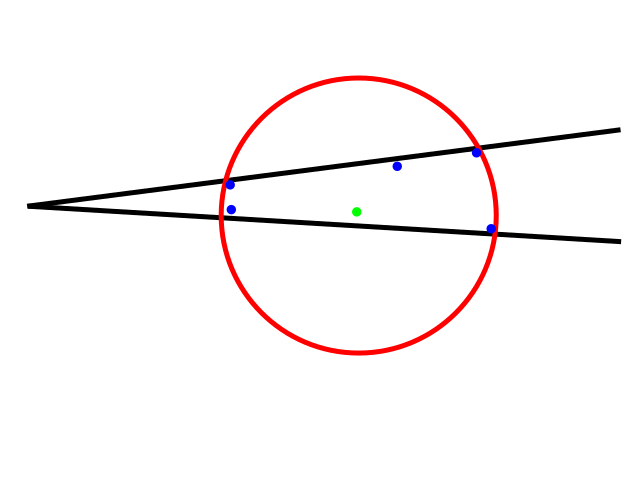
\includegraphics[scale=0.4]{images/bad_lambda.png}
    \caption{Limited sample point choice}
    \label{lspc}
\end{figure}

As the number of dimensions grows the ratio of volume of the trust region intersect the feasible region to the feasible region can become smaller.

One way to handle this is to simply allow $\xi$ to decrease. (Possibly, until a threshold is reached for maintaining a fixed $\Lambda$.)
If the new point does not improve the geometry of the set significantly, then there is no other point that would do better.
In this case, we cannot do better and simply proceed with our current point.



\subsubsection{Requiring sufficient model improvement}

The new modified improvement algorithm is as follows:

\begin{algorithmic}[1]
\State $0 < \xi_{\text{min}} < \xi_{\text{desired}}$, $0 <\delta_{\text{improv}} < 1$
\State initialize shifted set $y$, vandermode matrix $V_{i,j} = \phi_j(y^i)$ constants
\State $\xi_{\text{cur}} \gets \xi_{\text{desired}}$
\For{$i = 1 \ldots p$}
    \State Swap row $i$ with row $i_{\max} = \arg \max_{j\ge i} V_{j,i} $
    \If {$|V_{i,i}| < \xi_{\text{cur}}$}
        \State $y' = \arg\max_{t \in T_K \cap X} |\phi_i(t)|$
        \State $v = |\phi_i(y')|$
        \If {$\label{impossibly_poised} v < \xi_{\text{min}}$}
            \State $\mathbf {fail}$
        \EndIf
        \If {$\xi_{\text{cur}} - v > \delta_{\text{improv}} \xi_{\text{cur}}$}
            \State Replace $V_i$ with $y'$
        \EndIf
    \EndIf
    \State $V_i \gets \frac{V_i}{V_{i,i}} $
    \For{$j=i \ldots p$}
        \State $V_{,j} \gets V_{, j} - V_{i,j} V_{, i}$
    \EndFor
\EndFor
\end{algorithmic}

As is usual, we may also wish to remove points larger than a certain radius from the current model center.
The construct model routine for this approach follows the protype with $T_{in} = X \cap  T_k$.
If a lower bound on the maximum value of each polynomial is known ahead of time, then the check on \ref{impossibly_poised} is not needed.

Another interesting approach we have not investigated is to decrease the size of the sample set when a new point cannot be computed.


The analysis for this approach may be more difficult.




\subsection{Second Approach: Feasible trust regions}

If we adopt the second approach to maintain a feasible inner trust region with a ``nice" shape, we will be ensured of a weaker version of \ref{accuracy}.
Namely, we will know that 
\[\
    \|\modelk(x) - \nabla f(x) \| \le \kappa_g \Delta_{\text{inner}} \quad \forall x \in T_{\text{in}}.
\]
If bounds can be shown relating the model error of the inner trust region to the outer trust region, then we will satisfy \ref{accuracy}.
%In this case, classical methods ensure that $\|\nabla f(x^{(k)}) - \nabla m_f(x^{(k)})\| < \Delta_{inner} \le \Delta_k$.

\subsubsection{Circular trust region}
The simplest approach to maintaining a feasible trust region is to set the inner trust region radius sufficiently small.
Within the construct inner trust region subroutine, this method sets the trust region radius to the minimum distance to the any constraint:
$\outertrk = B_2(\iteratek, \min\{\Delta_k, \min_{i}\frac{|A_i\iteratek - b_i|}{\|A_i\|} \})$.

In practice, this does not work well as the radius can become too small to allow any progress.

\begin{figure}[h]
    \centering
    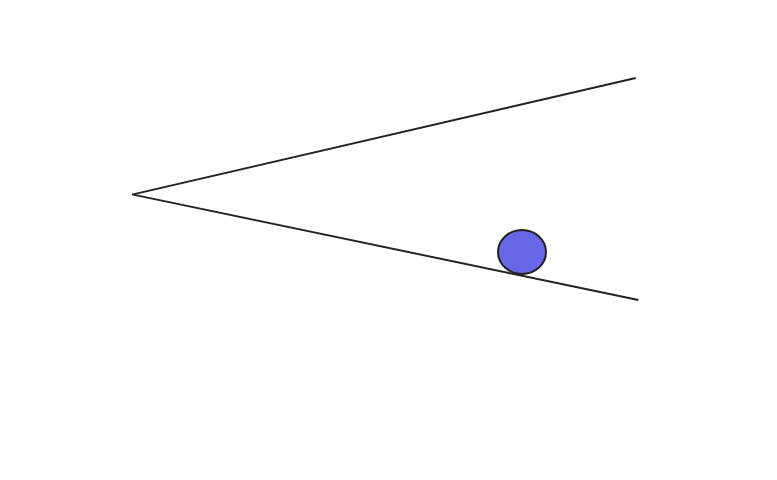
\includegraphics[width=200px]{images/BAD_CIRCLE.png}
    \caption{A bad trust region}
\end{figure}


    
\subsubsection{Ellipsoids}

In order to address this issue we also considered using ellipsoidal trust regions.
Whereas the circle does not allow improvement when the current iterate lies along a constraint, an ellipse elongates along this constraint.
In figure \ref{ellipse_adv}, we have this type of iterate, but by using an ellipse we are still able to search towards the vertex of the feasible region.
\begin{figure}[h]
    \centering
    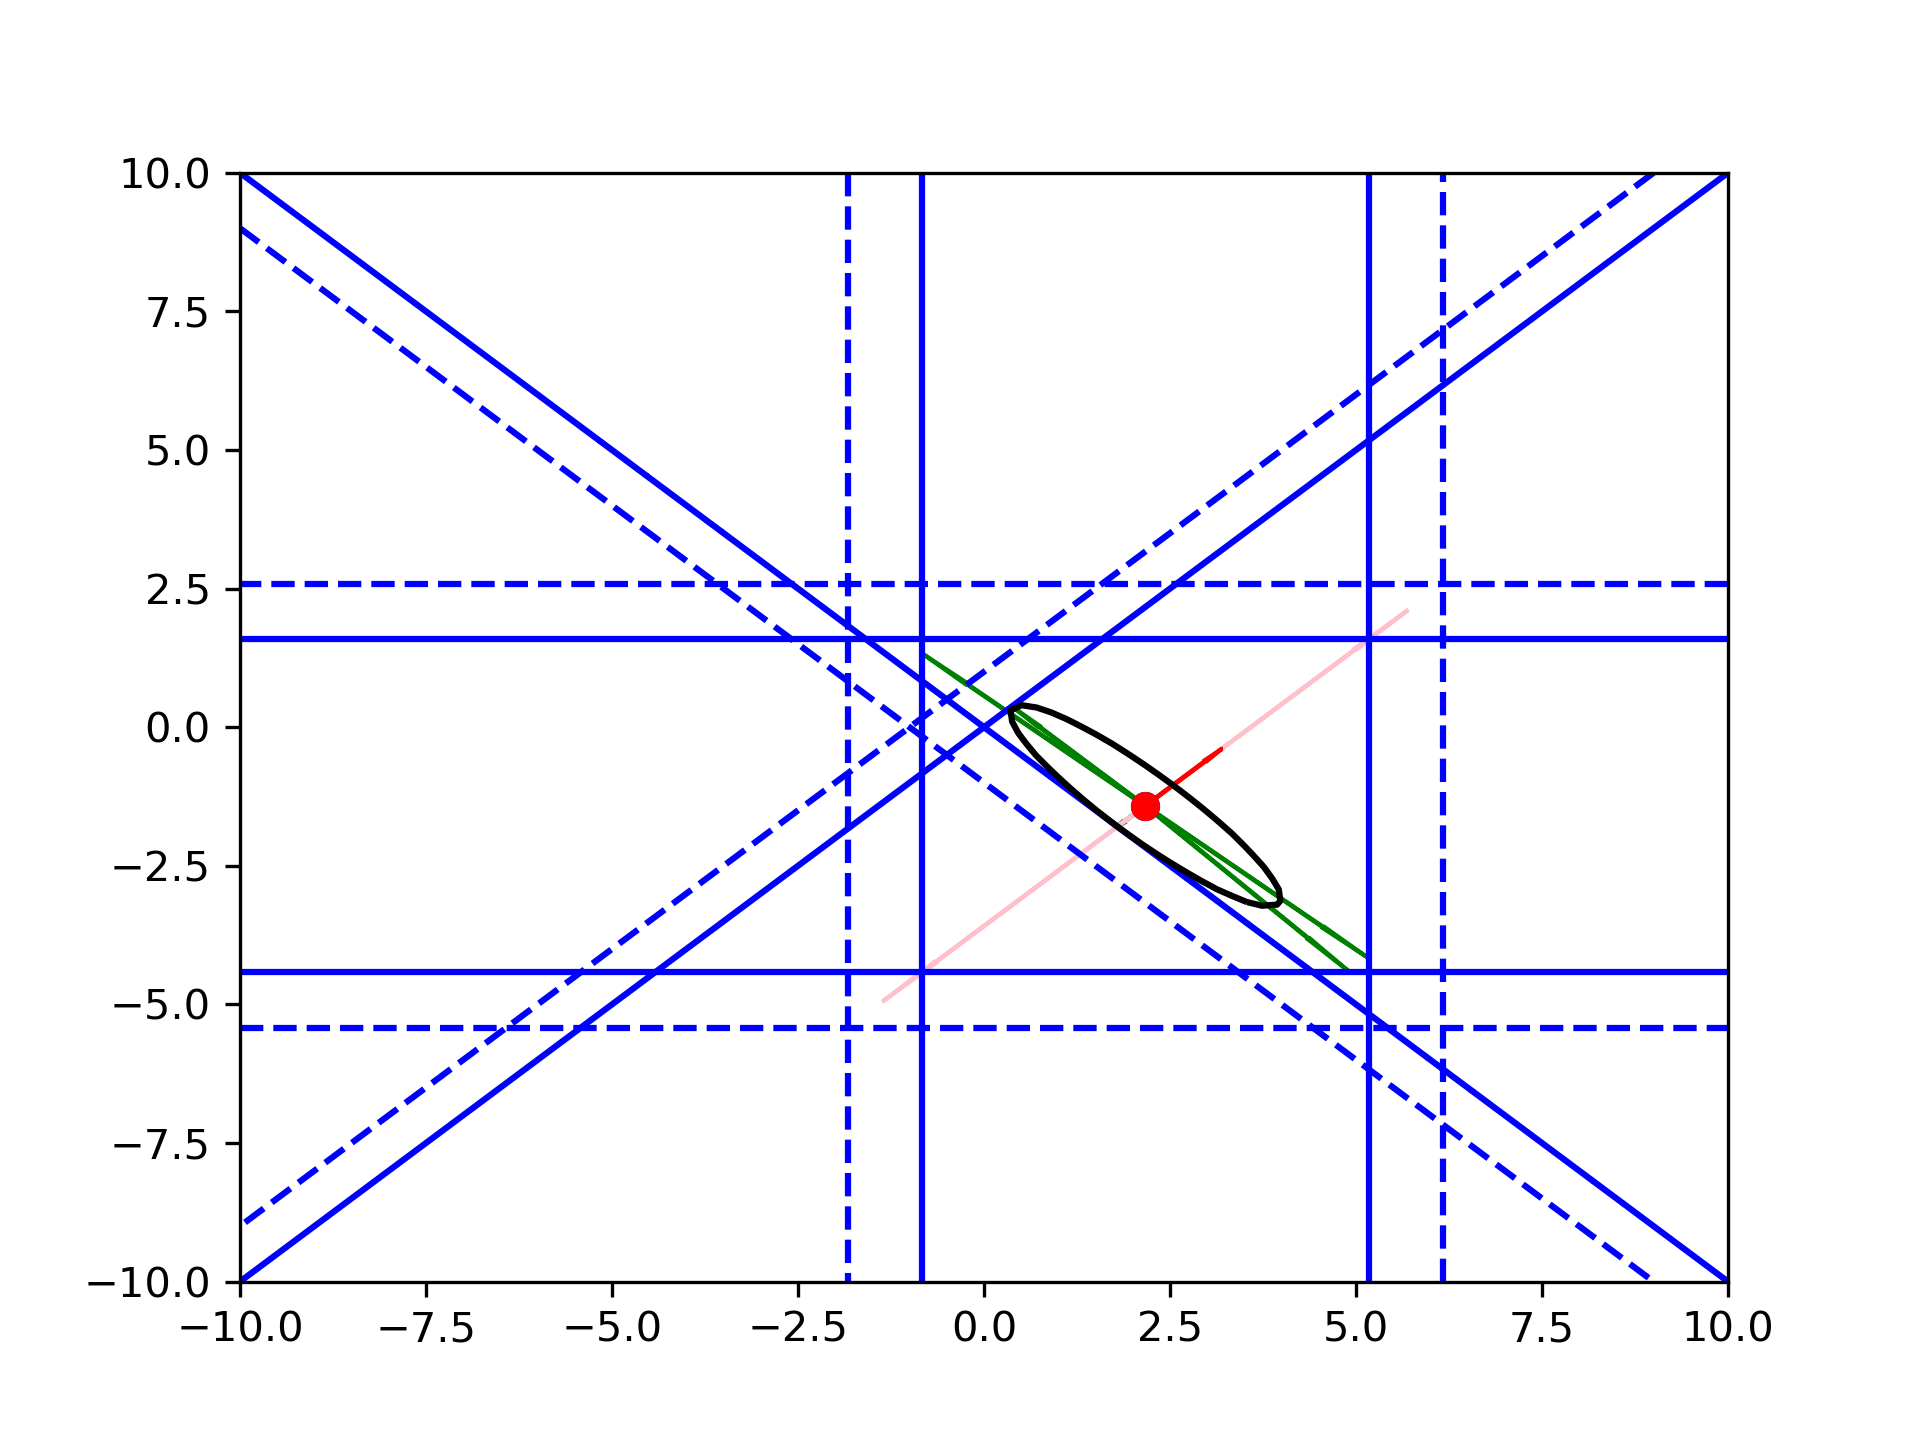
\includegraphics[scale=0.4]{images/advantage_of_ellipse_2.png}
    \caption{a nice plot}
    \label{ellipse_adv}
\end{figure}


More specifically, at iteration $k$, we choose a scaling factor $\pi^k$ and solve for an ellipse center $\mu^k$ and positive definite matrix $Q^k$ to define an ellipse
$ \ellipsek = \{x \in \mathbb R^n \| \pi^k - \frac 1 2 (x - \mu^{k})^TQ^{k}(x - \mu^{k}) \ge 0 \}$.
We then map this back to the origin with the affine transformation $T^k : \mathbb R^n \to R$ $T^k(x) = \frac {\sqrt{2}}{\pi^k} L^k(x-\mu^k)$ where $L = cholesky(Q)$.
This allows us to construct a lambda poised set within narrow trust regions.
The simplest approach is to not change the center of the ellipse, but instead let $\mu^k = x^k$.

There are a number of issues to be solved to define this ellipse:
\begin{itemize}
\item How do we ensure that $x^{(k)} \in E^k$?
\item How do we choose the center of the ellipse $\mu^k$?
\item Is $ \ellipsek \subset T_k \cap \domain$?
\end{itemize}

We have implemented a few ways of ensuring the current iterate is within the trust region, $x^{(k)} \in E^k$.
If we do not include the current iterate within the interior of $T_{k}$, we likely lose sufficient reduction.
This can be done by either expanding the radius of the ellipse, or by including the original point as a constraint for the ellipse problem.

%IMAGES GO HERE

In order to include the original point as a constraint, we add a constraint to the definition of the ellipse of the following form:
$$ \pi^k - \frac 1 2 (x^k - \mu^{k})^TQ^{k}(x^k - \mu^{k}) \ge 0. $$
Constraints of this nature make the optimization problem of finding the ellipse much more expensive.
This is because the optimization problem we construct to find $Q^k$ solves for ${Q^k}^{-1}$, so that adding this constraint is a constraint on the inverse of $Q^k$.


%\begin{center}
%\begin{align}
%\label{problem}
%\min_x & \quad m_f(x) \\
%  m_{c_i}(x) \le 0   & \quad \forall i \in \mathcal {I} \nonumber \\
%  m_{c_i}(x)  = 0    & \quad \forall i \in \mathcal {E} \nonumber \\
%  \bar{x}^T Q^k \bar{x} \le s^k
%\end{align}
%\end{center}


The alternative is to scale $Q$ by a constant.
To do this, we use the scaling factor $\pi^k$ by defining it to be

$$\pi^k = \max \{1, \frac 1 {2} (x^{k} - \mu^{k})^T Q^k (x^{k} - \mu^{k})^T \}$$

and let the ellipse be:
$$E_k = \{x \in \mathbb | 1 - \frac 1 {2\pi^k} (x - \mu^{k})^T Q (x - \mu^{k}) \ge 0\} $$
However, this means that we do not ensure $E_k \subset F_k$ so that the trust region subproblem must contain constraints for both the ellipse and the feasible region: $T_{in} = E_K \cap \domain$.

The are several concerns to be considered while defining the ellipse.
The major concern is that we can accidently define $\ellipsek$ in such a way that it limits travel along a decent direction.
We also want consecutive ellipse to share volume, in order to avoid evaluating as many points as possible.
(So far, we have been re-evaluating the set of trial points each iteration.)


Also, unless we include points outside the ellipse, we cannot find a second order solution because the ellipse can only be tangent to the constraint.
In figure \ref{fbns}, the red line represents a path in the feasible region that is always decreasing.
However, if the trust regions decrease without intersecting this path, the algorithm will not be aware of this descent direction.
However, scaling the trust region to the outer green radius may allow the algorithm to ensure global convergence to second order critical points.

\begin{figure}[h]
    \centering
    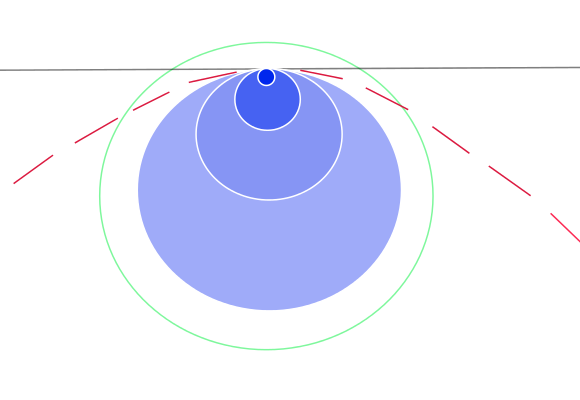
\includegraphics[width=200px]{images/second_order_critical_point.png}
    \label{fbns}
\end{figure}



Finally, we have the problem of computing the ellipse once given a suitable definition.
In order to provide the most search space available within the trust region subproblem, we maximize the volume of the ellipse.

\subsubsection{Finding the maximal $E_k$ given $\mu^k$}

\label{ellipse_optimization}

Here, we first solve the problem of finding the maximum-volumne ellipse given the center, and then perform a search over different centers of the ellipse.
Because of this, we will first show how to find an ellipse with maximum volume given a fixed center.
We adopt a method similar to \cite{Khachiyan1993}.
For now, we also let $\pi^k = 1$.

Given a polyhedron $P$ defined by an $m \times n$ matrix $A$,
\[
P = \{ x \; | \;  Ax \le b \},
\]
we wish to find the maximum-volume ellipse $E \subset P$ centered at a point $\mu^{k}$ within this polyhedron.

We can shift the polyhedron by letting $\bar{b} = b - A\mu^{k}$ and letting $d \to x - \mu^{k}$ so that the polyhedron becomes
\[
P = \{ \mu^k + d \; | \;  Ad \le \bar{b} \}
\]
The ellipse can then be centered at zero, and defined by a symmetric positive definite matrix $Q \succ 0$:
\[
E = \{ d \; | \; \frac 1 2 d^T Q d \le 1 \}.
\]
We define the auxiliary function 
\[
f(d) = \frac 1 2 d^T Q d
\]
so that this becomes
\[
E = \{ d \; | \; f(d) \le 1 \}.
\]

At the locations where the ellipse intersects the polyhedra with minimum value of $f$, the gradients of $f$ must be orthogonal to the faces.
Each face is defined by $A_i x \le \bar{b}_i$ for some $i$ where $A_i$ is the $i$th row of $A$ for $1\le i \le m$.
This implies that if $d^{(i)}$ is such a point along a face, then

% SOME OF THESE LINES CAN BE REMOVED


\[
\nabla f(d^{(i)}) = \lambda_i A_i \quad \forall 1\le i\le m
\]
for some $\lambda_i \ge 0$.
This means
\[
Q d^{(i)} = \lambda_i A_i \quad \forall 1\le i\le m
\]
\[
d^{(i)} = \lambda_i Q^{-1}A_i \quad \forall 1\le i\le m
\]
We also know that 
\[
A_i^T d^{(i)} = \bar{b} \quad \forall 1\le i\le m
\]
\[
A_i^T \lambda_i Q^{-1}A_i = \bar{b} \quad \forall 1\le i\le m
\]
\[
\lambda_i = \frac {\bar{b}}{A_i^T  Q^{-1}A_i} \quad \forall 1\le i\le m
\]
so that 
\[
d^{(i)} = \lambda_i Q^{-1}A_i \forall 1\le i\le m
\]
\[
d^{(i)} = \frac {\bar{b}}{A_i^T  Q^{-1}A_i}  Q^{-1}A_i \quad \forall 1\le i\le m.
\]

Finally, we need that for each $i$, $f(d^{(i)}) \le 1$:
\[
\frac 1 2 (d^{(i)})^{T} Q d^{(i)} \le 1
\]
\[
\frac 1 2 (\frac {\bar{b}}{A_i^T  Q^{-1}A_i}  Q^{-1}A_i)^{T} Q \frac {\bar{b}}{A_i^T  Q^{-1}A_i}  Q^{-1}A_i \le 1
\]
\[
\frac 1 2 \frac {1}{A_i^T  Q^{-1}A_i}  \bar{b}^T A_i^T Q^{-1} Q \frac {\bar{b}}{A_i^T  Q^{-1}A_i}  Q^{-1}A_i \le 1
\]
\[
\frac 1 2 \frac {1}{A_i^T  Q^{-1}A_i}  \bar{b}^T \frac {\bar{b}}{A_i^T  Q^{-1}A_i}  A_i^T Q^{-1}A_i \le 1
\]
\[
\frac 1 2 \bar{b}^T \frac {\bar{b}}{A_i^T  Q^{-1}A_i} \le 1
\]
\[
\frac 1 2 \bar{b}^T \bar{b}\le A_i^T  Q^{-1}A_i
\]
\[
A_i^T  Q^{-1}A_i \ge \frac 1 2 \bar{b}^T \bar{b}
\]

Thus, the maximal ellipse is defined by

\[
\sup_{Q \succeq 0} \det(Q^{-1})
\]
\[
s.t. \quad A_i^T Q^{-1} A_i \ge \frac 1 2 \bar{b}^T\bar{b}
\]


This problem includes a maximization of a determinant.
In order to ensure that the trust region goes to zero, we must also ensure that the maximum eigenvalue of the matrix is bounded.
Thus, for some bound $M^k$ we define $Q^k$ as

\begin{center}
\begin{align}
\label{ellipse_1}
Q^k = V(\mu^k) = \sup_{Q \succ 0} & \det(Q^{-1}) & \\
  & {A^k}_i^T Q^{-1} {A^k}_i \ge \frac 1 2 (b^k - A^k\mu^{k})^T(b^k - A^k \mu^{k}) & \\
  & eig(Q)_i \le M^k & \forall i \in \mathcal I \cup \mathcal E \\
  & \pi^k - \frac 1 2 (x^k - \mu^{k})^TQ^{k}(x^k - \mu^{k}) \ge 0
\end{align}
\end{center}

if we wish to include the original point explicitly.
This gives rise to the trust region sub problem of

$$\innertrk = \{x \in \mathbb | 1 - \frac 1 {2s^k} (x - \mu^{k})^T Q (x - \mu^{k}) \ge 0\} $$
$$\trialk = \max \{1, \frac 1 {2} (\iteratek - \mu^{k})^T Q^k (\iteratek - \mu^{k})^T \}$$


\subsection{Searches for the center}

We may wish to shift $\mu^k$, allowing for more general ellipses.
In this case, our \emph{ConstructTrustRegion} subroutine searches over multiple centers of the ellipse, however it may not need to construct the model functions for each until it has found a desirable ellipsoid.

Given a huristic $H : \innertrk \to \Theta$, where $\Theta$ is a set of comparable elements, the \emph{ConstructTrustRegion} routine follows the following template:

\begin{algorithmic}
\Procedure{ConstructTrustRegion}{}
    \State $T_{\text{best}} = \emptyset$
    \State $\theta_{\text{best}} = H(T_{\text{best}})$
    \ForAll{$\mu \in$ search path}
        \State $T_{\text{trial}} \gets \arg\max_{E_k \text{centered at} \mu} \text{Vol}(E_k)$
        \State $\theta_{\text{trial}} = H(T_{\text{trial}})$
        \If{$\theta_{\text{trial}} > \theta_{\text{best}}$}
            \State $T_{\text{best}} = T_{\text{trial}}$
            \State $\theta_{\text{best}} = \theta_{\text{trial}}$
        \EndIf{}
    \EndFor
\EndProcedure
\end{algorithmic}

In most cases, we have simply used the heurstic $H(E_k) \to \text{Vol}(E_k)$.

\subsubsection{Search everything}

One approach is to search all possible centers within the feasible region intersect the trust region:
$ \feasiblek \cap \outertrk$.
That is, we add the constraints directly to the trust region subproblem by modifying \ref{ellipse_1}:
$$\mu^k = \sup_{\mu \in \feasiblek \cap \outertrk} V(\mu)$$
The search path within the \emph{ConstructTrustRegion} is allowed to go anywhere within $ \feasiblek \cap \outertrk$.
This has the advantage that it captures much of the feasible region.
However, one problem with this search is that it can force the trust region away from the desired direction.
Notice that in figure \ref{ellipse_runs_away}, although the ellipse found has larger volume than before being shifted, this volume contains points further from corner containing the minimizer.

\begin{figure}[h]
    \centering
    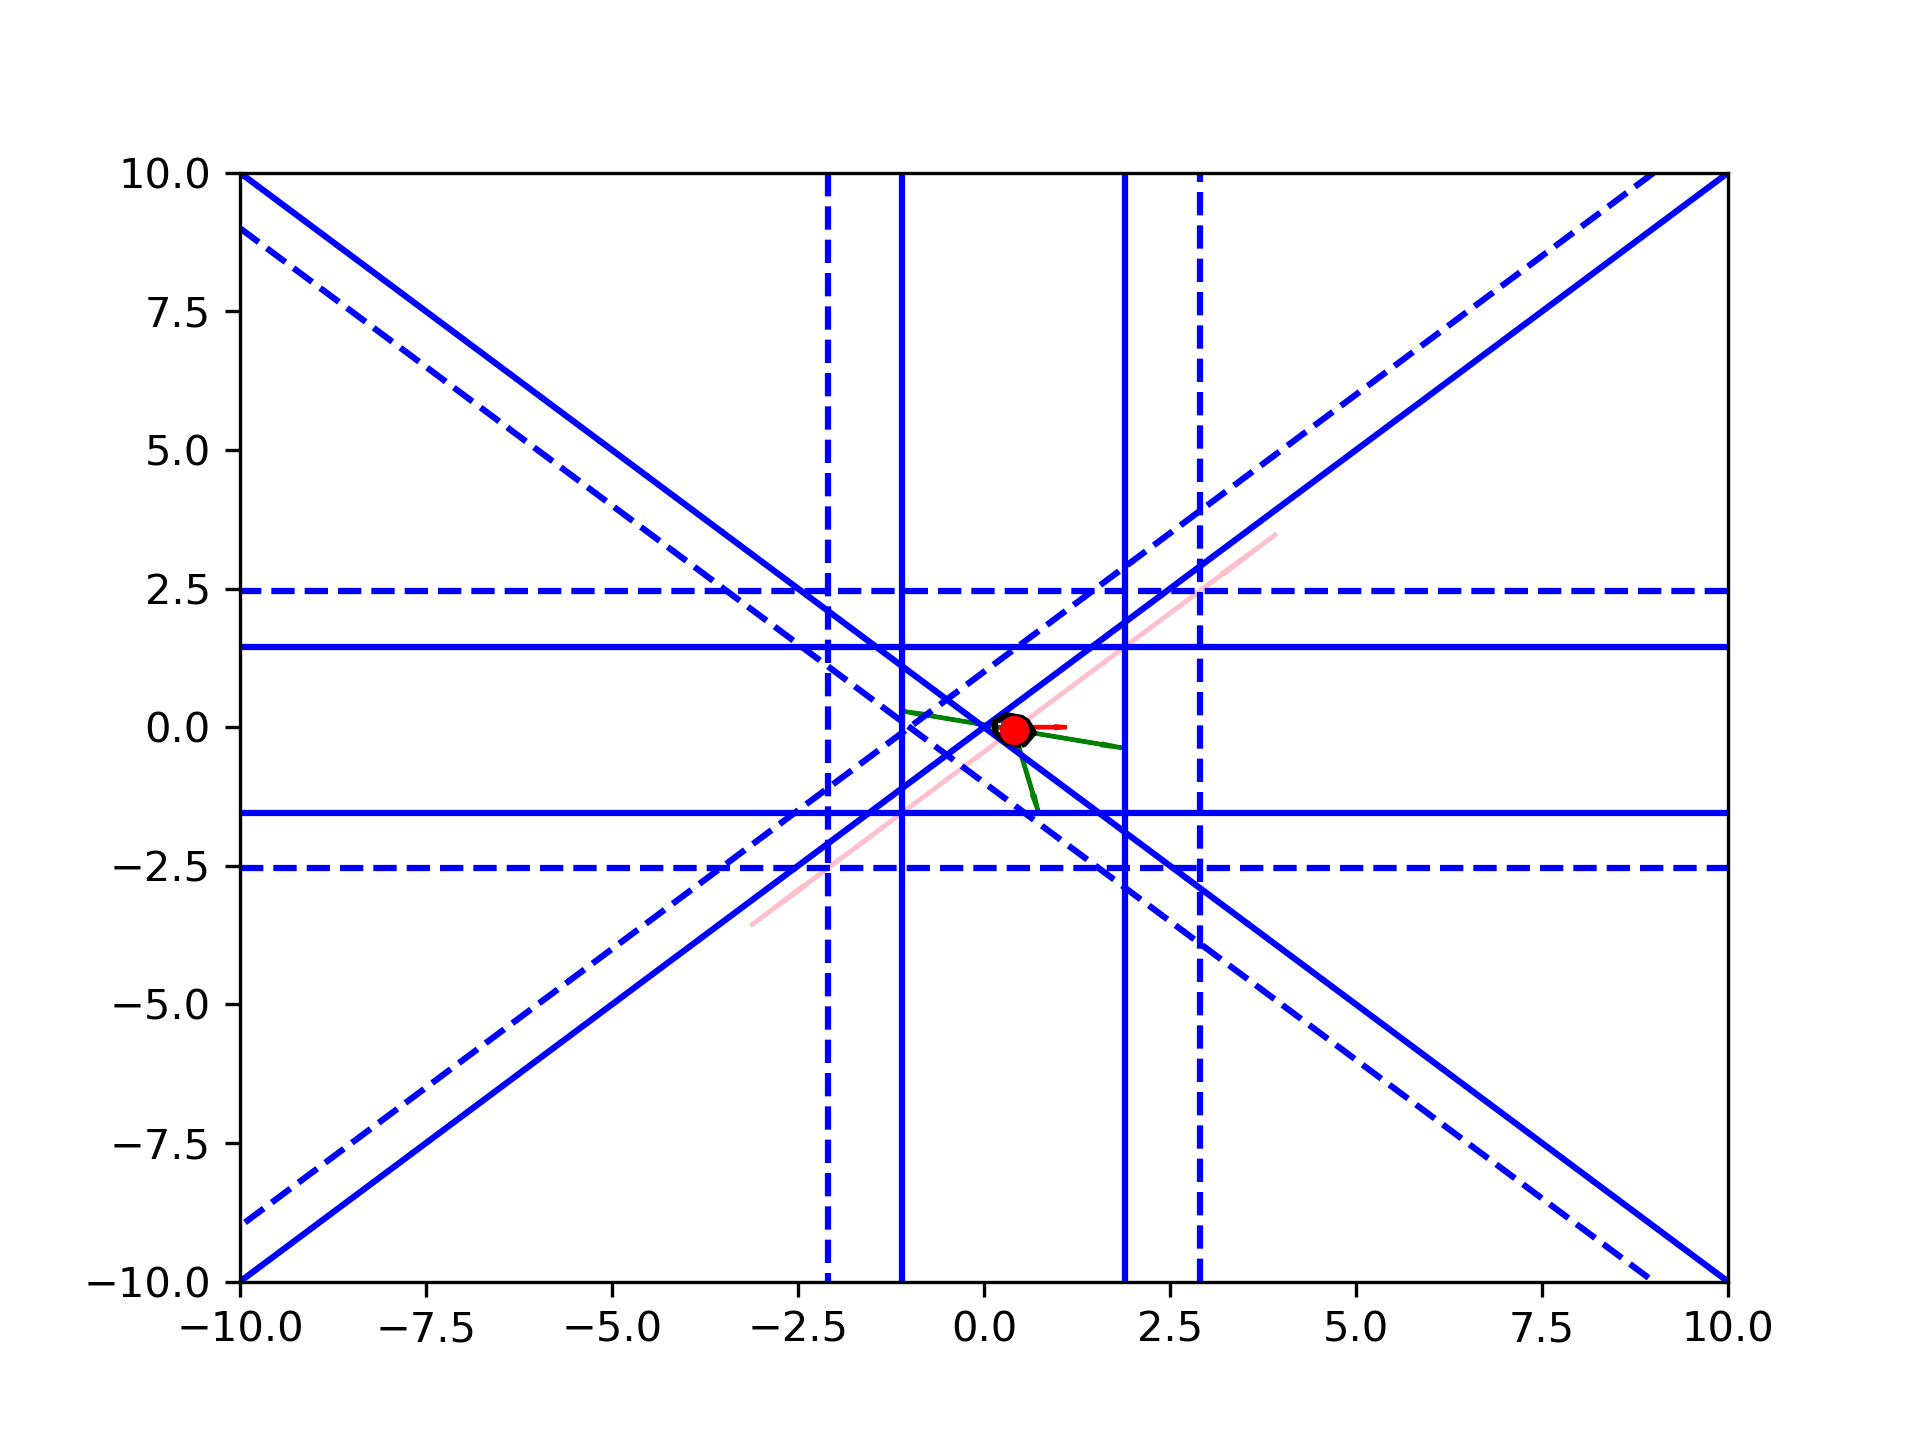
\includegraphics[scale=0.4]{images/everything_runs_1.png}
    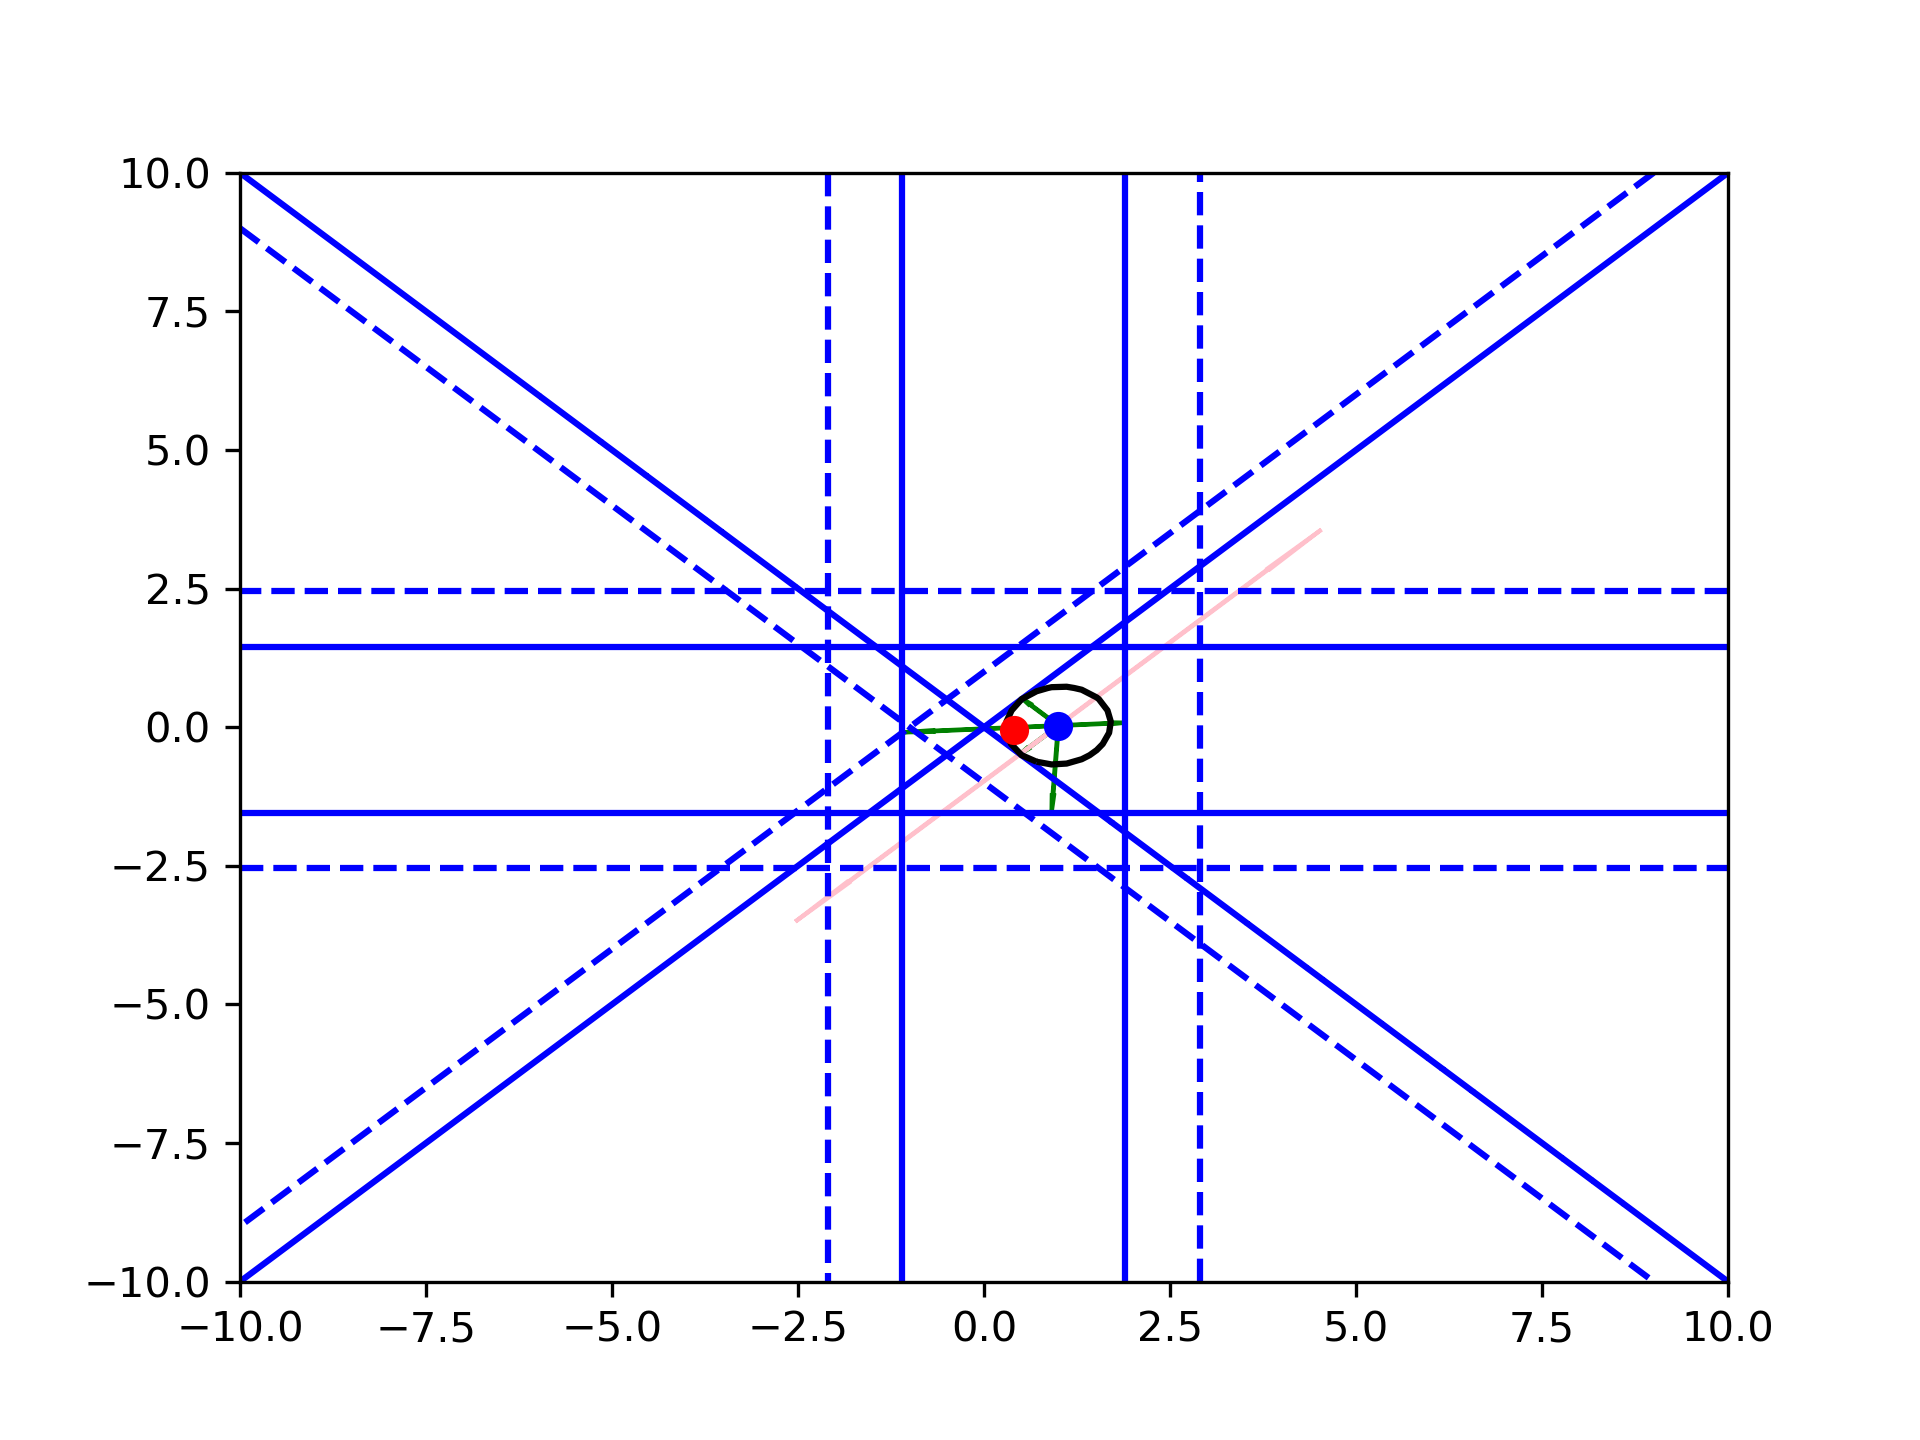
\includegraphics[scale=0.4]{images/everything_runs_2.png}
    \caption{Searching $\feasiblek$}
    \label{ellipse_runs_away}
\end{figure}


One attempt to fix this problem is by limiting the search direction for the center of the ellipse.


\subsubsection{Line searches}
Although $\modelk$'s minimizer over $\outertrk$  can appear anywhere, there are some reasons for expecting it to be at a ``vertex."
If it lies on the interiorer, there is little need for using constrained approaches once near the solution.

The ellipse with maximum volume, however, tends to lead $\innertrk$ away from vertices.
One way of trying to ensure a feasible direction towards a vertex, while still allowing a larger volume ellipse, is by limiting the search for the new center to lie on line segments starting at the current iterate $\iteratek$.

For example, our first attempt was to simply search a line directed away from the closest constraint.
This has obvious problems as shown in figure \ref{first_line_search}, as we should avoid letting the new center get closer to another constraint:

\begin{figure}[h]
    \centering
    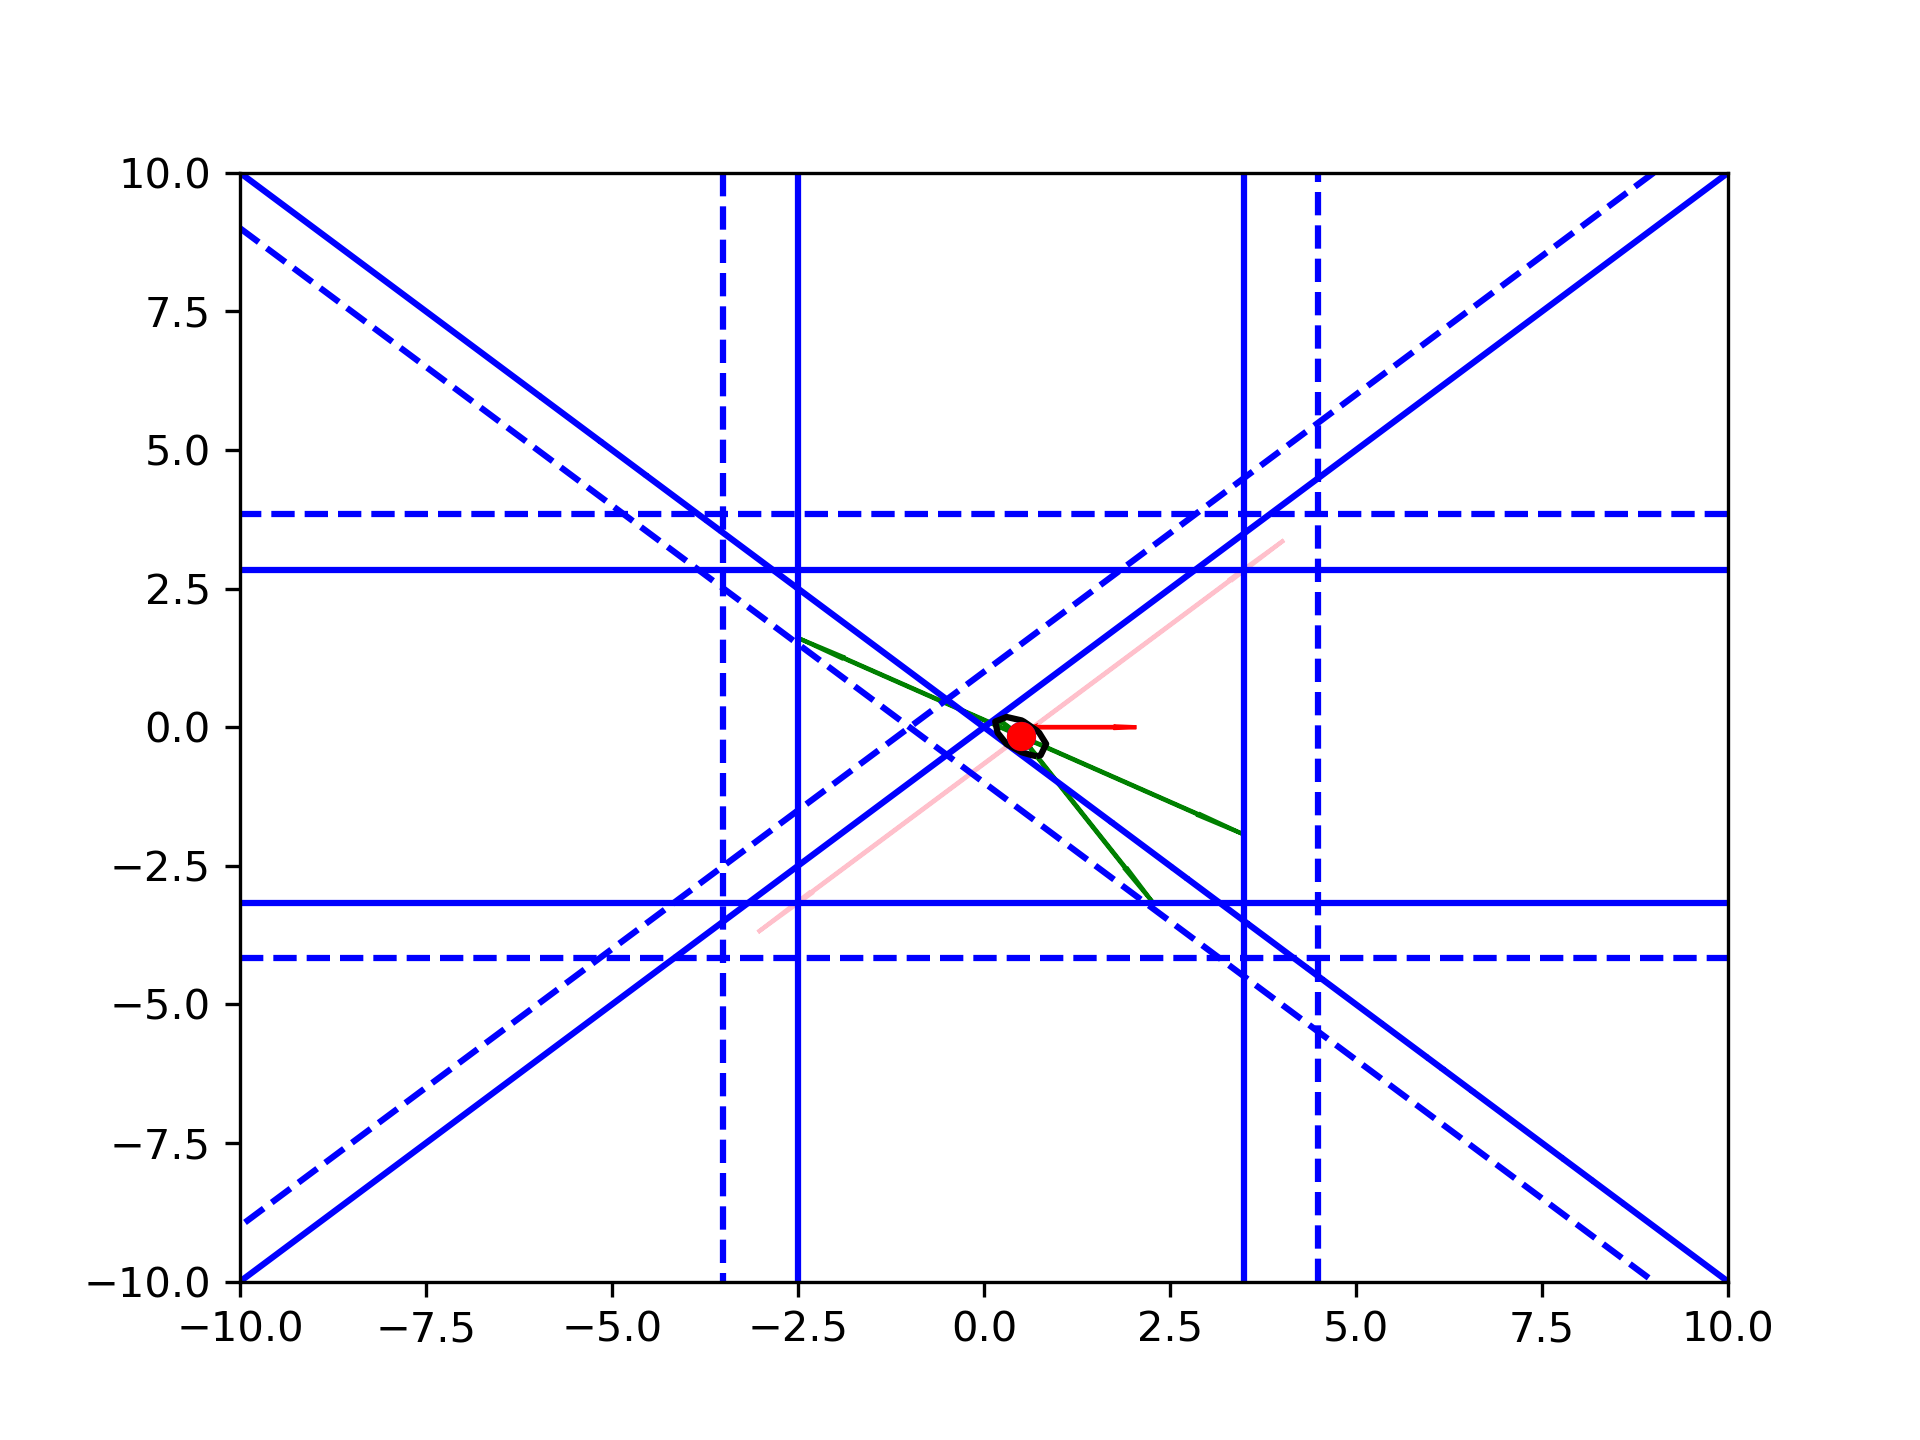
\includegraphics[scale=0.4]{images/line_1.png}
    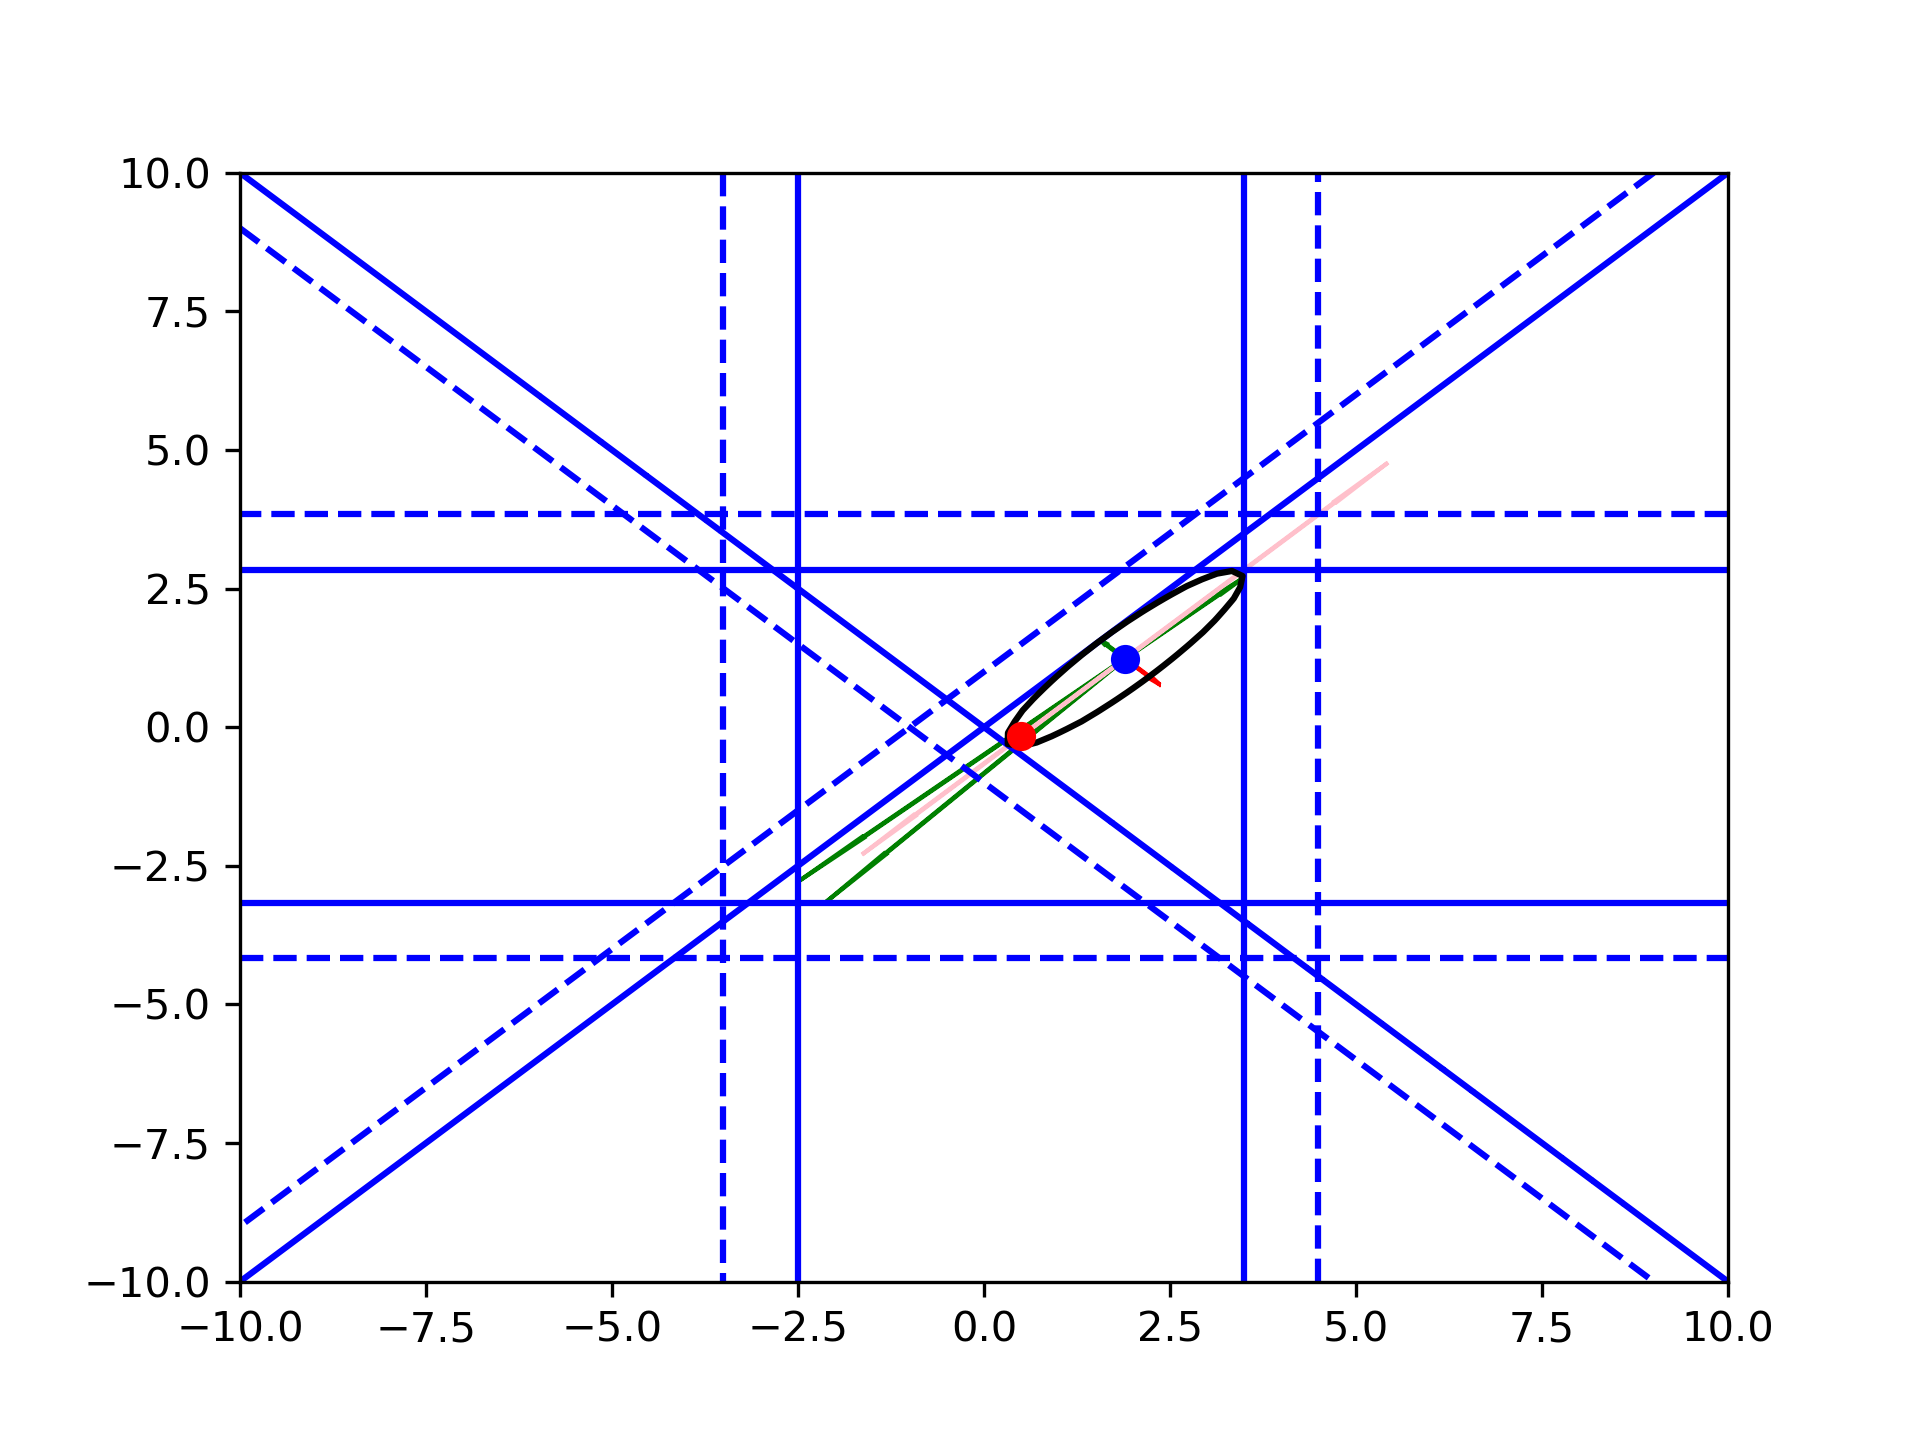
\includegraphics[scale=0.4]{images/line_2.png}
    \caption{Line searches}
    \label{first_line_search}
\end{figure}


To fix this, we break the search path within the \emph{ConstructTrustRegion} subroutine into segments based on the nearest constraint.
We find the center that maximizes the volume of the ellipse after restricting it to lie on a ray perpendicular to the nearest constraint.
Nearest, here, means the constraint with the smallest distance from the iterate to the projection of that iterate onto the constraint:
if we let $\nabla \modelconstrainti(\iteratek) = A_i$ be the $i$ row of $A$, then we define the distance from a search point $s$ so the $i$th constraint to be
$d(A_i, x) = \frac {|A_i x - b|}{\|A_i\|}$.
Let $i$ be such that $d(A_i, \iteratek) \le d(A_j, \iteratek) \; \forall 1\le j\le m$, then we set the first ray direction to be $r_1=-A_j$.
We search along the ray $\{x +tr_1|t\ge 0\}$ from the current iterate until we reach a point $x'$ that also has the same distance to another constraint as the nearest to the iterate:
$\exists j \;s.t.\; d(A_i, x') = d(A_j, x') \le d(A_k, x') \forall 1\le k \le m$.
This completes the first segment.
It can also happen that at the starting point there are two (or even more) constraints that are both closer than all others, say there are some $1\le i,j\le m$ with $d(A_i, \iteratek) = d(A_j, \iteratek) \le d(A_k, \iteratek)  \forall 1\le k \le m$.
In this case we simply follow a ray whose points are equidistant from both of these constraints: $\{x - t\frac 1 2 (A_i + A_j)| t \ge 0\}$.
At the end of each segment, we construct a ray that is equidistant to all constraints previously encountered.
We could then, in general, continue to follow line segments by always travelling away from the nearest constraints until we reach a point equidistant to $n+1$ constraints.
However, after we include enough constraints, we will eventually once again head away from a vertex.

This means that we can define a class of searches that each limit the number of line segments to search.
In this paper, we consider searches with one and two line segments for $\mathbb R^2$.
In figure \ref{line_can_run}, the red line shows the line segments maintaining equidistance to their closest constraints.
Notice that with two line segments, the algorithm can already choose new centers further from the vertex.

% TODO: REPLACE PICTURES
\begin{figure}[h]
    \centering
    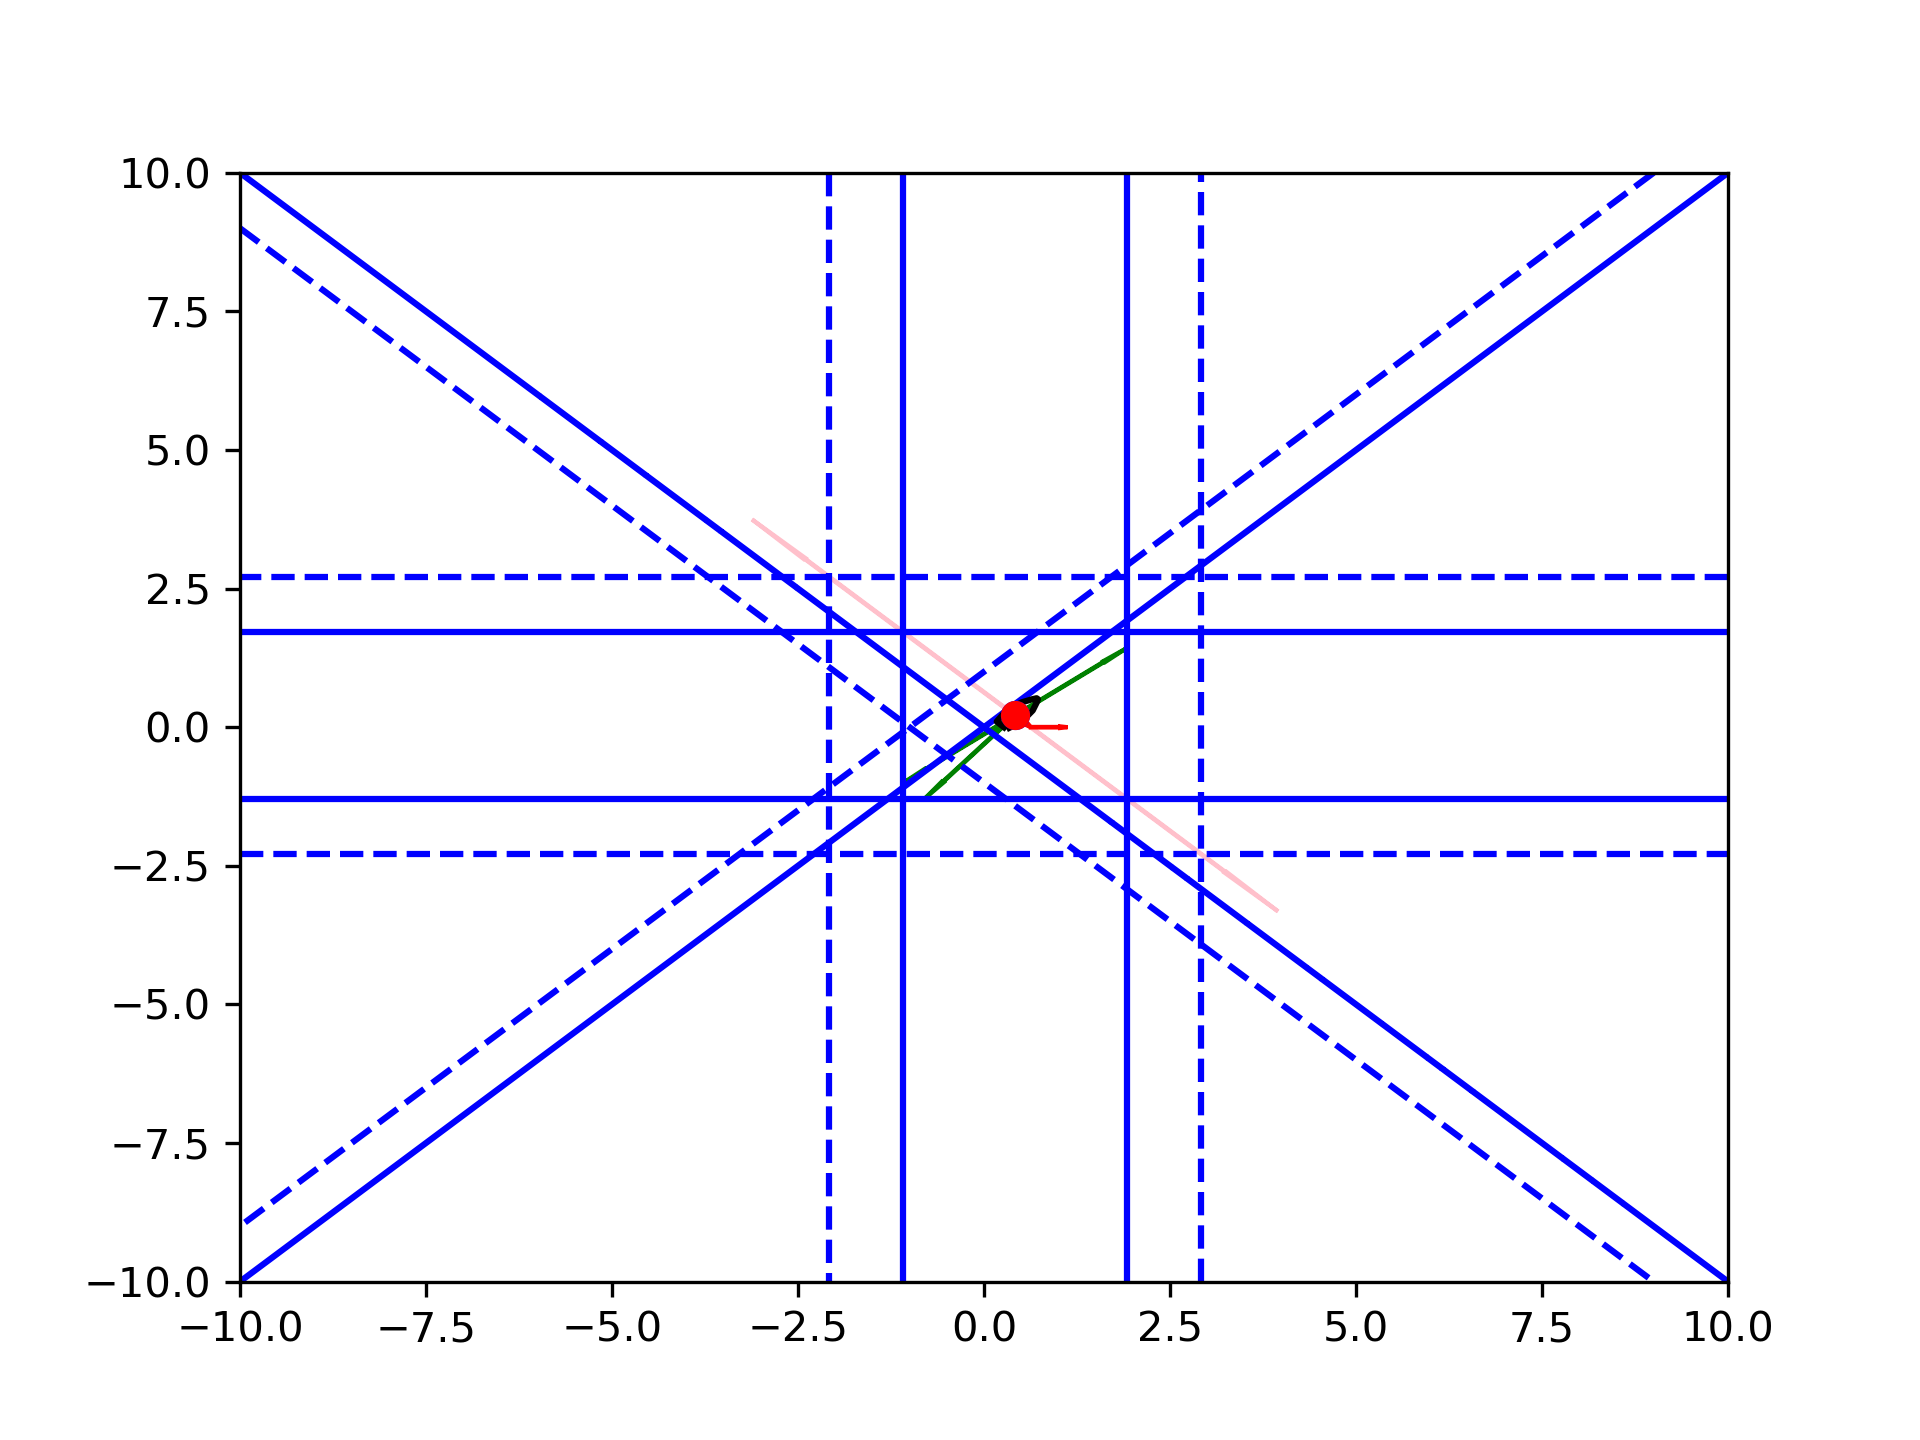
\includegraphics[scale=0.4]{images/run_away_1.png}
    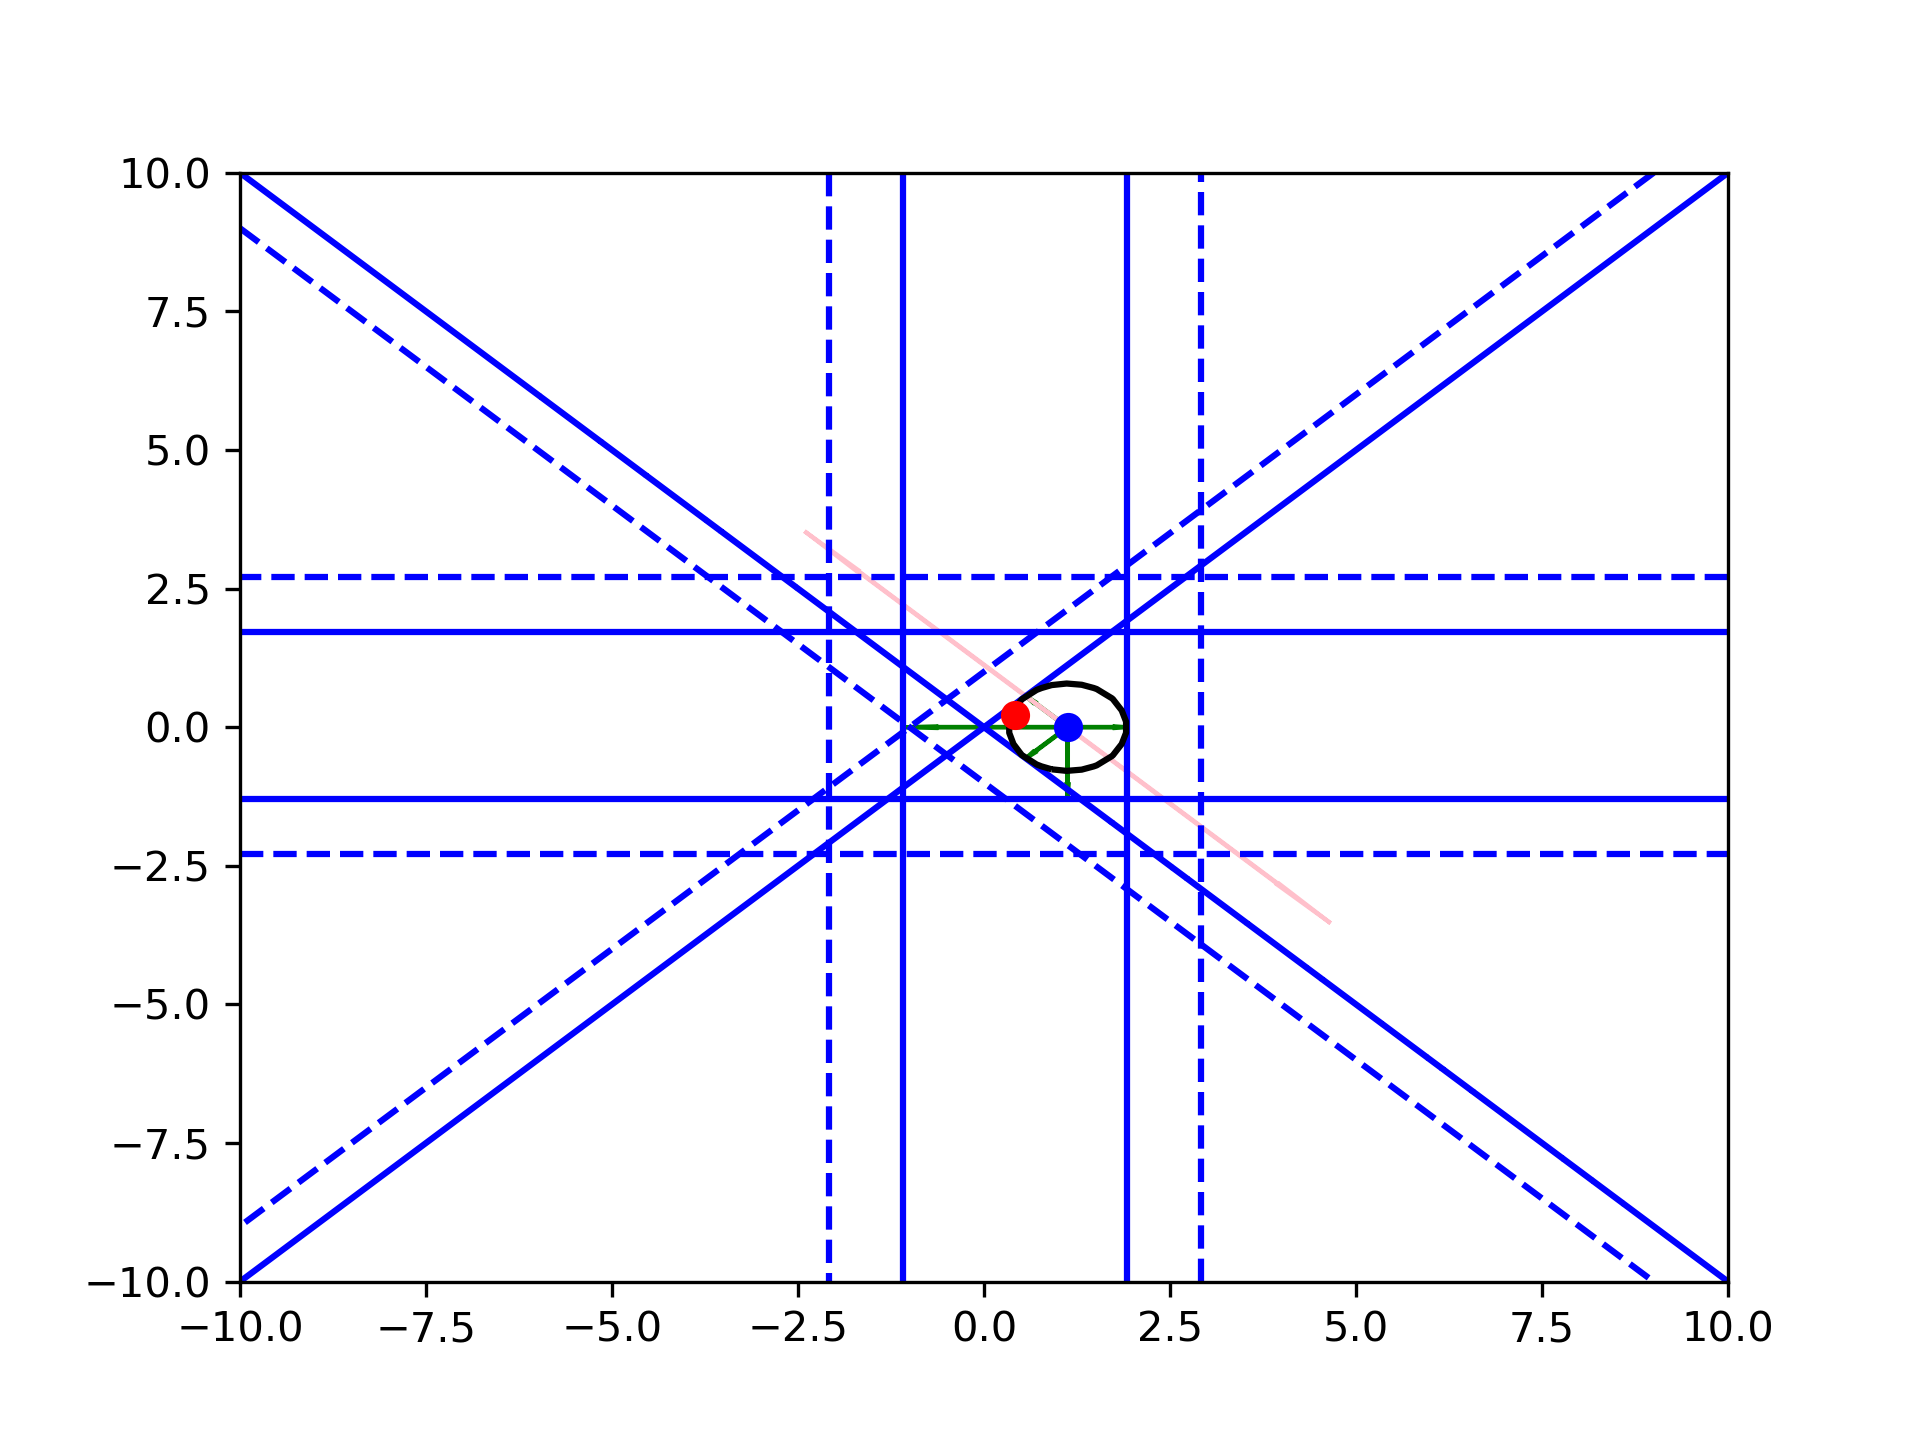
\includegraphics[scale=0.4]{images/run_away_2.png}
    \caption{Ellipse runs away from the optimizer}
    \label{line_can_run}
\end{figure}


\subsubsection{Hueristically Good Ellipsoid}

It may be possible to encourage the ellipse along the desired direction while still maintaining a large enough volume if we include information from the current model functions.
Among the desirable traits for the new ellipse, we would like:
\begin{itemize}
    \item The ellipse should not only have a large volume, but that volume should be distributed where the next iterate is likely to lie
    \item The ellipse should reuse as many sample points from the previous iterate as possible.
\end{itemize}


%By Lemma $3.7$ of \cite{DUMMY:intro_book} pp. 45 we know that the model will be poised for any subset.

In order to address the first item, we developed a hueristic to increase $\mathbb P(s^{(k)} \in E_k)$.
In order to do this, we use the previous model function as a baseline for where the next trial point is likely to lie.
There are several ways to add variance around this model to account for innacuracy, including quadratic, linear, or kriging bounds.
The way we have implemented is using a set of interpolation functions as possible errors.
One such set of error functions $\phi^{\epsilon}_i$ are higher order polynomials.
In figure \ref{smf}, we use two cubic terms in addition to the quadratic models.
We extend the vandermode matrix in \ref{reg} to include terms of the error interpolation functions, however we do not force the the lagrange property on these functions.
Instead, we compute the null space of $V$ to have a basis for all error interpolation functions such that $\phi^{\epsilon}_i(y^j) = 0 \forall i,j$.

By sampling these error functions, we are able to create a distribution of possible trial points.
For example, in the following images, the true objective is black, the trust region is green, the model function is blue, and the sampled model function is red.
The current model function's minimizer is magenta, while the sampled model function's minimimzer is yellow.

\begin{figure}[h]
    \centering
    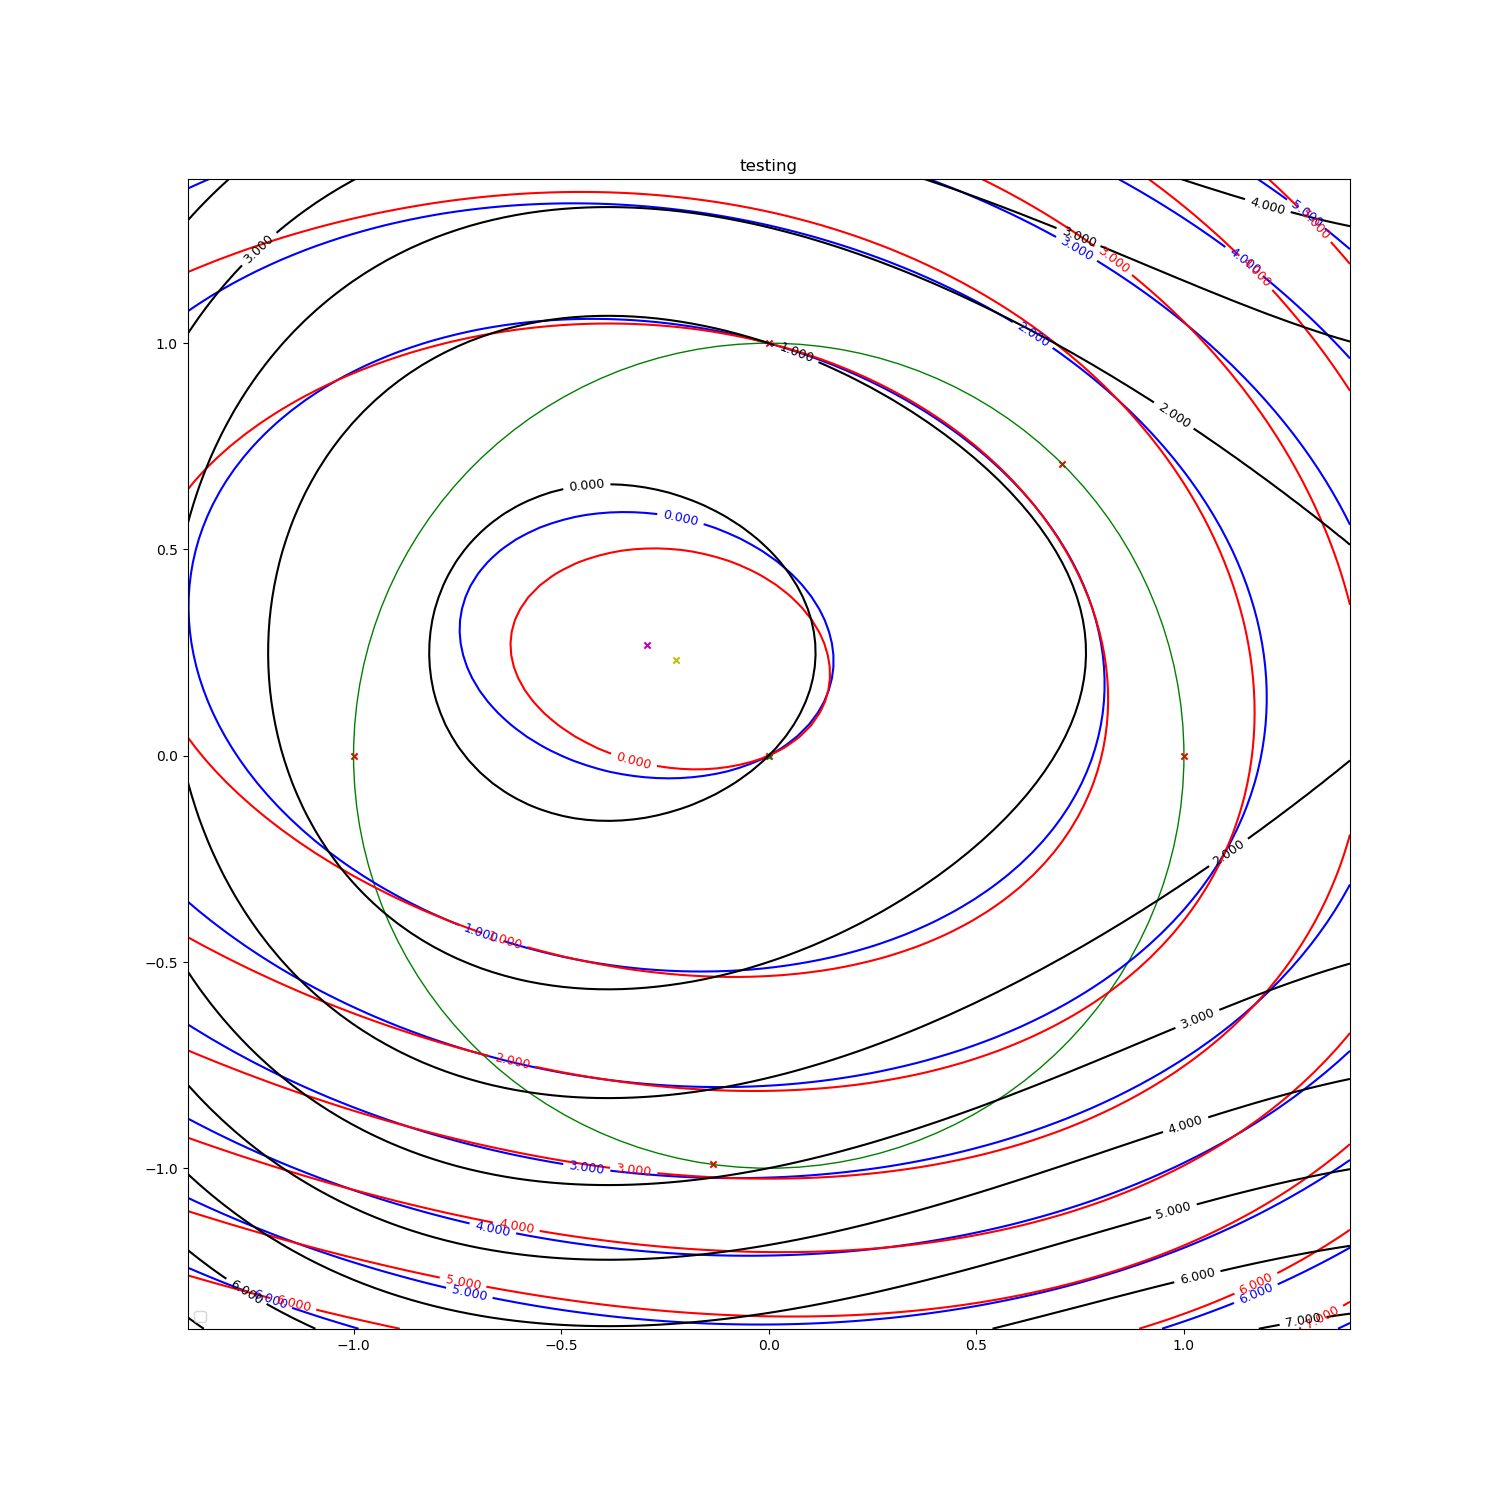
\includegraphics[width=125px]{images/other_polynomial_2.png}
    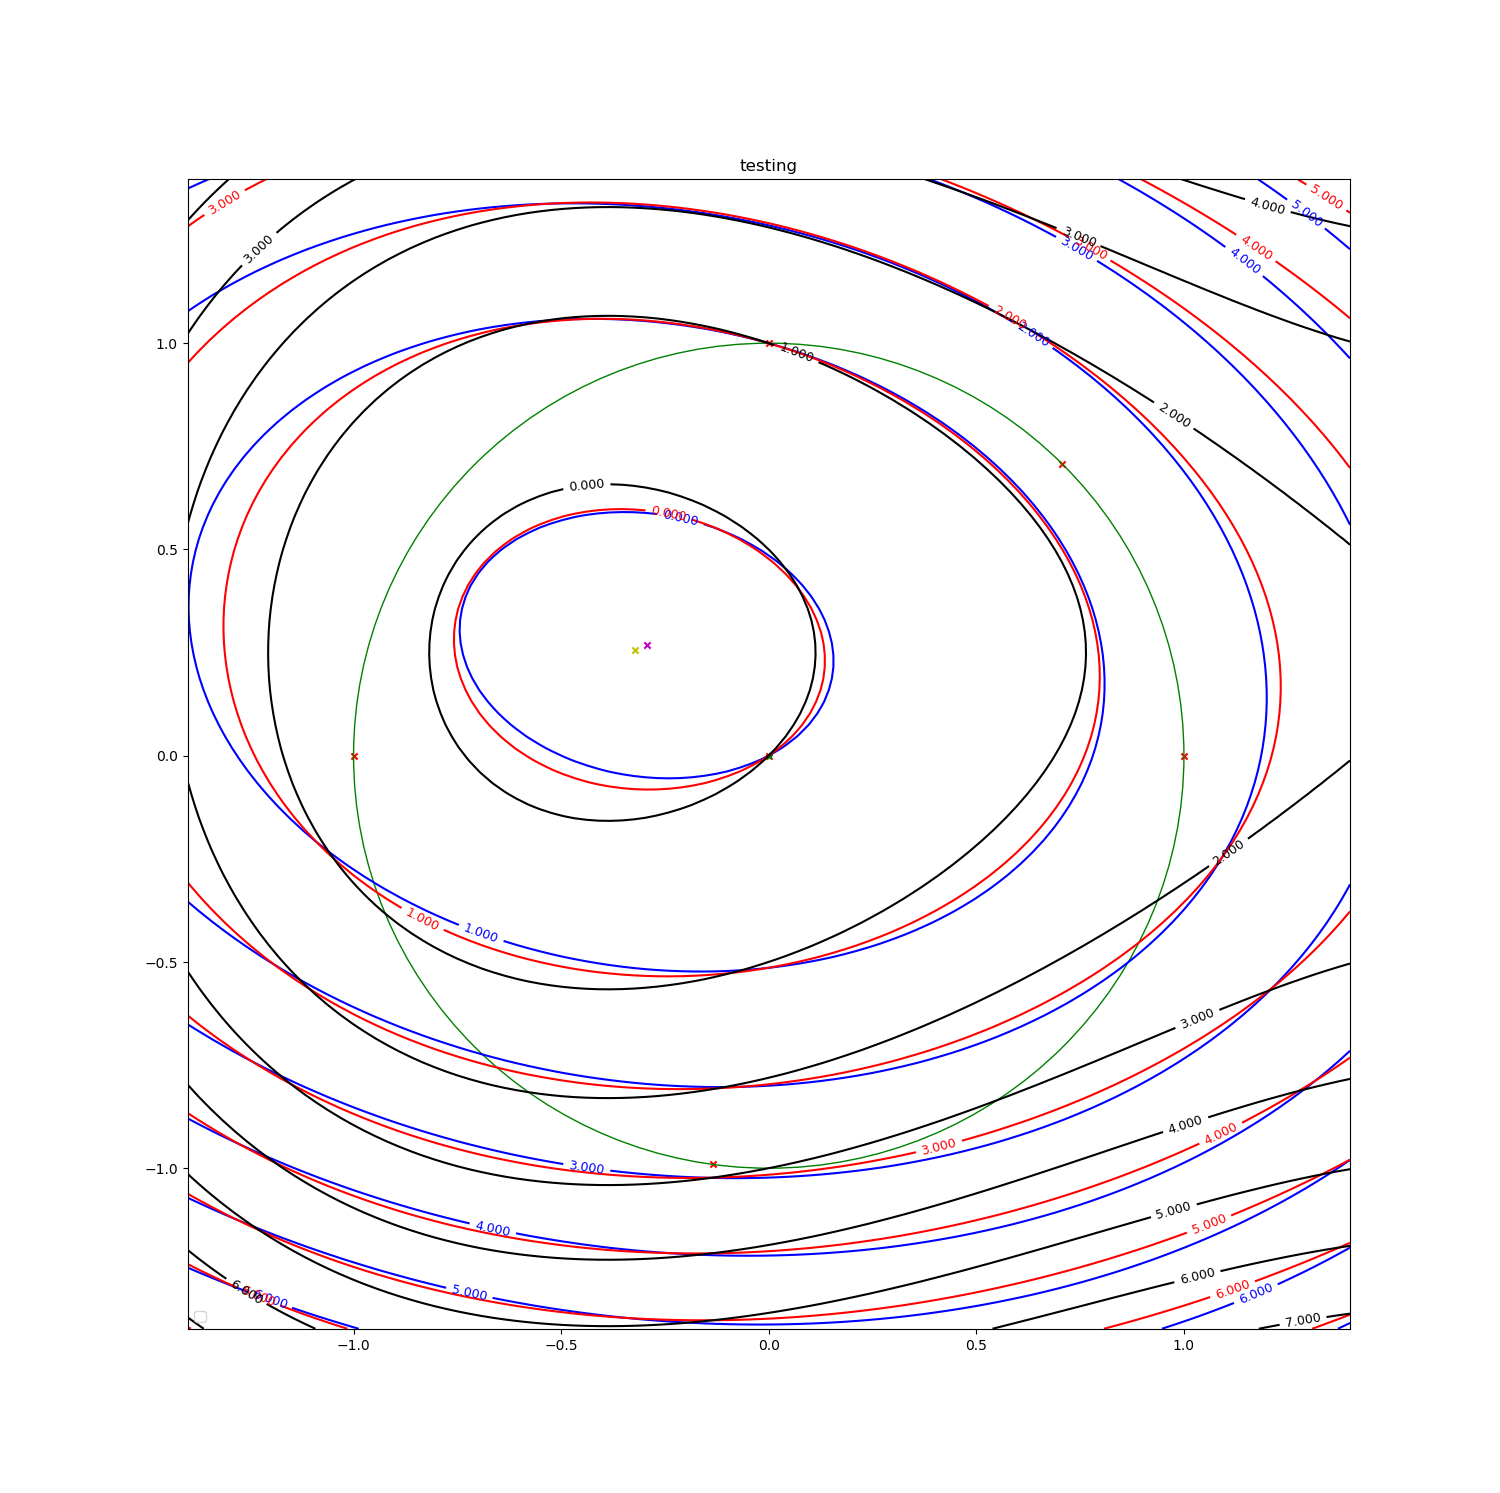
\includegraphics[width=125px]{images/other_polynomial_3.png}
    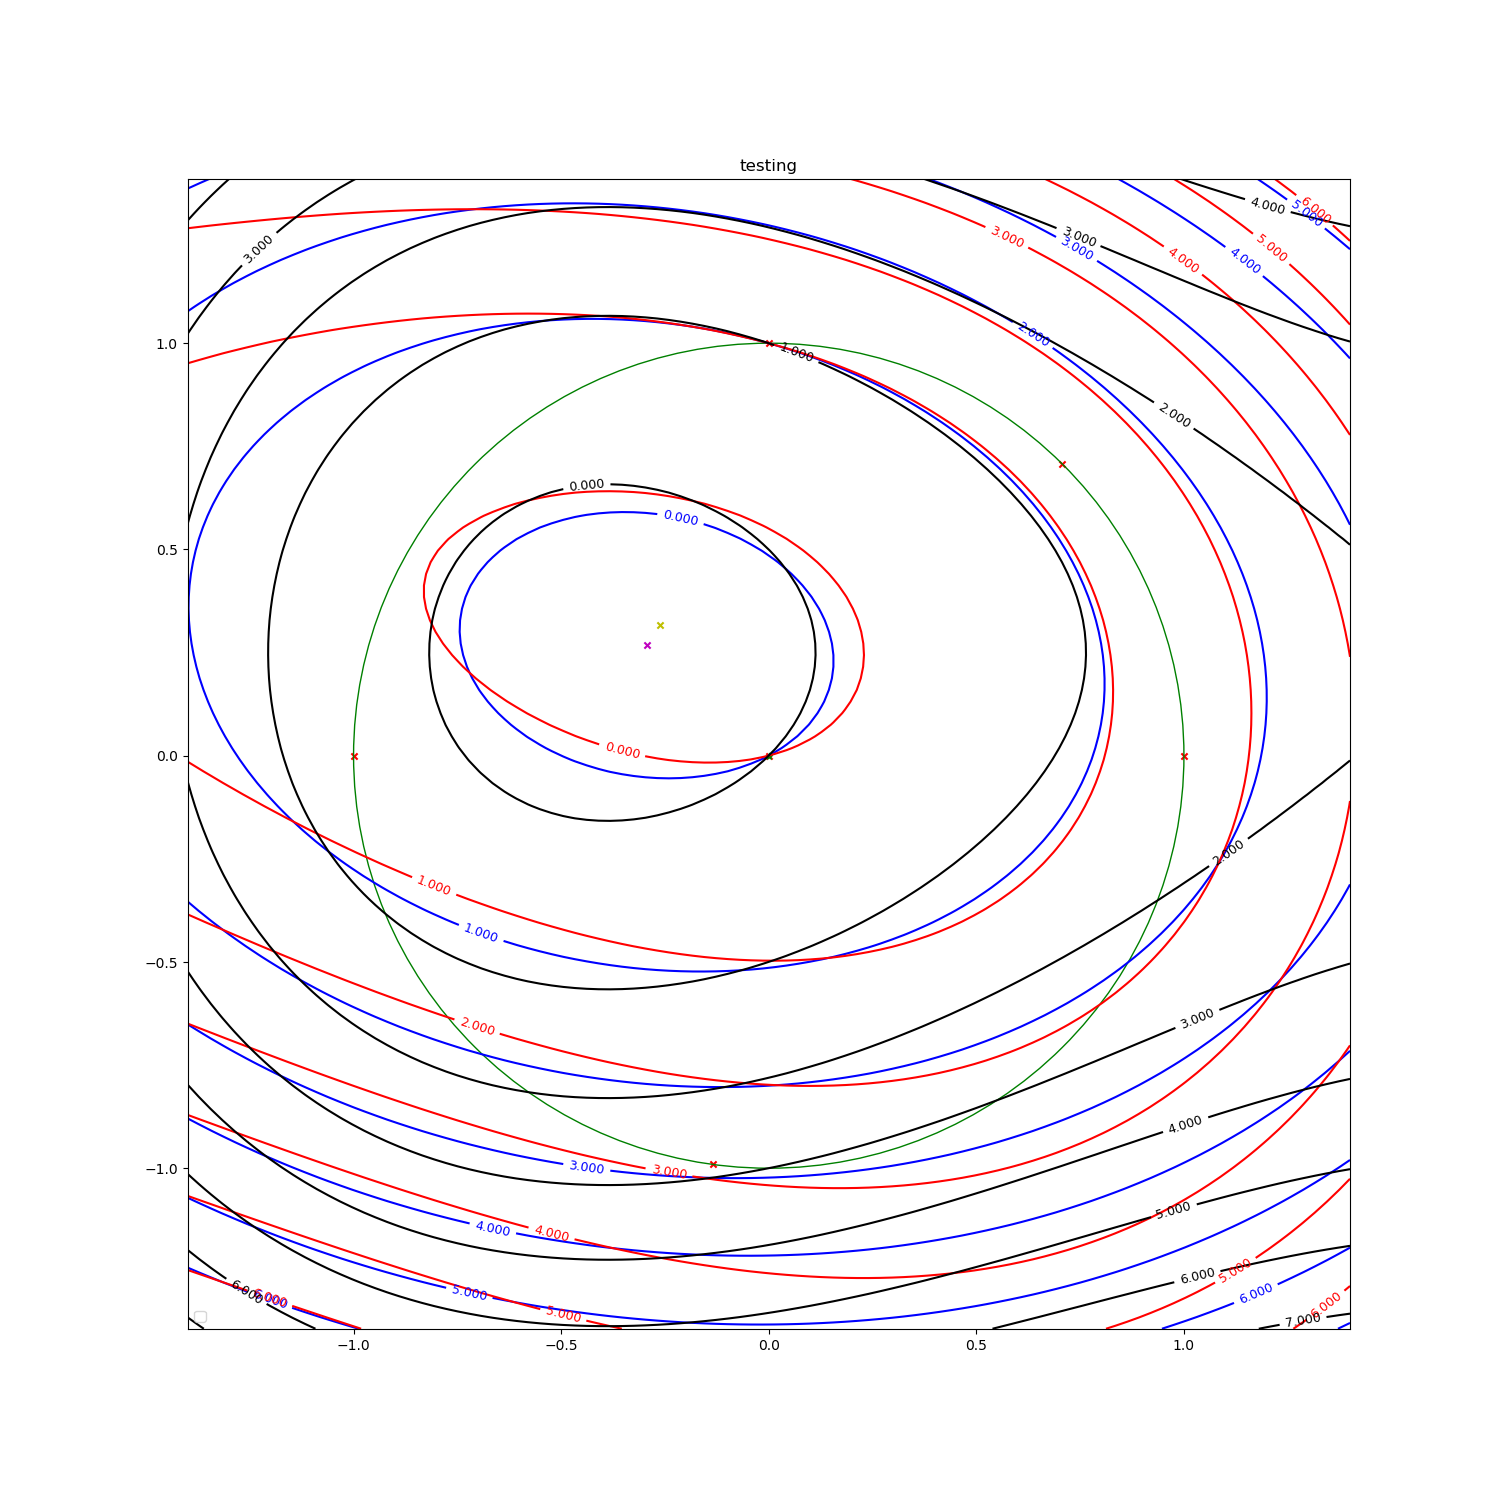
\includegraphics[width=125px]{images/other_polynomial_5.png}
    \caption{Sample model functions}
    \label{smf}
\end{figure}

We repeatedly sample the model function $N$, and compute its minimizer.
Collecting these minimizers $h_i$ produces a heuristic distribution of where the next trial point is likely to lie:

\begin{center}
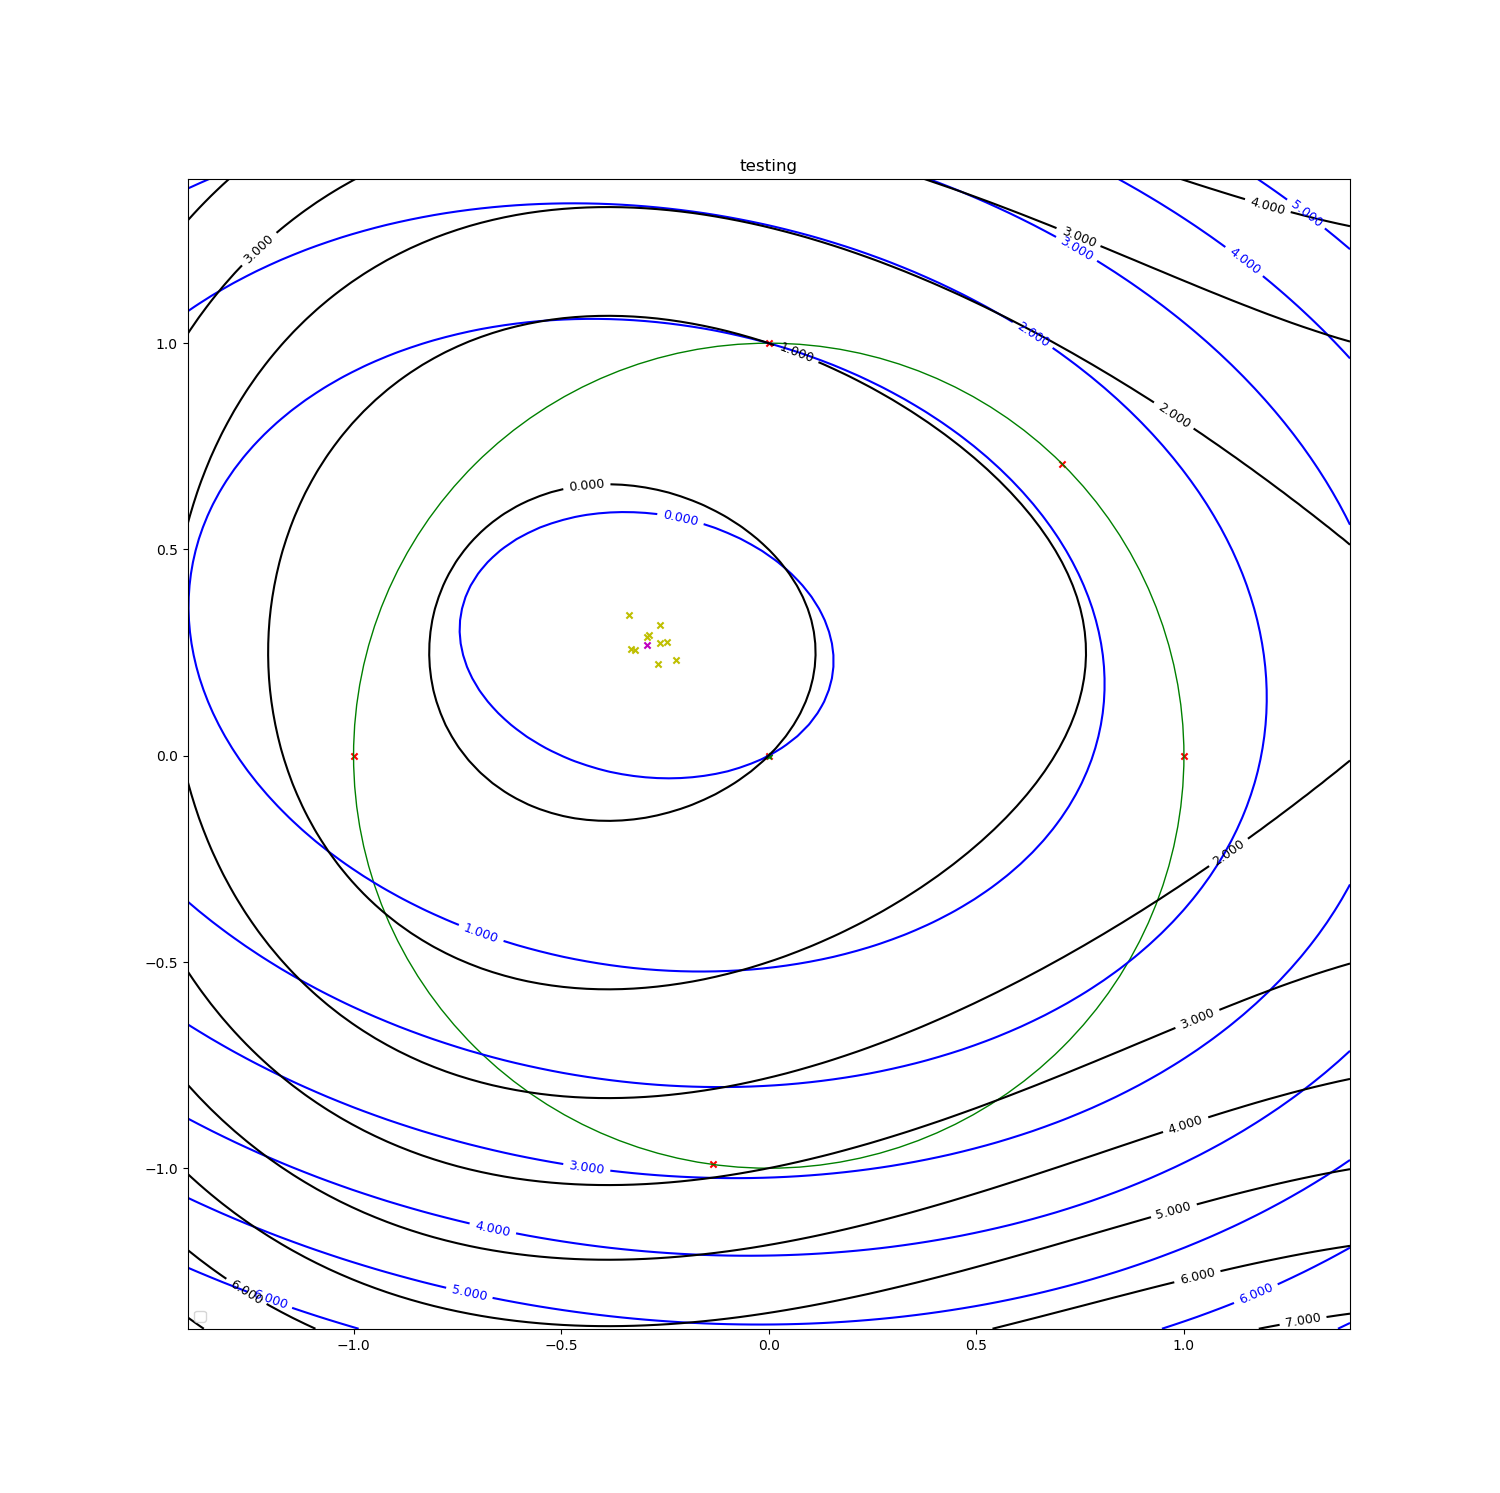
\includegraphics[width=200px]{images/sampled_minimums.png}
\end{center}

We can then set our heuristic $H$ to be $H(E_k) = (\int_{x\in \outertrk} \frac 1 N \sum_{h_i}r(\|x - h_i\| dx)$,
where $r(0) = 1$ and $x>0 \Rightarrow r'(x) < 0$.

This produces the value plot in figure \ref{hvalueplot}, where the magenta contours represent the value of including these points, the green ellipse is the previous trust region, the black lines are the current constraints, and the blue contours are the previous model function.

\begin{figure}[h]
    \centering
    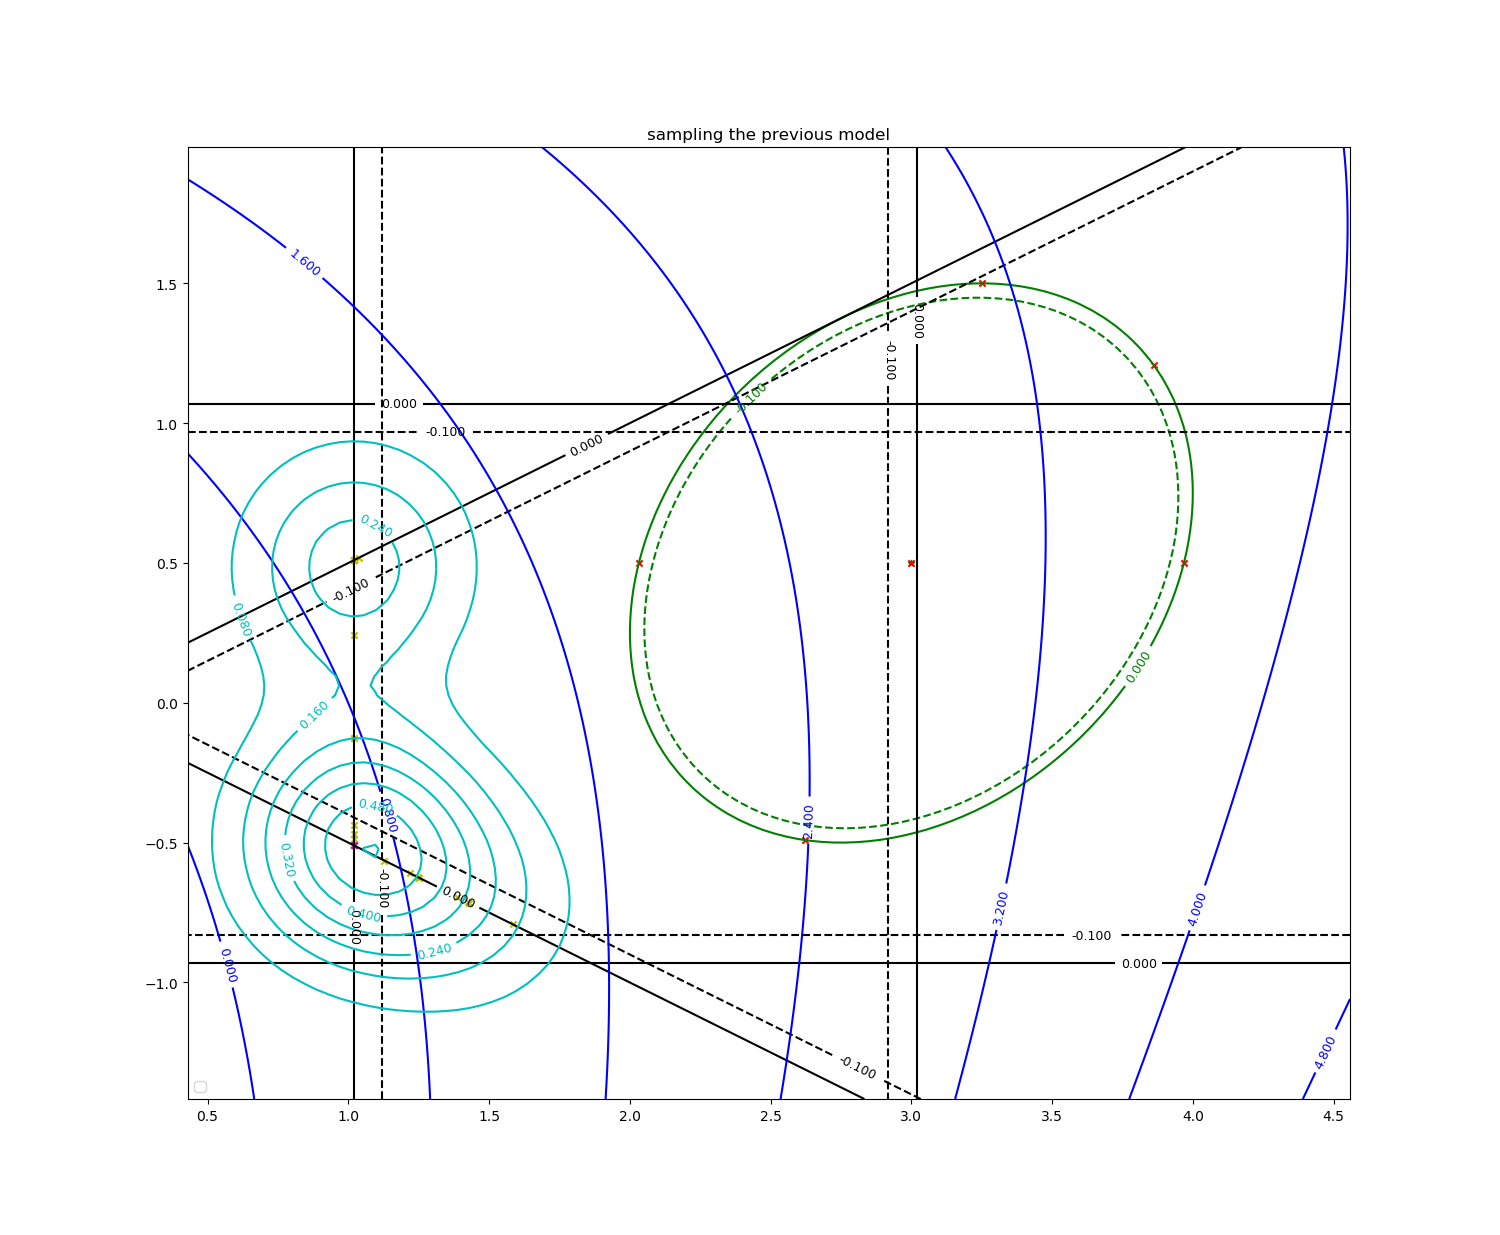
\includegraphics[width=200px]{images/heuristic_value.png}
    \caption{Heuristic value}
    \label{hvalueplot}
\end{figure}



While sampling other model functions, we sample with mean $0$ to ensure that the current model function is most likely.
However, we set the variance of the sampling distribution based on the previous models error:
$\epsilon_k = |\modelkmone(\iteratek) - \modelk(\iteratek)| = |\modelkmone(\iteratek) - f(\iteratek)|$.
We ensure that with fixed probability $p_0$, the sampled model functions have error less than this error at the models best guess for the next minimum.

Without much tuning, this has already improved the ellipsoid searched over the entire trust region.
This distribution may also be useful for decreasing the trust region radius more quickly.


\subsubsection{Subsets of the Trust Region}
\label{simplex_subset_algorithm}

This is another approach to ensuring \ref{accuracy} of the model functions when using the bumping $\xi$ strategy.
Suppose that at some point we are not able to find a sample point passing \ref{impossibly_poised}.
The following idea is based on the fact that if we cannot find a set of sample points poised over then entire polyhedron, they will still be poised over their own convex hull.

Although not computationally feasible for when $A$ has a large number of rows, we are able to sample simplexes to find one containing both the current iterate and likely to contain a descent direction.

\begin{algorithmic}
\Procedure{Volume}{$S$}
    \State \textbf{return} $\frac 1 {n!} \det{[S_1 - S_0, \ldots, S_n - S_0]}$
\EndProcedure
\Procedure{ConstructTrustRegion}{}
    \State $T_{\text{best}} = \emptyset$
    \State $V_{\text{best}} = 0$
    \ForAll{$S \subset \outertrk \cap X$ a simplex}
        \If{$x^{(k)} \not \in S$}
            \State{\textbf{Continue}}
        \EndIf
        \If{$diam(S) < \Delta_k$}
            \State{\textbf{Continue}}
        \EndIf
        \State $V_{\text{trial}} = $ \Call{Volume}{$S$}
        \If{$V_{\text{trial}} > V_{\text{best}}$}
            \State $T_{\text{best}} = S$
            \State $V_{\text{best}} = V_{\text{trial}}$
        \EndIf{}
    \EndFor
    \State \textbf{return} $T_{\text{best}}$
\EndProcedure
\end{algorithmic}


Finding the maximal volume sub-polyhedron is NP-hard, but heuristics can be used to modify one easily computable simplex containing $\iteratek$.
Note that we could apply the heuristic used to look for a ellipsoids within this subroutine as well.

In figure \ref{simplex_iterations}, the left image shows the current constraints and trust region, while the second shows the search for the best simplex containing the model center.
Yellow lines are trial simplexes, while the green simplex has the maximum volume.

\begin{figure}[h]
    \centering
    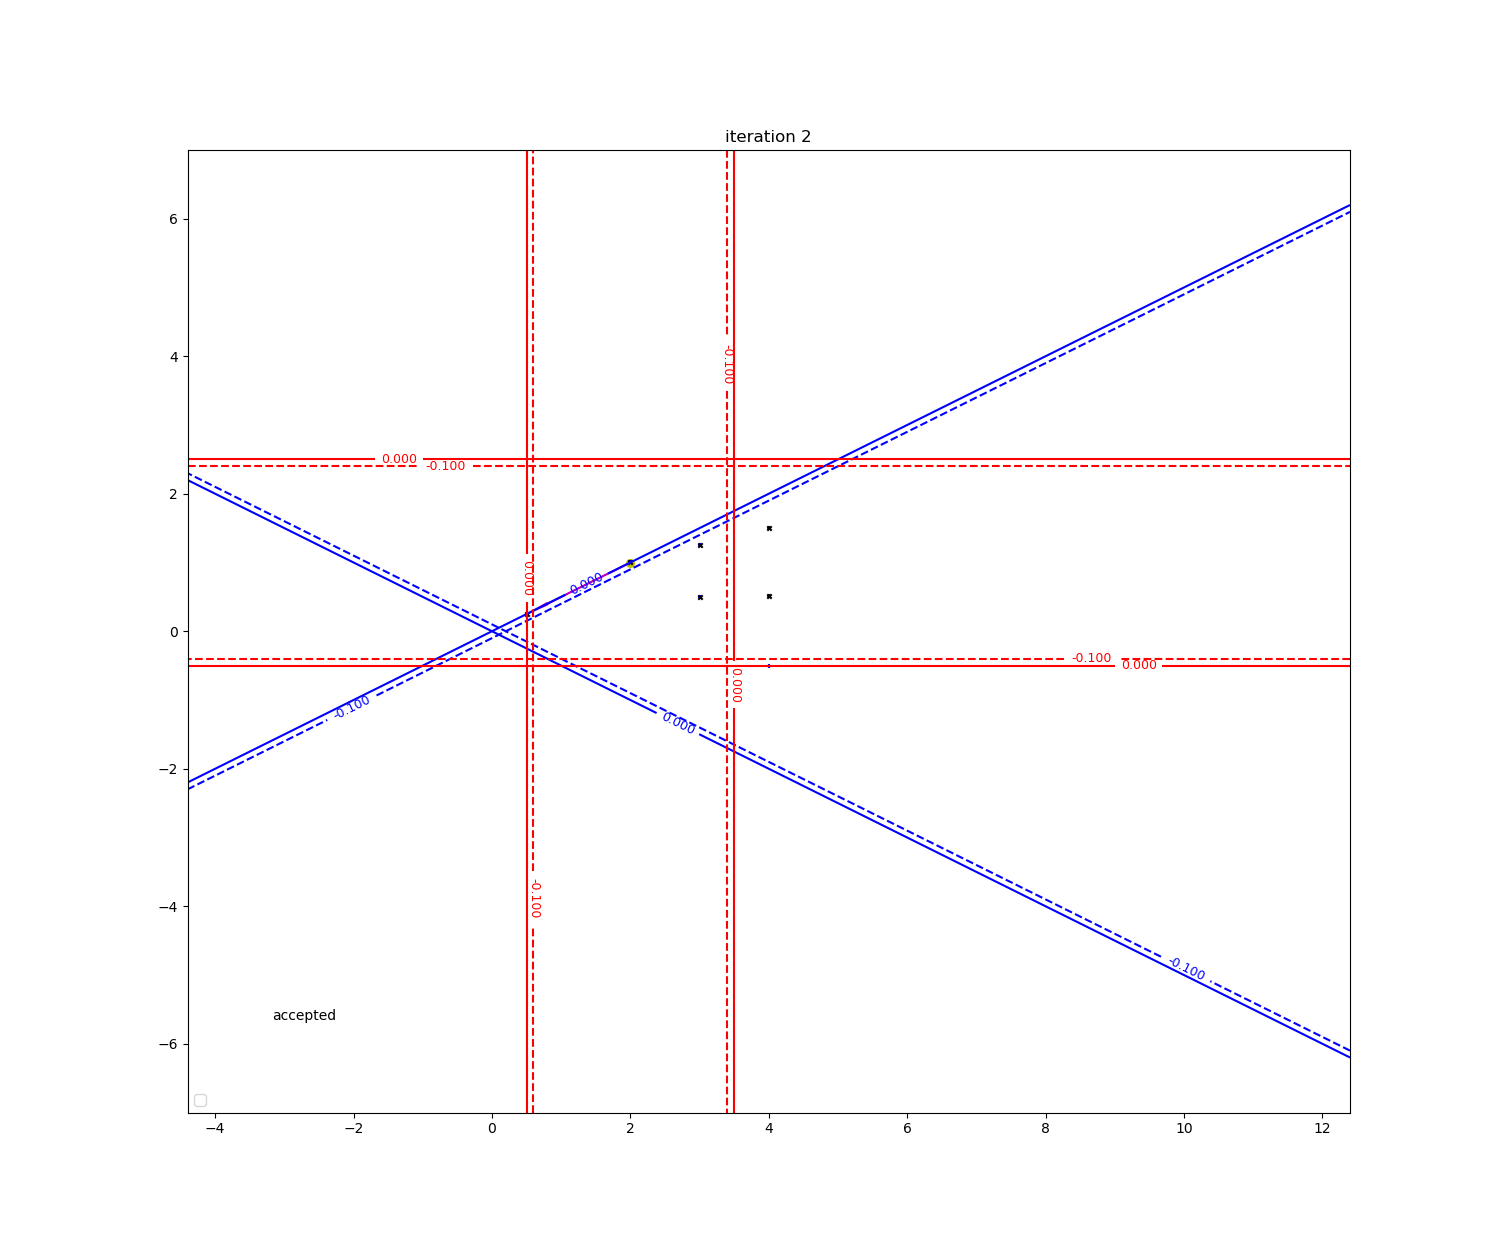
\includegraphics[width=200px]{images/simplex_iteration.png}
    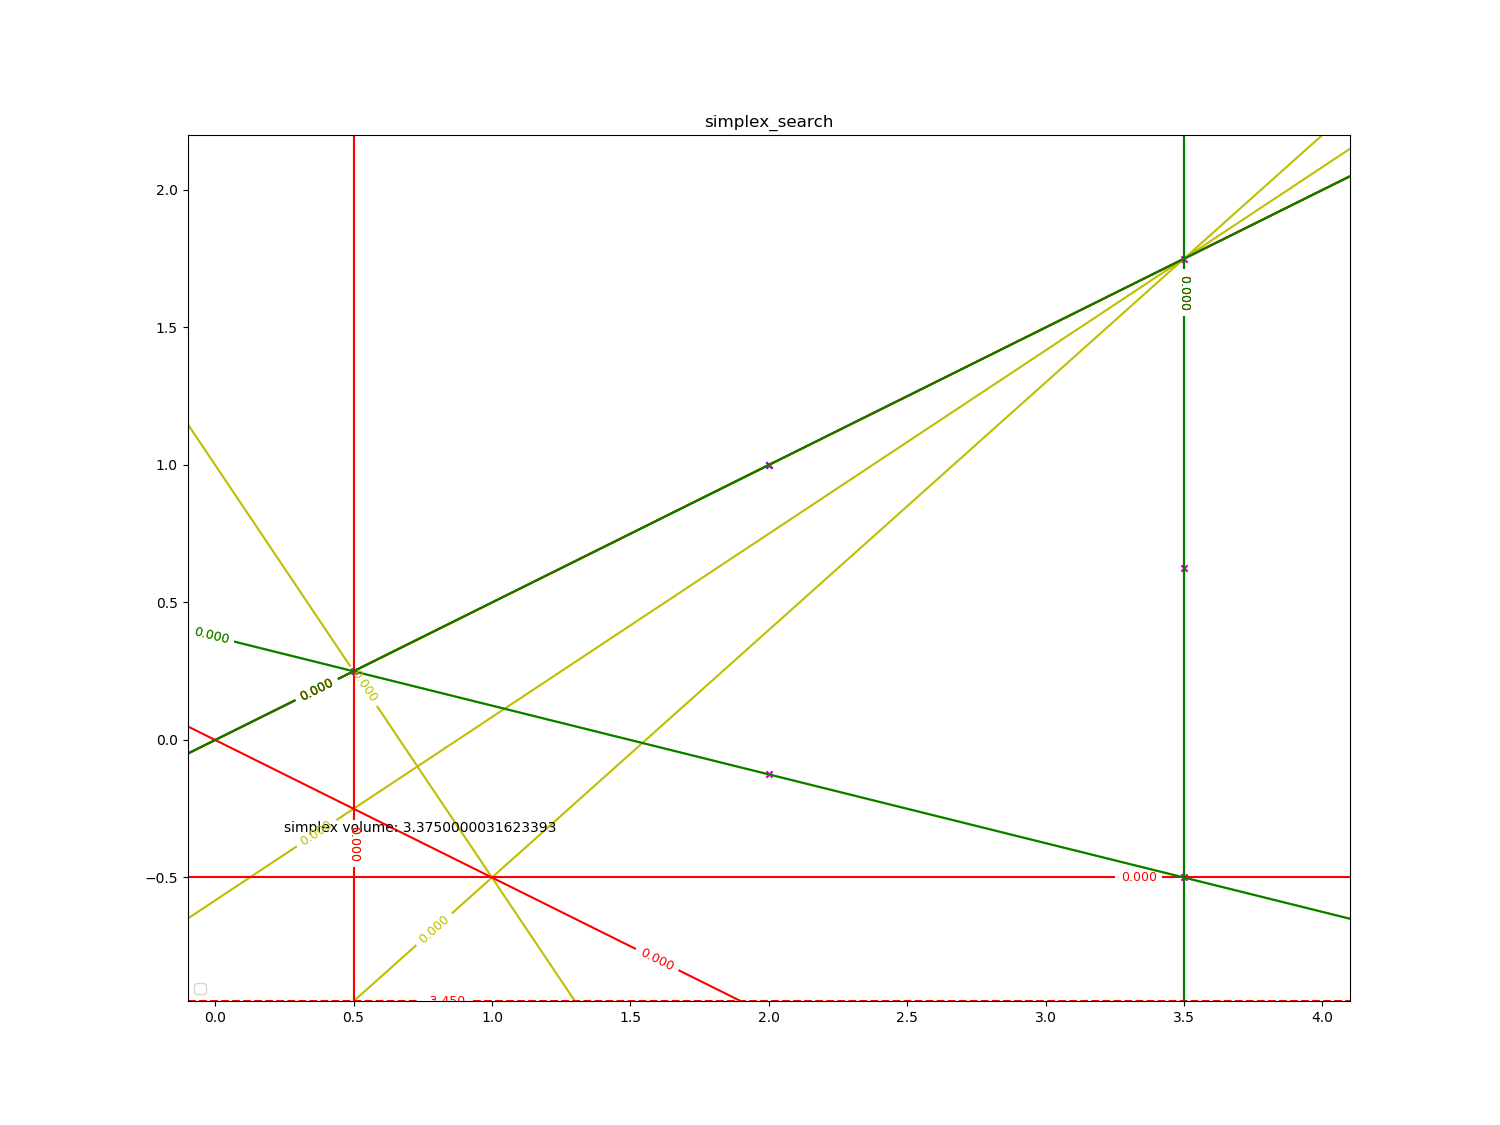
\includegraphics[width=200px]{images/simplex_search.png}
    \caption{Simplex iteration}
    \label{simplex_iterations}
\end{figure}

\subsection{Circumscribed Ellipse}

Another search type we can perform is find the minimum volume ellispe containing all vertices of $\domain \cap T_k$.
In practice, this is very similar to the bumping $\xi$ strategy because the same constraints must be included within the trust region subproblm.
However, the method may be more likely to include previously evaluated points, and we conceptually ``trust"  points over a larger volume.
An example iteration can be seen in figure \ref{circumscribed_ellipse}:


\begin{figure}[h]
    \centering
    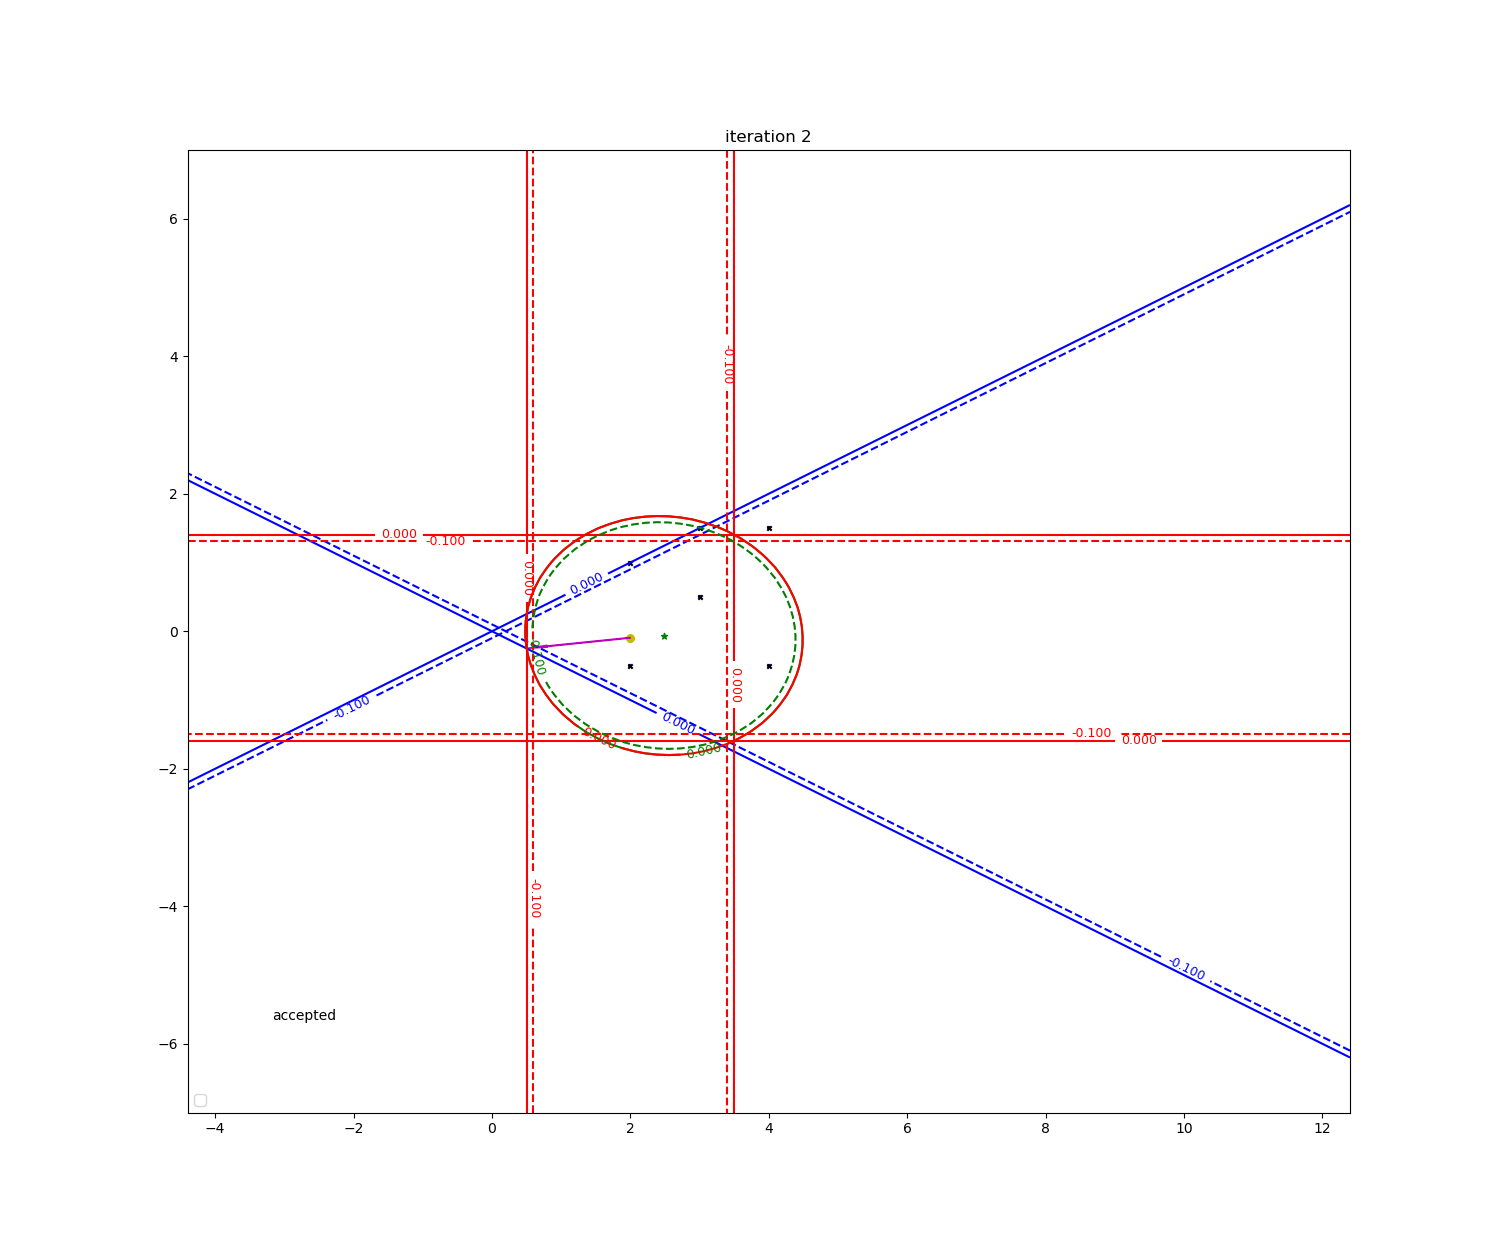
\includegraphics[width=200px]{images/circumscribed_ellipse.png}
    \caption{Circumscribed ellipse}
    \label{circumscribed_ellipse}
\end{figure}


\section{Analysis}

We plan to leverage convergence results found in \cite{Conejo:2013:GCT:2620806.2621814} which presents very general global convergence results for derivative free algorithms over convex constraints.
A key step in showing using this proof will be satisfying the efficiency condition \ref{efficiency} and the accuracy condition \ref{accuracy}.
If the search space within the trust region subproblem is limited to the inner trust region, than we may have difficulty satisfying \ref{efficiency}.


Once these conditions are satisfied, the remainder of the proof can be found in a more elegant form within \cite{Conejo:2013:GCT:2620806.2621814}.
I am working my way through a more tedius version within the appendix \ref{proof}.

\color{red}
\subsection{Simplexes}

Convergence for the algorithm presented in \ref{simplex_subset_algorithm} follows from the proof given below.

\label{simplexes_exist}


Let $P$ be the polyhedron $P=\{x | Ax \le b\}$ for some $A \in \mathbb R^{m,n}, b \in \mathbb R^{m}$ where $\dim(P) = n$.
Let $c \in P$ and $0 < \Delta < \frac {diam(P)}{2\sqrt{n}}$.
Let $V = \{v_i, i=1\ldots |V|\}$ be the set of vertices of $B(c, \Delta, \infty) \cap P$.

\begin{lemma}
\label{positive_carried}
Suppose that for some $U \subset V$ with $u_1 = v_1 \in U$ there is a representation of 
$c=\sum_{1\le i \le |U|} \lambda_i u_i$ with $\lambda_i \ge 0$ for $i=1\ldots |U|$, $\lambda_1 > 0$, $\sum_{1\le i\le |U|} \lambda_i = 1$, $|U| > n+1$.

Then there is another $U' \subset U$ with $u_1 = v_1 \in U'$ such that
$c=\sum_{1\le i \le |U'|} \lambda_i' u_i$ with $\lambda'_i \ge 0$ for $i=1\ldots |U'|$, $\lambda_1' > 0$, $\sum_{1\le i\le |U'|} \lambda_i = 1$, $|U'| = n+1$.
\end{lemma}

\begin{proof}
Because $|U|>n+1$, the vectors $u_{i} - u_1, i=2\ldots |U|$ are linearly dependent.
Thus, there exist constants $\mu_i,i=2\ldots |U|$ with
\[
\sum_{1 < i \le |U|}\mu_i(u_i - u_1) = 0.
\]
With $\mu_1 = -\sum_{1<i\le|U|}\mu_i$, this is
\[
\sum_{1 \le i \le |U|}\mu_i(u_i - u_1) = 0
\]
 where at least one $\mu_i \ne 0$ and hence at least one $\mu_i > 0$ as well as at least one $\mu_i < 0$.

This means that 
\begin{align}
c &= \sum_{1\le i \le k }(\lambda_i - \alpha_1\mu_i)u_i \label{pos_res} \\
  &= \sum_{1\le i \le k }(\lambda_i + \alpha_2\mu_i)u_i \label{neg_res}
\end{align}
where 
\[\alpha_1 = \min\{ \frac{\lambda_i}{\mu_i}|\mu_i > 0\} = \frac{\lambda_p}{\mu_p}\] and 
\[\alpha_2 = \min\{-\frac{\lambda_i}{\mu_i}|\mu_i < 0\}= \frac{\lambda_q}{\mu_q}.\]
The first representation \ref{pos_res} has $\lambda_p - \alpha_1\mu_p = \lambda_p - \frac{\lambda_p}{\mu_p}\mu_p = 0$,
while the second \ref{neg_res} has
$\lambda_q + \alpha_2\mu_q = \lambda_q - \frac{\lambda_q}{\mu_q}\mu_q = 0$.
Also, 
$\lambda_i + \alpha_2\mu_i \ge 0$ for all $i\ne p$ and $\lambda_i - \alpha_1\mu_i \ge 0$ for all $i\ne q$.

It is not the case that both $p=1=q$ because $\mu_q < 0$ while $\mu_p > 0$.
If $p=1$, then choose the second representation \ref{neg_res}, otherwise choose the first representation \ref{pos_res}.
This ensures that that $v_1$'s coefficient is strictly greater than zero, as we have added a nonnegative term to $\lambda_1$ (either $-\alpha_1$ or $\alpha_2$).

Thus, we have written $c$ in terms of $|U|-1$ vertices, including $v_1$ with a positive coefficient.
Continue this process until $|U| = n+1$.

\end{proof}

\begin{lemma}
\label{all_positive}
Suppose that $c \in interior(P)$.
Then there exists a representation $c = \sum_{i=1}^{|V|} \beta_i v_i$, $\sum_{i=1}^{|V|} \beta_i =1$,
$\beta_i > 0 \quad \forall 1\le i \le |V|$
\end{lemma}

\begin{proof}
Note, $c$ is also in the interior or $B_{\infty}(c, \Delta)$.
There exists an $0 < \epsilon < \Delta$ such that the point $q = c + \epsilon(c - \frac{1}{|V|}\sum_{v \in V}v) \in B_{\infty}(c, \Delta) \cap P$.
Let $q = \sum_{1\le i \le |V|}\alpha_i v_i$ where $\alpha_i \ge 0$ and $\sum_{1\le i \le |V|}\alpha_i = 1$.
Then 
\[
q =  c + \epsilon c - \frac{\epsilon}{|V|}\sum_{v \in V}v
\]
\[
q + \frac{\epsilon}{|V|}\sum_{v \in V}v  = c + \epsilon c
\]
\[
\sum_{1\le i \le |V|}\alpha_i v_i + \frac{\epsilon}{|V|}\sum_{v \in V}v  = (1+\epsilon)c
\]
\[
c = \frac {1}{1+\epsilon} \sum_{1\le i \le |V|}(\alpha_i + \frac{\epsilon}{|V|})v_i
\]

We have $\sum_{1\le i \le |V|}\frac{1}{1+\epsilon} (\alpha_i  + \frac{\epsilon}{|V|}) = \frac{1}{1+\epsilon}(1 + \frac{\epsilon|V|}{|V|})=1$
while $\beta_i = \frac {1}{1+\epsilon}(\alpha_i + \frac{\epsilon}{|V|}) > 0\quad \forall 1\le i \le |V|$.

\end{proof}

\begin{lemma}
\label{boundary_point}
There exists a $u \in V$ such that $\Delta \le \|u - c\|$.
\end{lemma}

\begin{proof}
Let $x_1, x_2 \in P$ be such that $\|x_1 - x_2\| = diam(P)$.
It cannot be that both $x_1,x_2 \in B_{\infty}(c, \Delta)$, as this would imply 
\[
\Delta
< \frac 1 {2\sqrt{n}} diam(P) 
= \frac 1 {2\sqrt{n}} \|x_1 - x_2\| 
\le \frac 1 {2\sqrt{n}} [\|c - x_1\| + \|c - x_2\|] 
\le \frac 1 2 [\|c - x_1\|_{\infty} + \|c - x_2\|_{\infty}] 
\le \frac 1 {2} [\Delta + \Delta] 
= \Delta.
\]

This means that $B_{\infty}(c, \Delta) \cap P \subsetneq P$, so that there exists a $u \in V$ on a constraint of the form $c - \Delta e_i \le u \le c + \Delta e_i$
and hence $\Delta \le \|u - c\| \le \sqrt{n} \Delta$.
\end{proof}

\begin{lemma}
\label{there_is_a_big_simplex}
There exists a simplex $S \subseteq B_{\infty}(c, \Delta) \cap P$ such that $c \in S$ and $diam(S) \ge \Delta$.
\end{lemma}
\begin{proof}
Without loss of generality, let $v_1 = u$ as in \ref{boundary_point}.
We have two cases based on whether there exists an $1\le i \le m$ such that $A_i c = b_i$.

\begin{case}
Suppose that there is such an $i$.
Then consider the set $F = P \cap \{A_i x = b_i\} \cap B_{\infty}(c, \Delta)$.
$F$ is convex as it it the intersection of convex sets, and $dim(F) \le n - 1$.
By Caratheodory's theorem, there exists a set of vertices $U \subseteq V$ with $|U| = n$ such that $c \in conv(U) \subseteq conv(U \cup \{v_1\})$.
Note that $diam(U\cup \{v_1\}) \ge \|x-v_1\| = \Delta$, and $|U\cup \{v_1\}| \le n+1$.
If $|U\cup \{v_1\}| < n+1$, then we can always add more vertices to make $U$ a simplex.
\end{case}
\begin{case}
Suppose that $A_i c < b_i$ for all $i=1\ldots m$.
Then $c$ satisfies the requirements for \ref{all_positive}, and we know that there is a representation 
$c = \sum_{i=1}^{|V|} \beta_i v_i$, $\sum_{i=1}^{|V|} \beta_i =1$,
$\beta_i > 0 \quad \forall 1\le i \le |V|$.
In particular $v_1$ has a positive coefficient, so that by \ref{positive_carried} there exists exists another representation using only vertices of $U\subset V$ where $|U| = n+1$ and $v_1 \in U$.
Once again, if other coefficents are $0$, we can simply add points to ensure $U$ is a simplex.
We once again have $c \in conv(U)$, $diam(U) \ge \|x-v_1\| \ge \Delta$, $|U| = n+1$
\end{case}
\end{proof}

\begin{lemma}
While using quadratic or linear model functions, the search simplex algorithm ensures \ref{accuracy} for all $k$.
\end{lemma}
\begin{proof}


We know that $\Delta_i \le \Delta_max = \frac {diam(\domain)}{2\sqrt{n}} \quad \forall i$.
Thus from \ref{there_is_a_big_simplex}, there is a simplex $S \subset \domain \cal \outertrk $ containing $\iteratek$ with diameter $\Delta_k$.
Only a finite number of simplexes are considered, so the algorithm will find one such $S$.
%In general we need to keep the trust region radius small enough that it does not contain the entire the feasible region.

While using quadratic models, if we let the vertices of $S$ be $V$, and let $v_{i,j} = \frac 1 2 (v_i + v_j) \quad \forall v_i, v_j \in V$, then the set
$\{\iteratek\} \cup V \cup \{v_{i,j} \quad \forall 1\le i, j \le |V|\}$ is posied for interpolation \cite{Ciarlet1971}, \cite{Ciarlet1972}.
Furthermore, we know that $\|\nabla f(x) - \nabla \modelk(x)\| < \kappa_{g} diam(S)$ for some constant $\kappa_{g}$ independent of $k$ \cite{DUMMY:intro_book} (page 29, Theorem 2.13).
We know that linear functionals are unisolvent, so that using the vertices of the simplex will suffice if we use linear model functions.

Because $x^{(k)} \in S$, we have satisfied \ref{accuracy}.

\end{proof}







\subsection{$T_k \cap \domain$: WIP}
\begin{lemma}
Using the bump $\xi$ algorithm, the model is garaunteed to satisfy \ref{efficiency} and \ref{accuracy}.
\end{lemma}

\begin{proof}

THE ATTEMPT:

Let the $V$ be the vertices of $\domain$, $\epsilon = \frac 1 2 \min_{\|u - v\|} \forall u,v \in V$
Consider $B_{\infty}(v, \epsilon) \cap \domain \forall v \in V$.
Take minimum ratio of feasible volume to the balls volume.
\color{red}All trust regions intersect $\domain$ will have this high a ratio.\color{black}
Choose $\xi_{min}$ small enough that it is possible to find lambda poised points within this problem.
Then we can drop the check for \ref{impossibly_poised}

By increasing the radius of the $L_{\infty}$ ball, we decrease the volume on the inside (letting more constraints intersect the trust region makes the feasible region smaller).
Maybe I should have considered large balls, with a maximum ball being the same as in the proof for simplexes?

The case of linear model functions might be easier: they are always poised when taken to be the vertices of a non-degenerate simplex.

\end{proof}

\subsection{Ellipsoid Searches: WIP}

If we have that the points are poised for regression: \cite{DUMMY:intro_book}, page 29, Theorem 2.13
Theorem 12.2.2 of \cite{Conn:2000:TM:357813} on page 457 shows that such a point exists (the generalized Cauchy point).
This point exists within $\domain \cap TR$.
Any point can be written as a convex combination of $n$ vertices.
With quadratic models, we have a choice of up to $\frac{(n+1)(n+2)}{2}$ vertices to choose from.
We could find the $n+1$ points required for the cauchy point (?) and the model center.
$\frac{(n+1)(n+2)}{2} \ge 2(n+1)\forall n\ge 2 \in \mathbb N$

THE CAUCHY POINT DEPENDS ON WHICH VERTICES WE CHOOSE.
If we are smart about how to choose the ellipse, we may be able to force it to include the cauchy point.
THE CAUCHY POINT DEPENDS ON WHICH ELLIPSE WE CHOOSE.
could be iterative
We get \ref{accuracy} for free for the inner trust region.
\color{black}


\section{Results}

\subsection{Sample problem}
We have tested these algorithms on a simple problem.
We wish to expand this problem to other test cases that may show more advantages disadvantages of the most promising algorithms.
Here we let $f(x) = \epsilon x + (1-\epsilon)(y - \alpha x \sin(\gamma x))^2$ for a fixed constant $\epsilon$, and set the constraints to be
$x_2 \le ax_1$, $x_2 \ge -ax_1$ for a fixed constant $a$.

We summarize the number of function evaluations and iterations taken here:
\begin{center}
\begin{tabular}{ c c c c c c }
Shape & Search & Num. Segments & Basis & Iterations & Evaluations \\
\hline
                spherical &   anywhere &       &     linear &   159 &   202 \\
                spherical &   anywhere &       &  quadratic &   164 &   277 \\
                spherical &       none &       &     linear &    77* &   122* \\
                spherical &       none &       &  quadratic &    74 &   149 \\
                spherical &    segment &     1 &     linear &    74 &   116 \\
                spherical &    segment &     1 &  quadratic &    74 &   164 \\
                spherical &    segment &     2 &     linear &   164 &   223 \\
                spherical &    segment &     2 &  quadratic &   152 &   259 \\
  circumscribed ellipsoid &       none &       &     linear &    41 &    50 \\
  circumscribed ellipsoid &       none &       &  quadratic &    41 &   104 \\
                ellipsoid &   anywhere &       &     linear &    65 &   109 \\
                ellipsoid &   anywhere &       &  quadratic &    66 &   170 \\
                ellipsoid &  anywhere* &       &  quadratic &    61 &   157 \\
                ellipsoid &       none &       &     linear &    53 &    65 \\
                ellipsoid &       none &       &  quadratic &    53 &    88 \\
                ellipsoid &    segment &     1 &     linear &    55 &    70 \\
                ellipsoid &    segment &     1 &  quadratic &    55 &    97 \\
                ellipsoid &    segment &     2 &     linear &    67 &   144 \\
                ellipsoid &    segment &     2 &  quadratic &    67 &   196 \\
               polyhedral &       none &       &     linear &    37 &    43 \\
               polyhedral &       none &       &  quadratic &    37 &    82 \\
         scaled ellipsoid &   anywhere &       &     linear &    66 &   103 \\
         scaled ellipsoid &   anywhere &       &  quadratic &    68 &   156 \\
         scaled ellipsoid &    segment &     1 &     linear &    44 &    65 \\
         scaled ellipsoid &    segment &     1 &  quadratic &    44 &    94 \\
         scaled ellipsoid &    segment &     2 &     linear &    67 &   125 \\
         scaled ellipsoid &    segment &     2 &  quadratic &    67 &   189 \\
                  simplex & max volume &       &     linear &    41 &    44 \\
                  simplex & max volume &       &  quadratic &    41 &    94 \\
\end{tabular}
\end{center}

*The spherical trust region with no search for the center did not actually converge.

%Add another column for $a$.
%Want to average over multiple starting points.
%Include a runtime for each (will hurt ellipses).

\color{red}
\subsection{Test Problems}

I just learned about the Hock-Schittkowski collection.

They include equality constraints.

\begin{verbatim}
https://github.com/uqfoundation/mystic/blob/master/models/schittkowski.py
\end{verbatim}

CITE

Also based on Cute.

This seems SO MUCH more natural than trying to modify the least squares problems to introduce constraints.

I could run the polyhedral and spherical algorithms relatively easily. (ellipsoidal algorithm has constraints that are for 2d only.)

Maybe modify them to only have two partially-quantifiable constraints?



\newpage

\subsection{Interpretation}

The spherical none didn't actually converge.

The feasible region intersect the trust region is clearly the best, however this may have the most difficult convergence proof.

Line segments do well.

Linear does better than quadratic.


\section{Extensions to more general derivative free convex constraints}


The ellipse may be preferrable when we wish to avoid getting too close to the constraints.

We first compute an interpolation set poised for regressing a set of model functions, which we choose to be quadratic functions.
Although we have enough sample points to construct a quadratic model of the constraints, we only construct linear models to avoid the complexity of Quadratically Constrained Quadratic Programming which is NP-hard.

Should $\rho$ include the constraints?



\newpage

\appendix

\section{Table of Notation}
\begin{table}\caption{Table of Notation}
\begin{center}

\begin{tabular}{r p{10cm} }
$f$ & is the objective function \\
$c_i$ & are the constraints $\forall i \in \mathcal{I} \cup \mathcal{E} $ \\
$\mathcal{I}$ & is the index set of the inequality constraints \\
$\mathcal{E}$ & is the index set of the equality constraints \\
$e_i$ & is the unit vector \\
$\phi_i$ & is a basis vector \\
$m$ & is a model function \\
$y^i$ & is a sample point \\
$d$ & is the dimension of the space of model functions \\
$\lambda_i$ & are the weights of the linear combination \\
$x^{(k)}$ & is the current iterate \\
$s$ & is the decision variable within the trust region subproblem \\
$B_k(c; \Delta)$ & is the ball of radius $\Delta$ centered at point $c$ in the $k$ norm\\
& $B_k(c;\Delta) = \{ x \in \mathbb{R}^n : \| x - c\|_k \le \Delta \}$ \\
$\Delta$ & is the trust region radius \\
$\rho$ & measures actual improvement over the predicted improvement \\
$\tau$ & is a tolerance \\
$\mathcal{F}^k$ & is the feasible region \\
$f^k$ & is the function value \\
$g^k$ & is the gradient of the model \\
$A$ & is the jacobian of the constraint model functions \\
$\xi$ & is a tolerance within the LU pivoting algorithm \\
$T$ & is an affine transformation that brings the trust region back to the origin \\
$Q$ & is the semi-definite matrix defining the affine transformation $T$ \\
$L$ & is a cholesky factorization of $Q$ \\
$\mu^k$ & is the center of the ellipse \\
$\pi$ & is a scaling factor \\
$d$ & are the differences between the center of the ellipse and where the ellipse intersect the constraints? \\
$M$ & is an upper bound \\
$P$ & is a polyhedron \\
$\delta_{i,j}$ & is the kronecker delta function, $\delta_{i,i} = 1$, $\delta_{i,j} = 0$ if $i\ne j$
\end{tabular}
\end{center}
\label{tab:TableOfNotation}
\end{table}

\newpage

\bibliography{bibliography}
\bibliographystyle{ieeetr}

\end{document}


